%--------------------
% document principal
%--------------------
% cal compilar amb `pdflatex -shell-escape memoria.tex`
%--------------------
\documentclass[a4paper,12pt,twoside,BCOR12mm]{scrbook}
%%%%BCOR12mm  factor de correcció per enquadernació
\usepackage[catalan]{babel}
\usepackage[utf8]{inputenc}
\usepackage[T1]{fontenc} 

%---------- Mode esborrany --------------------
%\includeonly{resum}
%\usepackage{fancyhdr}
%\pagestyle{fancyplain}
%\chead{\fancyplain{--- esborrany \today\ ---}{}}
%%\renewcommand{\headrulewidth}{0pt}
%----------------------------------------------



%---------- Bibliografia -------------------
\usepackage[style=numeric,sortcites=true]{biblatex}
\newcommand{\bibendash}{--}
\bibliography{bibliografia}
%---------- Gràfics ------------------------
\usepackage[final]{graphicx}
% \graphicspath{{imatges/}}
\usepackage{epstopdf}
\usepackage{tikz}
\usepackage{pgfplots}
%\usepackage[off]{auto-pst-pdf}
\usepackage{epic,color,multicol}
\usepackage{cclicenses}
%---------- Símbols ------------------------
\usepackage{url} %\url i \path
\usepackage{eurosym}
\usepackage{amsmath,amssymb,amsthm}
\numberwithin{equation}{chapter}
\newtheorem{definition}{Definició}
\DeclareMathOperator*{\seg}{seg}
\DeclareMathOperator*{\ant}{ant}
%\usepackage{numprint} %%aleshores \numprint{2,5} sinó es pot utilitzar 2{,}5
%---------- Codi ---------------------------
\usepackage{upquote} %perquè en verbatim surtin les cometes `
\usepackage{listings}
\lstloadlanguages{bash,C,HTML,Python,XML}
\lstset{frame=single,frameround=tttt,escapechar=@,
        breaklines=true,breakindent=0pt,numberstyle=\tiny,
        prebreak=\mbox{{\color{blue}\tiny$\searrow$}},
        postbreak=\mbox{{\color{blue}\tiny$\rightarrow$}},
        columns=fullflexible,
        extendedchars=true,literate={à}{{\`a}}1 {è}{{\`e}}1 {é}{{\'e}}1 {í}{{\'\i}}1 {ï}{{\"\i}}1 {ò}{{\`o}}1 {ó}{{\'o}}1 {ú}{{\'u}}1 {ü}{{\"u}}1 {ç}{{\c{c}}}1 {l·l}{{\l.l}}1
{À}{{\`A}}1 {È}{{\`E}}1 {É}{{\'E}}1 {Í}{{\'\I}}1 {Ï}{{\"\I}}1 {Ò}{{\`O}}1 {Ó}{{\'O}}1 {Ú}{{\'U}}1 {Ü}{{\"U}}1 {Ç}{{\c{C}}}1 {L·L}{{\L.L}}1, 
      }

\lstdefinestyle{sh} 
    {language=sh, frame=none, prebreak =\textbackslash, postbreak ={},basicstyle=\ttfamily,showspaces=false,keepspaces=true}

%% ÚS del lstlisting
%%\begin{lstlisting}[language=C,caption=Plantilla de NagiosGrapher pels missatges,label=NGmis,numbers=left]
%%\lstinline[style=sh]!for i:integer;!
%--------------------------------------------





%------------- format -------------------------
\parindent0cm 
\parskip0.2cm

\usepackage[bookmarks,pdfborder={0 0 0},pdfusetitle,
    pdftitle={Estudi i modelització dels SGBD Round Robin pel tractament de sèries temporals},
    pdfauthor={Aleix Llusà Serra},
    pdfcreator={DiPSE-UPC},
    pdfsubject={Tesi de màster 2011},
    pdfkeywords={sèries temporals; adquisició de dades; SGBD per a sèries temporals; model de dades Round Robin (RRD); SGBD RRDtool},
    ]{hyperref}
%----------------------------------------------



\begin{document}

%------------- Pàgina de títol ------------
%\documentclass[11pt,english,a4paper,twoside]{book}

%%%%%%%%%%%%%%%%%%%%%%%%%%%%%%%%%%%%%%%%%%%%%%%%%%%%%%%%%%%%%%%%%%%%%%%%%%%
%\setlength{\textheight}{21.5cm}%
%\setlength{\headsep}{1cm}%
%\setlength{\topmargin}{0cm}%
%\setlength{\headheight}{0.5cm}%
%\setlength{\oddsidemargin}{.4cm}%
%\setlength{\evensidemargin}{-.6cm}%
%\setlength{\textwidth}{16cm}%
%\setlength{\footskip}{1.5cm}%


%\usepackage[english]{babel}
%\usepackage[latin1]{inputenc}




%###########################################################################
%\begin{document}


%------------- capçaleres pdf -----------
\pdfinfo {
/Title (Modelització dels SGBD RRD)
/Author	 (Aleix Llusà Serra) 
/Subject (Estudi i modelització
    dels SGBD
    Round Robin pel tractament de sèries temporals)
/Keywords (sèries temporals; adquisició de dades; SGBD per a sèries temporals; model de dades Round Robin (RRD); SGBD RRDtool)
}

%------------- pàgina de títol -----------
\begin{titlepage}
\begin{center}
{\Large \sc Universitat Polit\`{e}cnica de Catalunya} \vskip 1cm
{M\`{a}ster:} \vskip 0.5cm {\sc Autom\`{a}tica i Rob\`{o}tica} \vskip 4cm {Tesi
de M\`{a}ster} \vskip 1cm {\Large \bf \sc  Estudi i modelització
    dels SGBD
    Round Robin pel tractament de sèries temporals}

\vskip 2cm {\bf Aleix Llusà Serra} \vskip 4cm { Directors:
   Teresa Escobet Canal i 
    Sebastià Vila-Marta}

\vskip 1cm {\large Curs Acad\`{e}mic 2010/11}\\
\vfill {Juny 2011}
\end{center}
\end{titlepage}

{
  \thispagestyle{empty}

  \mbox{}

  \vfill

  Primera edició: juny de 2011. %Enquadernació en rústica, primera impressió.
  \\
  {\small Primera versió: 1.0.1 (composta \today).} 

  \mbox{}

  {\footnotesize
  Amb el suport de la Universitat Politècnica de Catalunya (UPC).
  
  Amb la co\l.laboració del
  departament de Disseny i Programació de Sistemes Electrònics
  (DiPSE) i la Càtedra de Programari Lliure (CPL).
  }

  \mbox{}

  \cc\bysa

  {\small
  Copyright (C) 2011 Aleix Llusà Serra.
  

  {\footnotesize
    Aquesta obra està sotmesa a una llicència de Reconeixement-CompartirIgual 3.0 No adaptada de Creative Commons. Per veure una còpia de la llicència, visiteu \url{http://creativecommons.org/licenses/by-sa/3.0/deed.ca} o envieu una carta a Creative Commons, 444 Castro Street, Suite 900, Mountain View, California, 94041, USA.
  }


    Aleix Llusà Serra\\
    Departament de Disseny i Programació de Sistemes Electrònics
      de la Universitat Politècnica de Catalunya (DiPSE--UPC)\\
    Escola Politècnica Superior d'Enginyeria de Manresa (EPSEM),
    Av. de les Bases de Manresa, 61-73,
    08242 Manresa (Barcelona),
    CATALUNYA 
    }\\
    \url{aleix@dipse.upc.edu}

    {\footnotesize
      El codi font \LaTeX\ del document es troba a 
      \url{http://escriny.epsem.upc.edu/projects/rrb/}
    }
}

%\end{document}



%%% Local Variables: 
%%% mode: latex
%%% TeX-master: "memoria"
%%% End: 

%----------------------------------------------


%------------- Abstract ------------
\chapter*{Resum}


Les xarxes de sensors capturen dades de l'entorn, les quals s'han
d'emmagatzemar en bases de dades per a poder-les tractar
posteriorment. Hi ha models que descriuen com han de ser aquestes
bases de dades per a sèries temporals i esquemes que solucionen alguns
dels seus problemes. 


Una sèrie temporal és un conjunt de parelles de temps i valor que
provenen de l'evolució d'una variable al llarg del temps. 

A causa d'aquesta naturalesa de variable capturada al llarg del temps,
en l'adquisició i tractament de les sèries temporals apareixen
propietats problemàtiques que anomenem patologies.
Algunes d'aquestes patologies són:
\begin{itemize}
\item La sincronització dels rellotges en els diferents sistemes
  d'adquisició.
\item L'aparició de dades desconegudes perquè no s'han pogut adquirir
  o perquè són errònies.
\item La gestió d'una quantitat enorme de dades i que a més segueix
  creixent al llarg del temps.
\item L'operació amb dades que no s'han recollit de manera uniforme en
  el temps.
\end{itemize}


Els sistemes informàtics que saben emmagatzemar i tractar les sèries
temporals s'anomenen sistemes de gestió de bases de dades per a sèries
temporals (SGST). Els SGST han de saber gestionar les patologies de
les sèries temporals. 

Una solució per a aquestes patologies es pot aconseguir afegint
esquemes de multiresolució per a les sèries temporals. Aleshores
s'obtenen SGST específics anomenats SGST multiresolució (SGSTM).  La
multiresolució és un sistema d'emmagatzematge que selecciona la
informació prèviament a ser guardada i en descarta la que no es
considera important.




Un SGSTM és una solució d'emmagatzematge per a sèries temporals a on,
resumint, la informació es distribueix mitjançant diferents
resolucions temporals.  Una sèrie temporal amb multiresolució és una
co\l.lecció de subsèries resolució, les quals acumulen temporalment
mesures en un buffer on són processades i finalment emmagatzemades
en un disc. El processament de les dades té per objectiu canviar els
intervals de temps entre les mesures per tal de compactar la
informació de les sèries temporals. D'aquesta manera, les sèries
temporals queden emmagatzemades en diferents resolucions temporals
distribuïdes en els discs.  L'arquitectura d'aquests sistemes es pot
veure a la figura~\ref{fig:vhdl:bdstm}.

Els discs tenen la mida limitada i només poden contenir un nombre
fixat de mesures. Quan un disc no té més capacitat ha d'eliminar una
mesura. Com a conseqüència en un SGSTM la mida és fixada i les sèries
temporals hi queden emmagatzemades a trossos; és a dir com a subsèries
temporals.





* Ja no només importa el temps de computació, també tenir en compte altres recursos limitats --capacitat, transmissió per la xarxa, etc. Sobretot en xarxes de sensor i sistemes integrats petits


* Com que com diu Stonebraker, one size does not fit all, dissenyem
diverses implementacions del nostre model de SGBD. Explorem altres
tècniques de computació: computació para\l.lela, computació de fluxos
de dades.

%----------------------------------------------


%------------- Índexs ------------
\cleardoublepage\pdfbookmark{\contentsname}{bookmark:index}\tableofcontents
%\addtocontents{toc}{\protect\enlargethispage{1cm}}
%\listoffigures
%\listoftables
%\lstlistoflistings
%----------------------------------------------



%------------- Cos ------------

%\mainmatter




\section{Introduction}



Information collection processes are growing in quantity as a
consequence of the emergence of embedded systems and sensor networks.
Nowadays it is possible to collect large amounts of data to monitor
and control complex systems.  This information must be analysed and
prepared by information systems in order to detect eventual sensor
failures or malfunctions and, if it is possible, to reconstruct the
incorrect signals. Acquired data instance are bound to a timestamp,
therefore correctness criteria must include both data value and its
timestamp. The sequences of data values collected at specific
timestamps are formalised as time series.


Time series are defined as a collection of observations made
chronologically.  In general, time series come from a continuous
nature in which they are recorded at regular intervals, such as hourly
or daily, or at irregular intervals, such as recording when a pump is
open or closed.  One problem when dealing with time series data
results from the fact that these data are often voluminous
\cite{fu11,keogh08:isax}, as a result, efficiently storing and
accessing them can be complex. Moreover, this is specially critical
when developing small embedded systems, whose resources (capacity,
energy, processing and communications) suffer restrictions
\cite{yaogehrke02}.  Another problem is that the procedure of
processing and synthesising information becomes difficult if data is
not equi-time spaced.



Time series can be stored and managed by Structured Query Language
(\acro{SQL}) relational database management systems. However, some
authors \cite{dreyer94,schmidt95,stonebraker09:scidb,zhang11} notice
that the use of \acro{SQL} systems as a time series backend suffers
some drawbacks.  On the one hand, \emph{NoSQL} or \emph{NewSQL}
products are being developed in order to increase the performance and
flexibility of \acro{SQL} systems
\cite{atzeni13:relational_model_dead,stonebraker10,stonebraker09:scidb,zhang11},
however the continue acquisition nature of time series is an issue for
storing and analysing offline all the data \cite{keogh97}.

On the other hand, compression techniques for time series are
considered in the form of approximation to the original signal in
order to compute analysis such as similarity or pattern search
\cite{fu11,keogh01,last01} or in the form of compression and
aggregation approaches for massive data streams
\cite{cormode08:pods,bonnet01}. However, treating time series as data
streams does not consider adequately the time dimension nor computes
the evolution of aggregated parameters along time, which is
interesting for monitoring purposes.  On a similar approach,
\emph{RRDtool} \cite{rrdtool} is a system that stores time series
aggregated in different resolutions in order to compact data and to do
faster visualisations. However, \emph{RRDtool} is very specific and
has limited aggregation operations to applications of network
counters.



\subsection{Contribution}


%TSMS

This paper focuses on Data Base Management Systems \linebreak[4]
(\acro{DBMS}) that store and treat data as time series, usually known
as Time Series Data Base Management Systems (\acro{TSMS}),
\cite{dreyer94,last01}.  We introduce a new data model named
multiresolution \acro{TSMS} (\acro{MTSMS}). This model organises data
in an aggregated way and  allows to store time series using
different time resolutions. It is designed to cope well with bounded
storage computers such as sensor systems.  

We describe the model in two separated submodels, one \acro{TSMS}
model mainly for describing time series basic concepts and operations
and the other a \acro{MTSMS} model for describing multiresolution over
time series. The model is described firmly rooted on set and
relational algebra as a formal theory for information systems.  It
also considers the time irregularities sampling of time series,
moreover it operates coherently with the time dimension of time
series.


% Our multiresolution definition is
% based on concepts of RRDtool but aims to generic applications and has
% more generic operators.


Multiresolution is proposed as a lossy storage solution that selects
only the needed information. The concept is similar to multimedia
lossy compression methods, where information can be discarded in
favour of size, but applied to time series.  Multiresolution is an
aggregation of data that stores the evolution of the parameters along
time, which is more related to the needs of monitoring. However, as a
lossy storage solution, the multiresolution schema has to be decided
for each application, deciding what approximate queries will be needed
to resolve. We formalise aggregation functions as an independent
object of the main model. Therefore, users can define new operations
and other aggregation methods from other fields such as data
streaming or time series data mining.


A representation function concept of time series is also formalised, then
users can define different operators considering the behaviour of time
series in different contexts. Especially, it is important when defining
new aggregation operations that must consider different meanings of
the time series, i.e. \emph{RRDtool} specific counter time series
aggregations. Furthermore, we formalise representation as an
independent object of the main model.




\subsection{Outline}

This manuscript is organised as follows.  In
Section~\ref{sec:related-work} some related work concerning
\acro{TSMS} and \acro{MTSMS} are presented.  The motivation for
multiresolution is shown in Section~\ref{sec:features}.  The
\acro{TSMS} model is presented in Section~\ref{sec:model:TSMS} and the
\acro{MTSMS} model is presented in Section~\ref{sec:MTSMS}.  In
Section~\ref{sec:implementation} there is a implementation
for the \acro{TSMS}+\acro{MTSMS} model.  Section~\ref{sec:example} is
devoted to a real data multiresolution database example.  Finally,
Section~\ref{sec:concl-future-work} offers some conclusions.
\ref{sec:notation} shows main notation symbols.





\section{State of the art}
\label{sec:related-work}

In this section, related work to mutiresolution time series is
described in three parts: some database management systems
approaches for time series, compression techniques applied to time
series, and computations based on data streams.




\subsection{Database approaches}

Some authors treat \acro{TSMS} as a particular \acro{DBMS} field
\cite{last01}.  Segev and Shoshani \cite{segev87:sigmod} propose an
structured language for querying \acro{TSMS}. Their time series
structures include the notion of regularity and temporal
representation and their operations are \acro{SQL}-like.  Dreyer et
al.\ \cite{dreyer94} propose the requirements of special purpose
\acro{TSMS} and base the model on five basic structural elements:
events, time series, groups, metadata and time series bases. They
implement a \acro{TSMS} called \emph{Calanda} which includes calendar
operations, allows grouping time series and operating with simple
queries. They exemplify it with financial data. In \cite{schmidt95}
\emph{Calanda} is compared with temporal systems designed for time
series.



 
Others implement \acro{TSMS} with array database approaches.
\emph{SciDB} \cite{stonebraker09:scidb} and \emph{SciQL}
\cite{zhang11} are array database systems intended for science
applications, in which time series play a principal role. They
structure time series into arrays in order to achieve multidimensional
analysis and they store other data into tables.  \emph{SciDB} is based
on arrays which, according to the authors, allow to represent time
series.  In contrast, \emph{SciQL} defines time series as a mixture of
array, set, and sequence properties and exhibits some time series
managing characteristics that include time series regularities,
interpolation or correlation queries.
% However,
% difference between tables and arrays seems too physical and leads to
% ambiguity when representing time series.  
% Our TSMS model proposes time
% series as firmly based on relational algebra, clarifying this
% ambiguity and describing them coherently in terms of information
% systems theory.





Bitemporal \acro{DBMS}, sometimes referred directly as temporal data,
is a database field related with time. Bitemporal data manages
historical data and events in databases by associating pairs of
\emph{valid} and \emph{transaction} time intervals to data.
Bitemporal data and time series data are not exactly the same and so
can not be treated interchangeably \cite{schmidt95}, however, there
are some similarities that can be considered. Moreover, \acro{DBMS}
research represents bitemporal data as relations extended with time
intervals attributes and extends relational operations in order to
deal with related time aspects
\cite{jensen99:temporaldata,date02:_tempor_data_relat_model}.  We
formalise time series similarly as how bitemporal data is formalised
for relational \acro{DBMS}.
% On the other hand, some bitemporal time concepts might be taken
% into account by \acro{TSMS}, such as the discussions about time
% granularities.



\subsection{Compression techniques}


% As \acro{TSMS} suffer from problematic properties of time
% series, like the ones we describe in
% Section~\ref{sec:model:properties} mainly the huge data volume,
% compression techniques are used.  Next, we summarise some current work
% in \acro{TSMS} with compression.



\emph{RRDtool} from Oetiker, \cite{rrdtool,lisa98:oetiker}, is a free
software database management system. It is designed to be used for
monitoring systems. Because of this, it is focused to a particular
kind of data, gauges and counters, and it lacks general time series
operations. \emph{RRDtool} can store multiple time resolution data,
however Plonka et al.\ \cite{lisa07:plonka} evaluated \emph{RRDtool}
performance and found limitations when storing huge number of
different time series. They propose a caching system on top of
\emph{RRDtool} as a solution.  \emph{RRDtool} is extremely used by the
free software community so it inspired us to develop a model from its
main characteristics, that is now what we call multiresolution. A
similar approach is done by \cite{weigel10} in a system called
\emph{TSDS} that caches queries by aggregate parameters. They notice
that data needs to be shown over its full time range and not only
subsets of data as it is usually provided.  They develop the software
package \emph{TSDS} where time series are stored fully and then
requested by date ranges or by applying different filters and
operations to the time series data.  Our \acro{MTSMS} model is a generic
approach to the multiresolution features, we define it open so that
users can define any attribute aggregate functions.


Deri et al.\ \cite{deri12:tsdb_compressed_database} present
\emph{Tsdb}, a lossless compression storage \acro{TSMS} for time
series that share the same time instants of acquisition. Different
time series are stored grouped by the time of acquisition instead of
each time series isolated.  They compare \emph{Tsdb} with \emph{RRDtool} and
with a relational product. As a consequence of \emph{Tsdb} structure,
they achieve a better measure addition time but a worse global
retrieval time as data has to be contiguously regrouped. However, when
measures have same time this is seen as the same time series in a
\acro{MTSMS}, so it would be interesting to use this implementation
architecture of shared time arrays in \acro{MTSMS} for resolution subseries
with same delta time in order to achieve better performance requirements
when having much equal acquired time series.

% Therefore, as it is a very different approach from RRDtool we find it difficult to compare both in these performance requirements. 
% He only evaluates compression performance but we think that a global
% evaluation of compression plus descompression must be done. MTSMS
% are not aimed to be a replacement for offline long time storage
% systems that are rarely queried and then queries can be slow but
% have tot be exact. MTSMS are adequate to stream processing and
% resolving queries with less data than original and so they are
% quicker but give information previously selected.


There are other lossy compression techniques for time series devoted
to the optimal approximation representation, that is finding the
compromise between least data that can reconstruct the original signal
with least error. Keogh et al.\ \cite{keogh01} cite some possible
approximation representations for time series such as Fourier
transforms, wavelets, symbolic mappings or piecewise linear
representation. They remark this last one as very usual due to its
simplicity and develop a system called \emph{iSAX}
\cite{keogh08:isax,keogh10:isax} in order to analyse and index massive
collections of time series. They describe that the main problem is in
the indexing of time series and they propose methods for processing
efficiently. The first method proposed is based on a constant
piecewise approximation. The time series representation obtained with
\emph{iSAX} allows reducing the stored space and indexing faster with
the same quality as other more complex representation methods.  These
compression techniques are candidates for being used as attribute
aggregate functions in the \acro{MTSMS} model, as instance it would be
interesting to define aggregations in the frequency domain of time
series.


% A Multiresolution Symbolic Representation of
% Time Series; Megalooikonomou, Faloutsos; 2005 proposes multiresolution by decomposing a signal in frequency subsequences and intended mainly to similarity searching. The objective is to reconstruct the original time series. 
 


% \paragraph{T-Time}  \textcite{assfalg08:thesis} shows a TSMS that can do similarity search, which is calculated as distances between time series. Mainly, two time series are marked as similar if they distance is less than a threshold in each interval. From this method efficient algorithms are developed and implemented in a program called T-Time, which is described in \cite{assfalg08:ttime}.

 


\subsection{Data stream}



There are other \acro{TSMS} specifically designed for a particular
field requirements.  \emph{Cougar} \cite{bonnet01} is a sensor
database system that has two main structures: one for sensor
properties stored into relational tables and another for time series
stored into data sequences from sensors. Time series have specific
operations and can combine relations and sequences. \emph{Cougar}
target field is sensor networks, where data is stored distributed in
different locations. Queries are resolved combining sensor data in a
data stream abstraction that improves processing performance.

Time series as data streams are also considered when aggregating
statistically data in order to do fast approximate queries with
compressed data, Cormode et al.\ \cite{cormode08:pods} develop
aggregation techniques that consider giving more weight to recent
information.  Our \acro{MTSMS} model applies a similar approach of
weighting more recent data but specifically to time series, with
multiple aggregations and considering time irregularities.


% Our MTSMS model can also be thought as an stream processor if measures
% are added in time order, there is no possibility of update operations,
% buffer time series become of unity cardinality, and aggregate
% functions are limited to stream capabilities ones.  
% As instance,
% RRDtool can be considered stream oriented and its consolidation
% process is done at the same time of inserting new measures.





\section{Multiresolution motivation}
\label{sec:features}

A \acro{TSMS} is a special purpose \acro{DBMS} devoted to store and
manage time series.  The main objective of \acro{TSMS} is to gather
two areas of study: time series analysis and \acro{DBMS}.  Time series
analysis formalises a great amount of algorithms and methodologies
that apply to time series, with a main focus on improving
efficiency. \acro{DBMS} theory formalises systems that store and
operate with data, currently the relational model is the referent
\cite{date:introduction}.



In time series analysis there are some common generic operations.
Most of these operations deal with the time given the nature of data.
Usual operations include querying time intervals, finding time
correlations, or calculating distances between two time series. In
all these operations \acro{TSMS} must consider the temporal coherence
of the time series.  In the context of statistics, aggregation of time
series is also a common operation. Aggregate means to summarise a time
series subset by a smaller set of measures. Statistic indicators like
the mean, the maximum, or the mode, for instance, summarise time
series into one only measure.

In the discrete context, a time series is defined as a set of value
and time pairs. Furthermore, a time series has a continuous nature as
it comes from a phenomena evolution along time. As a result,
\acro{TSMS} operations may deal with this time series nature by
methods of interpolation or approximation.


A \acro{MTSMS} proposes a \acro{TSMS} with multiresolution
capabilities.  A \acro{MTSMS} schema represents a time series using a
set of different resolutions.  The multiresolution concept comes from
thoroughly analysis of \emph{RRDtool} \cite{rrdtool}. Our objectives
have been to formalise the main concepts into an abstract model and to
include more genericity in order to describe \acro{MTSMS} as fully
\acro{TSMS}.

%Then we will be able to apply these systems to other applications.

As a summary, \acro{MTSMS} improve \acro{TSMS} features in various aspects:
\begin{itemize}

\item Voluminous data. Monitoring systems capture a huge amount of
  data from sensors. In order to be able to process this information,
  data volume must be reduced. One of the features of the
  multiresolution approach is to select and store only the most
  interesting segments of data. This segments are seen as different
  resolutions for the same time series and the user can configure how
  they are extracted and summarised by defining different time steps
  and functions. Multiresolution can also be useful when graphing time
  series allowing the user to select the best time range and time
  step that fits into the screen; there is no need to process with
  more quantity of data than the one that can be
  shown.% In figure~\ref{fig:mtsms:sequence} there is an example of
  % extracting two resolutions: one every three units of time and
  % another every five.

\item Data validation. Monitoring systems capture data but can occur
  some drawbacks that will affect later the process of time series
  analysis. Main problems are found when monitors can not capture
  data, known as gaps, or capture data erroneously, such as outlayers
  \cite{quevedo10}.  The multiresolution attribute functions is
  designed to cope well with validating, filtering and reconstructing
  with this unknown data in order to keep a consistent
  historic.% In figure~\ref{fig:mtsms:sequence-irregular} an
  % example of a gap can be seen.

\item Data time regularising. Another monitoring side effect happens
  when the sampling rate is not constant, that is when the resulting
  data is not equi-time spaced. This no regularities can come from
  sampling jitters in periodic sampling or from no periodic
  event-based sampling \cite{kopetz11:realtime}. One multiresolution
  consolidation objective is to regularise the time interval when
  processing a time series, therefore each resulting time series
  segment has a regular time resolution. This regularising approach
  could also be used when the user wants to consult another resolution
  for a time series, such as changing periodic data from a month to a
  year step. % In
  % figure~\ref{fig:mtsms:sequence-irregular} an example of time
  % regularising can be seen.

\item Information summaries. Time series analysis typically focuses on
  reconstructing the original signal. However, the user objective in a
  database system is to consult some information. The multiresolution
  approach allows a lossy compression storage solution for data. Therefore
  it can be regarded as to extracting the interesting information and
  then storing it. The selected information must be determined a
  priori assuming the context where the future queries will be done.
  % In
  % figure~\ref{fig:mtsms:sequence} there is an example of summarising by
  % mean attribute.
\end{itemize}


However sometimes it may also be useful to complement \acro{MTSMS}
with other \acro{DBMS}. Not only to store the original values as a
long-term deposit consulted offline, but also to store related
information to time series such as units of values, sensor
localisation, classification tags, last measured value, etc.



\subsection{Motivation example}
%We give a motivation example of multiresolution applied to a time series.  

Figure~\ref{fig:mtsms:sequence} shows an example of a multiresolution
summary for a time series. It shows a snapshot in time, suppose
between time 9 and 10. At the top of the figure there is a plot of a
time series with time axis in general units of time (u.t.) and with
value axis in undetermined units. The 'now' point shows when the
snapshot has been taken, so the time before is the past and the time
after is the future, which is grey coloured. The \emph{init} point
shows when the database system has started sampling, so data in time
before is unknown; the starting point is indicated as zero u.t.\ and
the earlier unknown time points have negative units.


\begin{figure}
  \centering
  %\usetikzlibrary{positioning}
\begin{tikzpicture}[scale=0.77, every node/.style={transform shape}]

  %referencia
  \node (-6) {};

  \foreach \x in {-5,...,12}
  {
    \pgfkeys{/pgf/number format/.cd,int trunc}
    \pgfmathparse{abs(\x)}
    \let\absx=\pgfmathresult
    \pgfmathparse{\x-1}
    \let\antx=\pgfmathresult
    %time
    \node[node distance=1mm] (\x) [right=of \antx] 
    {\ifnum\x<11 \x \else \phantom{9} \fi};

    %graph values
    \node [above=\absx mm of \x] 
    {\ifnum\x=10 \color{gray} \fi \ifnum\x<11 $\bullet$ \fi};    

    %values
    % \node[rectangle,draw] (s\x) [below=of \x] 
    % {\ifnum\x<10 \pgfmathprintnumber{\absx} \else \phantom{9} \fi};
    \ifnum\x<10
    \node[rectangle,draw] (s\x) [below=of \x] 
    {\pgfmathprintnumber{\absx}};
    \else
    \node[rectangle,dotted,draw] (s\x) [below=of \x] 
    {\phantom{9}};
    \fi
  }

  \node [below=of 10] {\color{gray}10}; 
  

  
  %rd: 5s |inf| mean
  \node [circle,draw] (rd5-5) [below=3cm of s-5] {u};
  \node [circle,draw] (rd50) [below=3cm of s0] {u};
  \node [circle,draw] (rd55) [below=3cm of s5] {3};
  \node [circle,dotted,draw] (rd510) [below=3cm of s10] {\color{gray}u};
  \node [below=3.3cm of s10] {\color{gray}8};
 
  \draw[->,bend right] (s5) to (rd55);
  \draw[->,bend right] (s4) to (rd55);
  \draw[->,bend right] (s3) to (rd55);
  \draw[->,bend right] (s2) to (rd55);
  \draw[->,bend right] (s1) to (rd55);

  \draw[->,dotted,bend right] (s10) to (rd510);
  \draw[->,bend right] (s9) to (rd510);
  \draw[->,bend right] (s8) to (rd510);
  \draw[->,bend right] (s7) to (rd510);
  \draw[->,bend right] (s6) to (rd510);

  
  %rd: 3s |inf| mean
  \node [circle,draw] (rd3-3) [below=of s-3] {u};
  \node [circle,draw] (rd30) [below=of s0] {u};
  \node [circle,draw,fill=white] (rd33) [below=of s3] {2};
  \node [circle,draw,fill=white] (rd36) [below=of s6] {5};
  \node [circle,draw,fill=white] (rd39) [below=of s9] {8};
  \node [circle,dotted,draw] (rd312) [below=of s12] {\color{gray}u};

  \draw[->] (s3) to (rd33);
  \draw[->] (s2) to (rd33);
  \draw[->] (s1) to (rd33);

  \draw[->] (s6) to (rd36);
  \draw[->] (s5) to (rd36);
  \draw[->] (s4) to (rd36);

  \draw[->] (s9) to (rd39);
  \draw[->] (s8) to (rd39);
  \draw[->] (s7) to (rd39);

  \draw[->,dotted] (s12) to (rd312);
  \draw[->,dotted] (s11) to (rd312);
  \draw[->,dotted] (s10) to (rd312);



  %eixos
  \node (et0) [above=1mm of -5] {};
  \node (et12) [above=1mm of 11] {};
  \node [right=-2mm of et12] {time};
  \draw[->] (et0) to (et12);
  \node (y5) [above=5mm of 0] {--};
  \node [left=-1.5mm of y5] {5};
  \node (y10) [above=10mm of 0] {--};
  \node [left=-1.5mm of y10] {10};

  \node (inici) [above=4cm of s0] {init};
  \node (inici2) [below=4cm of s0] {};
  \draw[-,dotted] (inici) to (inici2);

  \node (fi) [above=4.4cm of s9.east] {now};
  \node (fi2) [below=4.4cm of s9.east] {};
  \draw[-,dotted] (fi) to (fi2);


  \node (fut) [below right=1mm and 1mm of fi] {future};
  \draw[->] (fut.south west) to (fut.south east);

  \node (pas) [below left=1mm and 1mm of fi] {past};
  \draw[->] (pas.south east) to (pas.south west);

  \node (unk) [below left=1mm and 1mm of inici] {unknown};
  \draw[->] (unk.south east) to (unk.south west);



  \node [above=0cm of s-5] {\makebox[0cm][l]{sample every 1 u.t.}};
  \node [below=0.5cm of s-5] {\makebox[0cm][l]{mean every 3 u.t.}};
  \node [below=2.5cm of s-5] {\makebox[0cm][l]{mean every 5 u.t.}};


\end{tikzpicture}



%%% Local Variables:
%%% TeX-master: "../main"
%%% ispell-local-dictionary: "british"
%%% End:

  \caption{Multiresolution snapshot diagram with regular sampling}
  \label{fig:mtsms:sequence}
\end{figure}


% \begin{figure}[tp]
%   \centering
%   %\usetikzlibrary{positioning}
\begin{tikzpicture}

  \node[node distance=1mm] (0) {0};
  \node[node distance=1mm] (-1) [left=of 0]{\phantom{9}};
  \node[node distance=1mm] (1) [right=of 0] {\phantom{1}};
  \node[node distance=1mm] (2) [right=of 1] {2};
  \node[node distance=1mm] (3) [right=of 2] {\phantom{3}};
  \node[node distance=1mm] (4) [right=of 3] {4};
  \node[node distance=1mm] (5) [right=of 4] {\phantom{5}};
  \node[node distance=1mm] (6) [right=of 5] {6};
  \node[node distance=1mm] (7) [right=of 6] {\phantom{7}};
  \node[node distance=1mm] (8) [right=of 7] {8};
  \node[node distance=1mm] (9) [right=of 8] {\phantom{9}};
  \node[node distance=1mm] (10) [right=of 9] {10};
  \node[node distance=1mm] (11) [right=of 10] {\phantom{9}};
  \node[node distance=1mm] (12) [right=of 11] {\phantom{9}};


  \node [above=0 mm of 0] {$\bullet$}; 
  \node [above=2 mm of 2] (v2) {$\bullet$}; 
  \node [above=4 mm of 4] {?}; 
  \node [above=6 mm of 6] (v6) {$\bullet$}; 
  \node [above=7 mm of 7] {$\bullet$}; 
  \node [above=9 mm of 9] {$\bullet$}; 
  \node [above=10 mm of 10] (v10) {$\bullet$}; 


  \node[rectangle,draw] (s0) [below=of 0] {0};
  \node[rectangle,draw] (s2) [below=of 2] {2};
  \node[rectangle,draw] (s4) [below=of 4] {u};
  \node[rectangle,draw] (s6) [below=of 6] {6};
  \node[rectangle,draw] (s7) [below=of 7] {7};
  \node[rectangle,draw] (s9) [below=of 9] {9};
  \node[rectangle,draw] (s10) [below=of 10] {\color{gray}10};
  \node[rectangle,draw] (s11) [below=of 11] {\phantom{9}};
  \node[rectangle,draw] (s12) [below=of 12] {\phantom{9}};


  \draw[<->] (v2.north east) to (v6.north west)
  node [above,sloped,midway] {\small gap};

  \draw[<->] (v6.south east) to (v10.south west)
  node [below,sloped,midway] {\small irregular};

  
  %rd: 5s |inf| mean
  \node [circle,draw] (rd50) [below=4cm of 0] {u};
  \node [circle,draw] (rd55) [below=4cm of 5] {2};
  \node [circle,draw] (rd510) [below=4cm of 10] {u};
  \node [below=4.3cm of 10] {\color{gray}8};
 
  \draw[->,bend right] (s4) to (rd55);
  \draw[->,bend right] (s2) to (rd55);

  \draw[->,dotted,bend right] (s10) to (rd510);
  \draw[->,bend right] (s9) to (rd510);
  \draw[->,bend right] (s7) to (rd510);
  \draw[->,bend right] (s6) to (rd510);

  
  %rd: 3s |inf| mean
  \node [circle,draw] (rd30) [below=of s0] {u};
  \node [circle,draw,fill=white] (rd33) [below=2.5cm of 3] {2};
  \node [circle,draw,fill=white] (rd36) [below=2.5cm of 6] {5};
  \node [circle,draw,fill=white] (rd39) [below=2.5cm of 9] {8};
  \node [circle,draw] (rd312) [below=2.5cm of 12] {u};

  \draw[->] (s2) to (rd33);

  \draw[->] (s6) to (rd36);
  \draw[->] (s4) to (rd36);

  \draw[->] (s9) to (rd39);
  \draw[->] (s7) to (rd39);

  \draw[->,dotted] (s12) to (rd312);
  \draw[->,dotted] (s11) to (rd312);
  \draw[->,dotted] (s10) to (rd312);



  %eixos
  \node (et0) [above=1mm of -1] {};
  \node (et12) [above=1mm of 11] {};
  \node [right=-2mm of et12] {time};
  \draw[->] (et0) to (et12);
  \node (y5) [above=5mm of 0] {--};
  \node [left=-1.5mm of y5] {5};
  \node (y10) [above=10mm of 0] {--};
  \node [left=-1.5mm of y10] {10};

  \node (inici) [above=3.1cm of s0] {init};
  \node (inici2) [below=3.3cm of s0] {};
  \draw[-,dotted] (inici) to (inici2);

  \node (fi) [above=3.4cm of s9.east] {now};
  \node (fi2) [below=3.5cm of s9.east] {};
  \draw[-,dotted] (fi) to (fi2);


  % \node (fut) [below right=1mm and 1mm of fi] {future};
  % \draw[->] (fut.south west) to (fut.south east);

  % \node (pas) [below left=1mm and 1mm of fi] {past};
  % \draw[->] (pas.south east) to (pas.south west);

  \node [above=0cm of s0] {\makebox[0.5cm][l]{sample every 2 u.t.}};
  \node [below=0.5cm of s0] {\makebox[0.5cm][l]{mean/3}};
  \node [below=2cm of s0] {\makebox[0.5cm][l]{mean/5}};

\end{tikzpicture}



%%% Local Variables:
%%% TeX-master: "../main"
%%% ispell-local-dictionary: "british"
%%% End:

%   \caption{Multiresolution snapshot diagram with irregular sampling}
%   \label{fig:mtsms:sequence-irregular}
% \end{figure}



At the bottom of Figure~\ref{fig:mtsms:sequence} there is a diagram
showing the multiresolution action. The first row shows the numerical
time series' values corresponding to the above plot; the time series
is sampled every one unit of time. The second and the third row show a
particular schema of a multiresolution database consisting in two time
resolutions for the time series: one computes the mean of the sampled
values every three u.t.\ and the other computes the mean every five
u.t. In this example, computing the mean acts as selecting information
by aggregate statistics. All data stored before zero time is unknown
(\emph{u}) as has not been acquired. For the future values it is also
marked as \emph{u} until time advances.

The arrows of the figure show that every three sampled values a mean
is stored and, independently, every five values another mean is
stored. For the future values, dashed arrows show that if time
advances one u.t.\ then value 10 is sampled and the mean for time 10
can be computed resulting 8 but not yet the mean for time 12.

% Fig.~\ref{fig:mtsms:sequence-irregular} is essentially the same but
% showing two possible monitoring irregularities: a gap and a time
% disruption. In other words, we want to sample the time series every 2
% u.t.\ but first for some reason it can not be done in time 4 and
% second the sampling clock is disrupted and samples are done in time 7
% and 9 instead of 8. The resulting stored time schema is the same: on
% time resolution every 3 u.t.\ and the other every 5 u.t.; that is,
% without time disruptions. The resulting stored values are computed
% from the known sampled values, some coincide with
% fig.~\ref{fig:mtsms:sequence} whereas some differ specially in the
% gap. A better function than mean would solve this, we extend this
% further in section~\ref{sec:model:interpolador}.



%%% Local Variables:
%%% TeX-master: "main"
%%% ispell-local-dictionary: "british"
%%% End:

%  LocalWords:  multiresolution TSMS MTSMS


\chapter{Estat actual}
\label{cap:estat}

En aquest capítol se situen els sistemes de gestió de bases de dades (SGBD) per sèries temporals en el context de la mineria de dades de sèries temporals (\emph{time series data mining}), el qual també es considerat com mineria de dades per  detectar automàticament coneixement (\emph{knowledge discovery databases}). Els SGBD de model Round Robin (RRD) pertanyen a aquest context ja que  emmagatzemen sèries temporals  de les quals es vol aconseguir informació rellevant.


El capítol comença resumint l'estat de les sèries temporals en aquest camp de mineria; és a dir d'emmagatzematge i tractament. A continuació es llisten algunes aplicacions informàtiques que han implementat models de la mineria de sèries temporals. Finalment, es descriu l'estat actual de l'aplicació RRDtool, la qual també es classifica en aquest camp.



\section{Mineria de sèries temporals}

L'anàlisi de sèries temporals abasta camps molt diferents com ara la predicció econòmica, la medicina, la meteorologia, la qualitat industrial, etc. En aquest context,  la mineria de sèries temporals tracta de gestionar co\l.leccions cronològiques de dades que tenen una mida gran i contínuament estan en creixement. 
Aquest apartat se centra en  l'estat actual de la mineria de sèries temporals, àmbit que, en la darrera dècada, ha experimentat un important increment de la recerca.


En un article molt recent de Tak-chung Fu,~\cite{fu11}, es fa esment d'aquest increment de recerca i es resumeix l'estat actual de forma exhaustiva. Fu conclou que la recerca s'ha centrat en tasques de mineria però no s'ha resolt del tot el problema de la representació de sèries temporals.

Segons Keogh i Kasetty,~\cite{keogh02}, les quatre tasques que centren l'atenció de la recerca actual de sèries temporals són l'indexat, l'agrupament, la classificació i la segmentació. A més, Keogh compara els experiments duts a terme en aquests camps.
Un pas comú previ a aquestes quatre tasques és el de representació de la sèrie temporal. 
Keogh \emph{et al.},~\cite{keogh97,keogh98}, investiguen la representació de sèries temporals a trossos lineals (PLR, \emph{Piecewise Linear Representation}). Keogh fa notar que la representació PLR és l'habitual degut a que la visió de l'ésser humà segmenta les corbes en línies rectes.
Més tard, Keogh,~\cite{keogh00,keogh01}, explora la representació de sèries temporals per tal de reduir la dimensió d'una sèrie temporal i poder-la indexar més fàcilment  i proposa dues tècniques eficients en el càlcul: la PAA (\emph{Piecewise Aggregate Aproximation}) i  la APCA (\emph{Adaptive Piecewise Constant Approximation}), ambdues basades en la representació a trossos constants de la sèrie temporal. 
D'aquestes dues tècniques Keogh conclou que mantenen una bona aproximació a la sèrie temporal i que a més  tenen molt menys cost de càlcul que altres de més complicades, com ara la \emph{Discrete Fourier Transform} (DFT),  la  \emph{Singular Value Decomposition} (SVD) o la \emph{Discrete Wavelet Transform} (DWT).



Tal com expliquen Quevedo \emph{et al.},~\cite{quevedo10}, en un sistema complex de telecontrol hi ha una gran quantitat d'informació a manipular que s'obté de diversos sensors distribuïts pel camp de mesura, aquesta informació s'anomena variables mesurades. Un SCADA (\emph{Supervisory Control And Data Acquisition})  és el sistema encarregat de recollir i centralitzar les variables de manera periòdica en el temps. En el moment de reco\l.lecció de dades apareixen dos problemes: valors que en un instant de temps prefixat no s'han pogut recollir i valors que són falsos. Les tècniques de bases de dades no poden emmagatzemar les dades amb aquests dos tipus de problema ja que aleshores els registres històrics quedarien falsejats. Així doncs, cal comprovar que les dades emmagatzemades són correctes, segons un procés de validació, i modificar-les en el cas que siguin falses, segons un procés de reconstrucció. Quevedo,~\cite{quevedo10}, aplica aquests processos a xarxes de distribució d'aigua.

Els mètodes de validació i reconstrucció es poden basar en anàlisis senzilles del senyal o en comparacions del valor real amb models de predicció de dades. Quan les dades es tracten com a sèries temporals, hi ha mètodes de predicció específics.
Tot i que la teoria de sèries temporals permet establir aquests mètodes de predicció i reconstrucció, els SGBD habituals, com ara els de model relacional, no ho faciliten.  
Per tal d'aplicar aquests mètodes a les sèries temporals de manera eficient, els SGBD s'han d'especialitzar en el tractament de sèries temporals.



\section{SGBD per sèries temporals}


Per poder analitzar les dades de manera eficient cal disposar de bases de dades específiques, a més cada cop el volum de dades a tractar és més crític degut a que hi ha més facilitat a capturar-les i més capacitat per emmagatzemar-les. 
La diferència principal de les sèries temporals amb altres tipus de dades és que els valors són dependents d'una variable: el temps. Com a conseqüència, qualsevol base de dades que hi vulgui tractar no ho pot fer de manera independent pels valors i pel temps; ha de conservar la coherència temporal.

Tal com diu A{\ss}falg,~\cite{assfalg08:thesis}, la coherència temporal pot ser vista des de dues vessants. La primera, a la qual anomena \emph{bitemporal data}, consisteix en expressar el temps vàlid durant el qual un esdeveniment és cert i el temps de transacció durant el qual l'esdeveniment és guardat a la base de dades, és a dir consisteix a descriure dos estats, cert o fals, per cada observació. La segona, a la qual anomena \emph{time series data}, consisteix a descriure co\l.leccions de dades en funció del temps. A més diu que les primeres poden ser expressades amb les segones.

Els SGBD relacionals són capaços d'implementar el primer tipus de coherència, les \emph{bitemporal data}; llavors es classifiquen sota el nom de bases de dades temporals, \cite{date,wiki:temporal_database}. Però el model relacional no és suficient pel segon tipus: les sèries temporals. Tot i que en principi no hi hauria cap problema a utilitzar una base de dades relacional per a sèries temporals, enteses com a dades històriques, la pròpia naturalesa dels sistemes relacionals  dificulta les operacions necessàries. 
Aquestes operacions per sèries temporals es basen en rangs de temps i precisen conversions de fusos horaris i rotacions dels registres de les taules, sinó el nombre de files creixeria de forma indefinida. 

Els SGBD que implementen operacions per a sèries temporals es poden anomenar \emph{Time Series Database Systems} (TSDS),~\cite{wiki:tsds}. Les TSDS Estan optimitzades per gestionar les dades segons les operacions de temps i rotació, les quals són molt comunes en la gestió de les sèries temporals.  A més també cal controlar el creixement de la base de dades i la consulta ha de ser flexible i d'alta velocitat,~\cite{keogh10:isax}. Per exemple, s'han de poder visualitzar les evolucions tant d'una setmana com d'un any sense haver de fer càlculs complicats amb els valors emmagatzemats. 
A continuació es llisten dues bases de dades optimitzades per a sèries temporals.

A{\ss}falg,~\cite{assfalg08:thesis}, presenta un TSDS que és capaç de
cercar similituds, també anomenades distàncies, entre sèries temporals. Principalment utilitza llindars per comparar en cada interval si les dues sèries temporals s'assemblen. A partir d'aquest mètode desenvolupa algoritmes que calculen de manera eficient per a les sèries temporals i en concret els implementa en una aplicació anomenada T-Time, la qual descriu a~\cite{assfalg08:ttime}.

Keogh i Camerra~\cite{keogh08:isax,keogh10:isax}, 
estudien l'anàlisi i l'indexat de co\l.lecions massives de sèries temporals. Descriuen que el problema principal del tractament rau en l'indexat de les sèries temporals i proposen mètodes per calcular-lo de manera eficient. El mètode principal que desenvolupen està basat en l'aproximació a trossos constants de la sèrie temporal (PAA,~\cite{keogh00}) i ho implementen en una estructura de dades que anomenen iSAX (\emph{indexable Symbolic Aggregate approXimation}),~\cite{isax}. Amb aquesta eina s'obtenen representacions de sèries temporals que permeten reduir l'espai emmagatzemat i indexar tant bé com altres mètodes de representació més complexos.




En resum, aquests SGBD per sèries temporals bàsicament resolen els problemes d'anàlisis de sèries temporals.
Però cap d'aquestes sol atendre la relació entre la base de dades i el sistema de monitoratge, és a dir la manera com s'adquireixen les dades. En aquest pas intermig hi ha un sèrie de problemes, com per exemple forats, dades falses, irregularitat en els temps de mostreig, que cal gestionar correctament. Concretament un dels problemes que no s'atén és el de mostreig irregular ja que es considera que les mostres estan a intervals regulars (equi-espaiades) encara que els sistemes de monitoratge informàtics sovint no són capaços de complir-ho amb exactitud sinó que presenten una certa variació en els temps de mesura. 

Així doncs, quan es prenen mesures d'un sistema productiu, aquests problemes apareixen i són de difícil solució.
Les bases de dades RRDtool tenen en compte aquests problemes intermitjos entre el sistema de monitoratge i el sistema d'emmagatzematge i tractament. 






\section{Base de dades RRDtool}

En aquest apartat es presenta el TSDS anomenat RRDtool. Aquest sistema, que serà objecte d'un estudi acurat en els capítols \ref{cap:rrdtool} i~\ref{cap:rrdtool-etapes}, s'ha pres com a referència en aquest treball.

RRDtool és un SGBD per a sèries temporals que despunta en l'àmbit de programari lliure. Hi ha una llista de projectes que utilitzen RRDtool que poden trobar-se indicats a l'apartat \emph{Projects using RRDtool} de~\cite{rrdtool}.
Entre d'altres, s'utilitza en sistemes de monitoratge professionals com per exemple Nagios,~\cite{nagios}, o Icinga,~\cite{icinga}, també populars dins del programari lliure, o en el montior MRTG (The Multi Router Traffic Grapher),~\cite{mrtg}, del mateix creador que RRDtool. Aquests monitors fan un ús complet de les possibilitats de RRDtool i li cedeixen tot el control de l'emmagatzematge de mesures i el posterior tractament i representació gràfica de les dades. 
L'ús de RRDtool permets a aquestes aplicacions centrar-se plenament en la problemàtica de l'adquisició de dades i la gestió d'alarmes.

En l'evolució de RRDtool destaquen dues millores significatives.
La primera, descrita per Oetiker a~\cite{lisa98:oetiker}, va consistir en independitzar la base de dades RRDtool del sistema de monitoratge MRTG i dissenyar-la amb l'estructura Round Robin que la caracteritza. La segona, feta per Brutlag,~\cite{lisa00:brutlag}, ha aportat la possibilitat de fer prediccions i detecció de comportaments aberrants basant-se en algoritmes de predicció exponencials i de Holt-Winters. 


L'evolució actual de RRDtool se centra en aspectes informàtics i consisteix a millorar la rapidesa i eficiència en el processament de les sèries temporals. És el cas de Plonka i Carder que a~\cite{carder:rrdcached,lisa07:plonka} dissenyen l'aplicació \verb+rrdcached+ per incrementar el rendiment de RRDtool, la qual demostren en un sistema de monitoratge amb moltes bases de dades funcionant simultàniament.  També \verb+JRobin+,~\cite{jrobin}, que és una implementació en Java de RRDtool que millora els accessos de lectura i escriptura a la base de dades i té una eina de gràfics més perfeccionada.
És significatiu l'ús incipient d'aquest sistema en experimentació. Zhang,~\cite{zhang07}, i Chilingaryan,~\cite{chilingaryan10}, per exemple, usen RRDtool per emmagatzemar de dades experimentals i posteriorment fer predicció o validació.
  

En l'àmbit dels SGBD els sistemes relacionals van fixar una fita que ha tingut una transcendència posterior de  primer ordre. En bona part aquest èxit dels SGBD relacionals es deu al fet que es basen en un model matemàtic sòlid,~\cite{date}.
En el cas de RRDtool no existeix  cap model que descrigui el sistema i es objectiu d'aquest treball proposar-ne un. El model per a SGBD Round Robin es dissenya  al capítol~\ref{cap:model-rrd}.






%%% Local Variables: 
%%% mode: latex
%%% TeX-master: "memoria"
%%% End: 

% LocalWords:  monitoratge RRDtool SGBD RRD Round databases mining SCADA And
% LocalWords:  Supervisory Acquisition bitemporal Time Database Systems TSDS
% LocalWords:  Nagios Icinga Grapher Holt-Winters


\chapter[Magnituds i comptadors]{Comparació de magnituds i comptadors}
\label{cap:velocitats}

%%--------------------------
%%Posició de totes les llegendes
\pgfplotsset{every axis legend/.append style={
        at={(0.05,0.95)},
        anchor=north west}}
%%--------------------------

Al capítol~\ref{cap:rrdtool-etapes} s'explica profundament com es tracten les dades a RRDtool fins que queden emmagatzemades. Abans de l'etapa de normalització d'intervals, hi ha una etapa de transformació a velocitat que pot quedar descontextualitzada si no s'expliquen els motius històrics que han portat a tractar les dades d'aquesta manera. 

En aquest capítol es raona per què RRDtool té interès a diferenciar variables que classifica com a comptadors i magnituds i per què aplica l'etapa de transformació a velocitat descrita en detall a l'apartat~\ref{sec:rrdtool-etapes:velocitat}. S'anomena velocitat al flux o taxa de variació dels valors quan són expressats com a ràtio magnitud per unitat de temps.


En la primera versió, RRDtool només s'utilitzava per un sistema que monitorava els comptadors de tràfic de xarxa dels encaminadors (\emph{routers}) i els tractava de manera especial, basant-se en la velocitat mitjana del comptador. 
En el primer apartat es resumeix la idea principal d'aquest tractament de velocitat. 

En evolucions posteriors de RRDtool, aquest tractament s'ha mantingut per totes les dades; és a dir que totes les dades es transformen i s'interpreten com a velocitat, fins i tot les que no són comptadors. Es pot concloure que els comptadors han esdevingut el 'cas bàsic' de RRDtool. En un segon apartat s'analitzen les conseqüències que això comporta per a les dades que es mesuren com a magnituds, per exemple la temperatura. 

Al tercer apartat es detallen els noms que utilitza RRDtool per emmagatzemar les variables classificades com a comptadors i com a magnituds i quines possibilitats ofereix per representar-les.

\section{Comptadors}

Com ja s'ha comentat anteriorment, cal situar els inicis de RRDtool en el monitoratge de xarxa de comunicacions amb comptadors. Aquests comptadors són una variable que es va incrementant monòtonament; és a dir són una funció creixent infinita. Per aquesta particularitat, els anomenem comptadors monòtons.

Quan es pren una mesura d'un comptador monòton s'obté un valor que indica el total de comptatge des de l'inici del comptador; és a dir que sempre es mesura amb referència absoluta. 
Per exemple, en diferents instants de temps es prenen mesures d'un comptador de tràfic de xarxa i s'obté el total de bytes que l'encaminador ha processat fins aleshores. A la taula~\ref{tab:velocitats:counter} hi ha unes mesures d'exemple que es poden visualitzar gràficament a la figura~\ref{fig:velocitats:counter}, entre mesures es considera que ha comptat a ritme constant; és a dir linealment.

\begin{table}[tbp]
\centering
\begin{tabular}{c|ccccc}
  temps (s) & 0 & 10 & 20 & 25 & 50 \\ \hline
valor (bytes)& 0 & 1 & 3 & 4 & 10
\end{tabular}
\caption{Mesures d'un comptador monòton}
\label{tab:velocitats:counter}
\end{table}

\begin{figure}[tbp]
  \centering
  \begin{tikzpicture}
    \begin{axis}[
        xlabel=temps (segons),
        ylabel=quantitat (bytes),
        ]
    \addplot[blue] coordinates {
        (0,0)
        (10,1)
        (20,3)
        (25,4)
        (50,10)
    };
    \addlegendentry{Valor absolut}

    \addplot[only marks,mark=*,red] coordinates {
        (0,0)
        (10,1)
        (20,3)
        (25,4)
        (50,10)
    };
    \addlegendentry{Punts de mesura}

    \end{axis}
  \end{tikzpicture}
  \caption{Evolució del valor d'un comptador monòton}
  \label{fig:velocitats:counter}
\end{figure}



En un pas següent, aquestes mesures preses es poden emmagatzemar a la base de dades, però a RRDtool aquests valors li presenten tres problemes. El primer és que en tractar-se d'una funció sempre creixent, el gràfic que en resulta no és de molta ajuda pels usuaris que l'han d'interpretar. El segon problema és degut a que a la pràctica no es pot comptar fins a un valor infinit sinó que queda acotat en un rang definit per un valor mínim i un valor màxim, anomenat fons d'escala. Així doncs, els comptadors monòtons s'incrementen fins que arriben al fons d'escala i tornen a començar pel valor mínim. Aquest efecte, que s'anomena desbordament, trenca la referència absoluta del comptador, tot i que pot solucionar si el rang del comptador és conegut\footnote{RRDtool només admet valors mínims de 0 i fons d'escala de $2^{32}$ (32 bits) o de $2^{64}$ (64 bits) degut a que fa autodetecció de desbordament per als comptadors d'aparells electrònics, els quals normalment són de 32 o 64 bits.}
i si se suposa que entre dues mesures només hi ha hagut un desbordament (v.\ eq.~\ref{eq:velocitats:increment}). Però aleshores apareix el tercer problema degut a que en les memòries dels computadors tampoc es pot desar un valor infinit.
 
Així doncs, en comptes del valor del comptador es proposa desar els increments del comptador en cada interval, calculats segons l'equació següent:
\begin{equation}\label{eq:velocitats:increment}
\Delta_i = \left\{\begin{array}{ll}
x_i-x_{i-1} & \text{si }  x_{i} \geq x_{i-1} \\
(\text{fons d'escala} -x_{i-1})+ (x_i - \text{valor mínim}) & \text{si }  x_{i} < x_{i-1} 
\end{array}\right.
\end{equation}
on $x_i$ és el valor mesurat en l'instant actual $t_i$, $x_{i-1}$ és el valor mesurat en l'instant anterior $t_{i-1}$ i $\Delta_i$ és l'increment del comptador en l'interval de temps $(t_{i-1},t_i]$.

Aplicant l'equació~\ref{eq:velocitats:increment} a les dades de la taula~\ref{tab:velocitats:counter} s'obtenen els increments per cada interval a la taula~\ref{tab:velocitats:absolute}.

\begin{table}[tbp]
\centering
\begin{tabular}{c|cccc}
  temps (s) & 0-10 & 10-20 & 20-25 & 25-50 \\ \hline
valor (bytes)& 1 & 2 & 1 & 6
\end{tabular}
\caption{Increments d'un comptador monòton}
\label{tab:velocitats:absolute}
\end{table}


\begin{figure}[tbp]
  \centering
  \begin{tikzpicture}
    \begin{axis}[
        xlabel=temps (segons),
        ylabel= increment (bytes)]
    \addplot[ycomb,blue,mark=-] coordinates {
        (0,0)
        (10,1)
        (20,2)
        (25,1)
        (50,6)
    };
    \addlegendentry{Increments}

    \addplot[only marks,mark=*,red] coordinates {
        (0,0)
        (10,1)
        (20,2)
        (25,1)
        (50,6)
    };
    \addlegendentry{Punts de mesura}

    \addplot[gray,dashed] coordinates {
        (0,0)
        (10,1)
        (20,2)
        (25,1)
        (50,6)
    };
    \addlegendentry{Tendència}

    \end{axis}
  \end{tikzpicture}
  \caption{Increments d'un comptador}
  \label{fig:velocitats:deltes}
\end{figure}


A la figura~\ref{fig:velocitats:deltes} es mostra les noves dades calculades en forma d'increments, els quals es representen amb impulsos per reforçar la idea de variable de naturalesa discreta del comptador com a mesurador d'increments. 
També es representa la línia de tendència, tal com es representaria si els increments del comptador provinguessin d'una variable contínua, aquesta línia de tendència dóna una idea de com està evolucionant el comptador. Per un interval concret mostra que si la mesura s'hagués pres a un altre punt, l'increment hauria estat un altre valor, més gran o més petit, però aquesta interpolació queda limitada a l'interval, és a dir que només té sentit una mesura per interval.


Si es vol veure un comptador d'increments com a variable de naturalesa contínua, cal representar-ne el valor relatiu com es fa a la figura~\ref{fig:velocitats:absolute}.
Anomenem valor relatiu al valor del comptador d'increments ja que mostra la quantitat comptada des de l'última mesura. Per representar el valor relatiu, el comptador es posa al valor mínim cada cop que es pren una mesura i se suposa que el comptador s'incrementa linealment, de la mateixa manera que s'ha suposat en el comptador representat en absolut de la figura~\ref{fig:velocitats:counter}.
% Formalment, la primera mesura hauria de ser desconeguda ja que no es coneixen valors anterior al temps 0, i així també passa a RRDtool, però per facilitar la comprensió es considera que el comptador parteix del valor inicial 0.


\begin{figure}[tbp]
  \centering
  \begin{tikzpicture}
    \begin{axis}[
        xlabel=temps (segons),
        ylabel= quantitat (bytes)]
    \addplot[blue] coordinates {
        (0,0)
        (10,1)
        (10,0)
        (20,2)
        (20,0)
        (25,1)
        (25,0)
        (50,6)
        (50,0)
    };
    \addlegendentry{Valor relatiu}
    \addplot[only marks,mark=*,red] coordinates {
        (0,0)
        (10,1)
        (20,2)
        (25,1)
        (50,6)
    };
    \addlegendentry{Punts de mesura}
    \end{axis}
  \end{tikzpicture}
  \caption{Valor relatiu d'un comptador}
  \label{fig:velocitats:absolute}
\end{figure}

A diferència de la línia de tendència de la figura~\ref{fig:velocitats:deltes}, el valor relatiu sí que pot ser interpolat en més d'un punt de la mateixa manera que el comptador representat en absolut a la  figura~\ref{fig:velocitats:counter}, perquè ambdós només indiquen el valor que es llegirà del comptador en aquell moment.

Per a la interpretació dels increments del comptador, és a dir d'un valor per interval, s'entén més si es representen els valors en un gràfic de barres, com es fa a la figura~\ref{fig:velocitats:barres}. Es representa la freqüència de comptatge per cada interval i també la línia de tendència que s'ha d'interpretar com a la figura~\ref{fig:velocitats:deltes}.

\begin{figure}[tbp]
  \centering
  \begin{tikzpicture}
    \begin{axis}[
        width=10cm,scale only axis, height=5cm,
        xlabel=temps (s), 
        ymax = 15,
        ylabel= freqüència (bytes),
        xtick = data,
        xticklabel interval boundaries,
        x tick label style= {rotate=90,anchor=east},
        x label style ={ at={(1,0)},left,yshift=0pt},
        ]
    \addplot[ybar interval,blue,fill=blue!30!white] coordinates{
        (0,1)
        (10,2)
        (20,1)
        (25,6)
        (50,6)
    }; 
    \addlegendentry{Increments}

    \addplot[gray,sharp plot,dashed] coordinates {
        (0,0)
        (10,1)
        (20,2)
        (25,1)
        (50,6)
    };
    \addlegendentry{Tendència}

    \node[color=blue,above] at (axis cs:5,1) {1};
    \node[color=blue,above] at (axis cs:15,2) {2};
    \node[color=blue,above] at (axis cs:22.5,1) {1};
    \node[color=blue,above] at (axis cs:37.5,6) {6};
 
    \end{axis}
  \end{tikzpicture}
  \caption{Gràfic de barres d'increments d'un comptador}
  \label{fig:velocitats:barres}
\end{figure}

En el gràfic de barres a l'eix horitzontal hi ha els intervals representats com a categories de manera que no ajuda a comparar quan hi ha intervals de mida diferent. La proposta següent és dibuixar l'histograma, a on l'àrea de cada barra guarda proporció amb la freqüència de l'interval, com es mostra a la figura~\ref{fig:velocitats:histograma}.

\begin{figure}[tbp]
  \centering
  \begin{tikzpicture}
    \begin{axis}[
        width=10cm,scale only axis, height=5cm,
        xlabel=temps (segons),
        ylabel= densitat de freqüència (bytes/s),
        ymax=1,
        ]
    \addplot[ybar interval,blue,fill=blue!30!white,mark=none] coordinates {
        (0,0.1)
        (10,0.2)
        (20,0.2)
        (25,0.24)
        (50,0.24)
    };
    \addlegendentry{distribució d'increments}

    \node[color=blue] at (axis cs:5,0.05) {1};
    \node[color=blue] at (axis cs:15,0.1) {2};
    \node[color=blue] at (axis cs:22.5,0.1) {1};
    \node[color=blue] at (axis cs:37.5,0.12) {6};
 



    \end{axis}
  \end{tikzpicture}
  \caption{Histograma d'increments d'un comptador}
  \label{fig:velocitats:histograma}
\end{figure}

L'histograma en aquest cas és més informatiu pels usuaris ja que es veu el ritme del comptador sense que l'afecti el mostreig  amb mides diferents d'interval.
Els valors de l'eix vertical, la densitat de freqüència de cada interval, estan assenyalant la velocitat mitjana del comptador en cada interval.  De fet, aquesta velocitat mitjana es pot calcular segons l'equació següent:
\begin{equation}\label{eq:velocitats:velocitat}
v_i = 
\frac{\Delta_i}{t_i - t_{i-1}}
\end{equation}
on $\Delta_i$ és l'increment del comptador en l'interval de temps $(t_{i-1},t_i]$  calculat a l'equació~\ref{eq:velocitats:increment}, $t_i$ és l'instant de temps actual, $t_{i-1}$ és l'instant de temps anterior i $v_i$ és la velocitat mitjana del comptador en l'interval de temps $(t_{i-1},t_i]$.

Aplicant l'equació~\ref{eq:velocitats:velocitat} a les dades de la taula~\ref{tab:velocitats:absolute} s'obtenen les velocitats per cada interval a la taula~\ref{tab:velocitats:velocitat}. 
\begin{table}[tbp]
\centering
\begin{tabular}{c|cccc}
  temps (s) & 0-10 & 10-20 & 20-25 & 25-50 \\ \hline
valor (bytes)& 0,1 & 0,2 & 0,2 & 0,24
\end{tabular}
\caption{Velocitats mitjanes d'un comptador monòton}
\label{tab:velocitats:velocitat}
\end{table}

\begin{figure}[tbp]
  \centering
  \begin{tikzpicture}
    \begin{axis}[
        xlabel=temps (segons),
        ylabel= velocitat (bytes/s),
        ymax=1,]
    \addplot[const plot mark right,blue] coordinates {
        (0,0)
        (10,0.1)
        (20,0.2)
        (25,0.2)
        (50,0.24)
    };
    \addlegendentry{Velocitat mitjana}

   \addplot[only marks,mark=*,red] coordinates {
        (0,0)
        (10,0.1)
        (20,0.2)
        (25,0.2)
        (50,0.24)
    };
    \addlegendentry{Punts de mesura}

    \end{axis}
  \end{tikzpicture}
  \caption{Velocitat d'un comptador}
  \label{fig:velocitats:velocitat}
\end{figure}

La velocitat mitjana en cada interval s'ha representat a la figura~\ref{fig:velocitats:velocitat} a on s'observa la mateixa forma que a l'histograma de la figura~\ref{fig:velocitats:histograma}, així, tal com passa a l'histograma,  l'àrea del gràfic de velocitat mitjana es correspon a cada interval amb el comptatge incremental i la suma d'increments correspon al comptatge total.
També es pot veure que la velocitat mitjana es correspon amb els pendents aproximats linealment del valor del comptador representat en absolut, figura~\ref{fig:velocitats:counter}, i representat en relatiu, figura~\ref{fig:velocitats:absolute}.


RRDtool decideix emmagatzemar els valors del comptador calculats amb l'equació~\ref{eq:velocitats:velocitat} com a velocitats tot i que podria haver triat l'emmagatzemament dels increments. Segons RRDtool, les velocitats faciliten els càlculs interns que ha de fer la base de dades i es considera que representar la velocitat mitjana és més intuïtiu pels usuaris. 
Per uniformitzar, RRDtool assumeix que les dades emmagatzemades han estat prèviament transformades a velocitat i per tant aplica les operacions i les representacions amb aquesta idea. A continuació es mostra com RRDtool normalitza els interval seguint amb aquesta idea de velocitat i posteriorment es mostra quines conseqüències té per a dades que no són interpretables com a comptador/velocitat, per exemple la temperatura.



\subsection{Normalització}

Una de les parts importants de RRDtool consisteix a normalitzar els intervals per tal que tots tinguin la mateixa durada de temps. L'objectiu és doble: simplificar l'estructura de la base de dades i poder aplicar operacions que necessiten que els intervals siguin regulars.

Com que normalitzar implica canvia els valors del mostreig, s'ha de decidir un criteri per la informació que es vol conservar, per exemple la mitjana o el màxim. RRDtool escull segons el criteri de conservar el comptatge total ja que com s'ha vist abans es desen els comptadors amb la forma de velocitats mitjanes, les àrees de les quals són el comptatge incremental del comptador. 
El criteri del total, també anomenat àrea de sota la corba quan s'aplica a les velocitats mitjanes, és coherent amb els comptadors de tràfic de xarxa ja el primer objectiu d'aquestes base de dades és saber contestar les consultes de quants bytes han circulat entre dos temps.


La normalització a RRDtool es calcula  segons l'explicat a l'apartat~\ref{sec:rrdtool-etapes:normalitzacio}. Per exemple, a la taula~\ref{tab:velocitats:absolute_normal} es normalitzen cada 10 segons els increments de la taula~\ref{tab:velocitats:absolute}. Aquests valors, calculats com a velocitat, són els que s'emmagatzemen a la base de dades.

\begin{table}[tbp]
\centering
\begin{tabular}{c|ccccccc||c}
  temps (s) &  0 & 10 & 20 &25 & 30 & 40 & 50 & total \\ \hline
increments (bytes)& 0 & 1 & 2 & 1 & & & 6 & 10 \\ 
increments normalitzats (bytes)& 0 & 1 & 2 &  & 2,2 & 2,4 & 2,4 & 10
\end{tabular}
\caption{Normalització dels increments d'un comptador monòton}
\label{tab:velocitats:absolute_normal}
\end{table}

Una bona representació gràfica es veu a l'histograma de la figura~\ref{fig:velocitats:histograma_normal}, a on ara  per ser els intervals regulars la forma és molt semblant a un gràfic de barres. 

\begin{figure}[tbp]
  \centering
  \begin{tikzpicture}
    \begin{axis}[
        width=10cm,scale only axis, height=5cm,
        xlabel=temps (segons),
        ylabel= densitat de freqüència (bytes/s),
        ymax=1,
        ]
    \addplot[ybar interval,blue,mark=none] coordinates {
        (0,0.1)
        (10,0.2)
        (20,0.2)
        (25,0.24)
        (50,0.24)
    };
    \addlegendentry{distribució d'increments}

    \addplot[ybar interval,orange,mark=none] coordinates {
        (0,0.1)
        (10,0.2)
        (20,0.22)
        (30,0.24)
        (40,0.24)
        (50,0.24)
    };
    \addlegendentry{distribució normalitzada d'increments}

    \node[color=orange] at (axis cs:5,0.05) {1};
    \node[color=orange] at (axis cs:15,0.1) {2};
    \node[color=orange] at (axis cs:25,0.11) {2,2};
    \node[color=orange] at (axis cs:35,0.12) {2,4};
    \node[color=orange] at (axis cs:45,0.12) {2,4};
 
    \end{axis}
  \end{tikzpicture}
  \caption{Histograma normalitzat d'increments d'un comptador}
  \label{fig:velocitats:histograma_normal}
\end{figure}

Els valors normalitzats es calculen en valor absolut a la taula~\ref{tab:velocitats:counter_normal} i es representen a la figura~\ref{fig:velocitats:counter_normal}.  El gràfic és el mateix que a la figura~\ref{fig:velocitats:counter} excepte a l'interval de temps $(20,30]$ a on el valor absolut ha canviat de recorregut. Per tant es veu clarament com la normalització de RRDtool reparteix els valors del comptador suposant que s'ha incrementat a velocitat constant i les mostres que queden fora de la linealitat no són recuperables. 


\begin{table}[tbp]
\centering
\begin{tabular}{c|ccccccc}
  temps (s) &  0 & 10 & 20 &25 & 30 & 40 & 50 \\ \hline
valor (bytes)& 0 & 1 & 3 & 4 & & & 10 \\ 
valor normalitzat (bytes)& 0 & 1 & 3 &  & 5,2 & 7,6 & 10
\end{tabular}
\caption{Normalització d'un comptador monòton}
\label{tab:velocitats:counter_normal}
\end{table}

\begin{figure}[tbp]
  \centering
  \begin{tikzpicture}
    \usetikzlibrary{calc}
    \begin{axis}[
        name=plot1,
        xlabel=temps (segons),
        ylabel=quantitat (bytes),
        ]
    \addplot[blue] coordinates {
        (0,0)
        (10,1)
        (20,3)
        (30,5.2)
        (50,10)
    };
    \addlegendentry{Valor absolut}

    \addplot[only marks,mark=*,red] coordinates {
        (0,0)
        (10,1)
        (20,3)
        (25,4)
        (50,10)
    };
    \addlegendentry{Punts de mesura}

    \addplot[only marks,mark=otimes,black] coordinates {
        (0,0)
        (10,1)
        (20,3)
        (30,5.2)
        (40,7.6)
        (50,10)
    };
    \addlegendentry{Punts regulars}

    \addplot[black,dashed] coordinates {
        (17,2.5)
        (33,2.5)
        (33,5.5)
        (17,5.5)
        (17,2.5)
    };    

    \end{axis}

\begin{axis}[name=plot2,at={($(plot1.east)+(1cm,0)$)},anchor=west,height=6cm,width=5cm,
    every outer x axis line/.append style=
        {dashed},
    every outer y axis line/.append style=
        {dashed},
]

   \addplot[blue] coordinates {
        (20,3)
        (30,5.2)
    };

   \addplot[blue,opacity=0.4] coordinates {
        (20,3)
        (25,4)
        (30,5.2)
    };
 
   \addplot[only marks,mark=*,red] coordinates {
        (20,3)
        (25,4)
    };
   \addplot[only marks,mark=otimes,black] coordinates {
        (20,3)
        (30,5.2)
    };

\end{axis}


  \end{tikzpicture}
  \caption{Normalització del valor d'un comptador monòton}
  \label{fig:velocitats:counter_normal}
\end{figure}


A la base de dades hi queden emmagatzemats els valors cada 10 segons i el comptatge del comptador ha quedat repartit en aquests intervals segons  el criteri de total per comptadors lineals de RRDtool, descrit a l'apartat~\ref{sec:rrdtool-etapes:normalitzacio}. Ara bé, utilitzant el criteri del total també hi hauria altres normalitzacions possibles, per exemple donant més pes a l'interval amb més comptatge com es fa a l'histograma de la figura~\ref{fig:velocitats:histograma_pes}. El criteri del total el mantinc en els dos casos però un dels dos s'aproxima més al valor que ha tingut el comptador entre els punts de mostreig, els quals són els únics valors que coneixem.

\begin{figure}[tbp]
  \centering
  \begin{tikzpicture}
    \begin{axis}[
        width=10cm,scale only axis, height=5cm,
        xlabel=temps (segons),
        ylabel= densitat de freqüència (bytes/s),
        ymax=1,
        ]
    \addplot[ybar interval,blue,mark=none] coordinates {
        (0,0.1)
        (10,0.2)
        (20,0.2)
        (25,0.24)
        (50,0.24)
    };
    \addlegendentry{distribució d'increments}

    \addplot[ybar interval,orange,mark=none] coordinates {
        (0,0.1)
        (10,0.2)
        (20,0.1)
        (30,0.3)
        (40,0.3)
        (50,0.1)
    };
    \addlegendentry{distribució normalitzada d'increments}

    \node[color=orange] at (axis cs:5,0.05) {1};
    \node[color=orange] at (axis cs:15,0.1) {2};
    \node[color=orange] at (axis cs:25,0.05) {1};
    \node[color=orange] at (axis cs:35,0.15) {3};
    \node[color=orange] at (axis cs:45,0.15) {3};
 
    \end{axis}
  \end{tikzpicture}
  \caption{Histograma normalitzat d'increments d'un comptador, donant més pes als darrers intervals}
  \label{fig:velocitats:histograma_pes}
\end{figure}




\subsubsection{Normalització per mitjana}

A l'inici de l'apartat, s'ha dit que RRDtool escull el criteri de total per conservar la informació, però que hi ha altres criteris possibles com la mitjana o el màxim. 
A continuació s'exemplifica una normalització pel criteri de mitjana aritmètica comparada amb una pel criteri de total que fa RRDtool. S'utilitzen les dades del comptador anterior i ara es normalitza amb un sol valor tot l'interval de temps $(0,50]$. Els resultats es poden veure a la taula~\ref{tab:velocitats:counter_criteris} expressats en el domini d'increments i en el domini de velocitats.

\begin{table}[tbp]
\centering
\begin{tabular}{c||c|c}
normalització $(0,50]$  & criteri total  & criteri mitjana  \\ \hline
 & & \\
domini increments (bytes) & $10$  &$\frac{1+2+1+6}{4} = 2{,}5$ \\ 
 & & \\
domini velocitats (bytes/s) & $0{,}2$ & $\frac{ \frac{1}{10} + \frac{2}{10} + \frac{1}{5} +\frac{6}{25} }{4} = 0{,}16$ 
\end{tabular}
\caption{Normalització d'un comptador monòton segons dos criteris}
\label{tab:velocitats:counter_criteris}
\end{table}


La normalització pel criteri total es mostra a l'histograma de la figura~\ref{fig:velocitats:histograma_criteris}. A la figura~\ref{fig:velocitats:counter_criteris} es mostren conjuntament la normalització pel criteri total i pel criteri mitjana representats en valor absolut.
Com que no s'ha de repartir entre dos intervals més petits, en aquest cas el criteri del total es podria haver calculat com la suma d'increments en comptes de la ponderació que fa RRDtool. 


\begin{figure}[tbp]
  \centering
  \begin{tikzpicture}
    \begin{axis}[
        width=10cm,scale only axis, height=5cm,
        xlabel=temps (segons),
        ylabel= densitat de freqüència (bytes/s),
        ymax=1,
        ]
    \addplot[ybar interval,blue,mark=none] coordinates {
        (0,0.1)
        (10,0.2)
        (20,0.2)
        (25,0.24)
        (50,0.24)
    };
    \addlegendentry{distribució d'increments}

    \addplot[ybar interval,orange,mark=none] coordinates {
        (0,0.2)
        (50,0.2)
    };
    \addlegendentry{distribució normalitzada d'increments}

    \node[color=orange] at (axis cs:25,0.1) {10};
 
    \end{axis}
  \end{tikzpicture}
  \caption{Histograma normalitzat per tot l'interval d'un comptador}
  \label{fig:velocitats:histograma_criteris}
\end{figure}



\begin{figure}[tbp]
  \centering
  \begin{tikzpicture}
    \begin{axis}[
        xlabel=temps (segons),
        ylabel=quantitat (bytes),
        ]


    \addplot[blue] coordinates {
        (0,0)
        (50,10)
    };
    \addlegendentry{Valor absolut}

    \addplot[teal] coordinates {
        (0,0)
        (50,8)
    };
    \addlegendentry{Mitjana}

    \addplot[only marks,mark=*,red] coordinates {
        (0,0)
        (10,1)
        (20,3)
        (25,4)
        (50,10)
    };
    \addlegendentry{Punts de mesura}

    \addplot[blue,opacity=0.3] coordinates {
        (0,0)
        (10,1)
        (20,3)
        (25,4)
        (50,10)
    };

    \end{axis}
  \end{tikzpicture}
  \caption{Normalització per tot l'interval del valor d'un comptador monòton}
  \label{fig:velocitats:counter_criteris}
\end{figure}


Ens aquests valors es veu com la velocitat mitjana no és el mateix que la mitjana de les velocitats. La velocitat mitjana és el mateix que la mitjana ponderada de les velocitats que és el que fa RRDtool en calcular l'àrea de sota la corba, al qual es pot anomenar criteri del total.
La mitjana aritmètica de les velocitats dóna idea del flux mitjana que hi ha, és a dir que reparteix equitativament la velocitat en el temps. A partir de la mitjana de la velocitat no es pot recuperar el comptatge total, en canvi l'àrea de la velocitat mitjana es correspon exactament amb el total.



\section{Magnituds}

De l'apartat anterior es conclou que el cas bàsic a RRDtool és la velocitat i que es normalitza i representa d'acord amb aquest concepte. Aquest esquema funciona adequadament per variables de naturalesa comptadora, però que passa quan la variable mesurada és una magnitud física, per exemple la temperatura, i per tant no es pot definir com una funció monòtona.

A continuació s'explica com RRDtool emmagatzema magnituds aplicant el seu mètode de normalització pel criteri del total, primer es considera que una magnitud és com un comptador en valor absolut i després es considera que una magnitud és la velocitat d'un comptador.
Es pren com a exemple les mesures de temperatura de la taula~\ref{tab:velocitats:temperatura}. Aquestes mesura es representen a la figura~\ref{fig:velocitats:temperatura}, a on el valor absolut es dibuixa amb interpolacions suavitzades que és la forma que solen tenir les magnituds físiques. 

\begin{table}[tbp]
\centering
\begin{tabular}{c|ccccc}
  temps (s) &  0 & 10 & 20 &25  & 50 \\ \hline
temperatura ($^\circ$C)& 15 & 25 & 15 & 20 & 25 
\end{tabular}
\caption{Valors de temperatura}
\label{tab:velocitats:temperatura}
\end{table}

\begin{figure}[tbp]
  \centering
  \begin{tikzpicture}
    \begin{axis}[
        ymax = 35,
        ymin = 10,
        xlabel=temps (segons),
        ylabel=temperatura ($^\circ$C),
        ]
    \addplot[blue,smooth] coordinates {
        (0,15)
        (10,25)
        (20,15)
        (25,20)
        (50,25)
    };
    \addlegendentry{Valor absolut}

    \addplot[only marks,mark=*,red] coordinates {
        (0,15)
        (10,25)
        (20,15)
        (25,20)
        (50,25)
    };
    \addlegendentry{Punts de mesura}

    \end{axis}
  \end{tikzpicture}
  \caption{Evolució del valor de temperatura}
  \label{fig:velocitats:temperatura}
\end{figure}

\subsection{Emmagatzematge relatiu}

Seguint amb l'esquema de normalització pels comptadors monòtons, es pot veure el valor absolut de temperatura com un comptador que ara ja no és una funció monòtona sinó que pot ser creixent o decreixent arbitràriament en qualsevol punt. 
Per no ser una funció monòtona ja no hi segueixen havent els mateixos problemes i es podria desar en valor absolut en compres de guardar la velocitat mitjana. Tot i així, RRDtool segueix aplicant els mateixos esquemes encara que en cas de tractar-se de comptadors no monòtons desactiva el detector de desbordaments de l'equació~\ref{eq:velocitats:increment} i permet que tinguin increments negatius, calculats segons l'equació següent:
\begin{equation}\label{eq:velocitats:derive}
\Delta_i = 
x_i-x_{i-1} 
\end{equation}

Aplicant l'equació~\ref{eq:velocitats:derive} a les dades de la taula~\ref{tab:velocitats:temperatura} s'obtenen els increments de temperatura per cada interval a la taula~\ref{tab:velocitats:temperatura_relativa}. 

\begin{table}[tbp]
\centering
\begin{tabular}{c|cccc}
  temps (s) &  0-10 & 10-20 &20-25  & 25-50 \\ \hline
increments ($^\circ$C)& 10 & -10 & 5 & 5 
\end{tabular}
\caption{Increments de temperatura}
\label{tab:velocitats:temperatura_relativa}
\end{table}



\begin{figure}[tbp]
  \centering
  \begin{tikzpicture}
    \begin{axis}[
        width=10cm,scale only axis, height=5cm,
        xlabel=temps (segons),
        ylabel= densitat de freqüència ($^\circ$C),
        ymax=2,
        ]
    \addplot[ybar interval,blue,mark=none] coordinates {
        (0,1)
        (10,-1)
        (20,1)
        (25,0.2)
        (50,0.2)
    };
    \addlegendentry{distribució}

    \addplot[ybar interval,orange,mark=none] coordinates {
        (0,1)
        (10,-1)
        (20,0.6)
        (30,0.2)
        (40,0.2)
        (50,0.2)
    };
    \addlegendentry{distribució normalitzada}

    \node[color=orange] at (axis cs:5,0.5) {10};
    \node[color=orange] at (axis cs:15,-0.5) {-10};
    \node[color=orange] at (axis cs:25,0.3) {6};
    \node[color=orange] at (axis cs:35,0.1) {2};
    \node[color=orange] at (axis cs:45,0.1) {2};
 
    \end{axis}
  \end{tikzpicture}
  \caption{Histograma normalitzat per a increments de temperatura}
  \label{fig:velocitats:histograma_temperatura_relativa}
\end{figure}


A la figura~\ref{fig:velocitats:histograma_temperatura_relativa} es representa la normalització dels increments de temperatura segons el criteri de total vist anteriorment.
En el cas de comptadors no té gaire efecte que siguin monòtons o no ja que d'ambdues maneres es guarda el total i la representació d'increments segueix sent útil. Però en el cas de les magnituds el total perd sentit ja que normalment es vol visualitzar els valors 'tal qual'. En canvi si es desen els increments, es perd la referència i no es poden recuperar els valors originals. És més, els increments de les variables com la temperatura, en total són zero ja que es manté osci\l.lant al voltant d'uns valors de referència. Per extensió, la velocitat mitjana al límit també s'aproxima a zero i aquests són els valors que RRDtool emmagatzema. A la figura~\ref{fig:velocitats:temperatura_increments} es representa el gràfic que RRDtool mostra si es desa la temperatura com a comptador.


\begin{figure}[tbp]
  \centering
  \begin{tikzpicture}
    \begin{axis}[
        ymax = 2,
        xlabel=temps (segons),
        ylabel= vel.\ temperatura ($^\circ$C/s),
        ]


    \addplot[const plot mark right,orange] coordinates {
        (0,0)
        (10,1)
        (20,-1)
        (30,0.6)
        (40,0.2)
        (50,0.2)
    };
    \addlegendentry{Taxa de variació}

    \end{axis}
  \end{tikzpicture}
  \caption{Normalització d'increments de temperatura}
  \label{fig:velocitats:temperatura_increments}
\end{figure}


\subsection{Emmagatzematge absolut}

Així doncs, RRDtool no és capaç de recuperar la referència absoluta si s'emmagatzemen les magnituds com un comptador. La solució que es proposa per part de RRDtool és emmagatzemar les magnituds directament en el domini de velocitats dels comptadors. Aleshores els valors s'emmagatzemen 'tal qual' i s'aplica la normalització seguint l'esquema de RRDtool, de tal manera que els valors de temperatura ara es representen a l'eix de freqüència de l'histograma. Es pot veure un exemple a l'histograma de la figura~\ref{fig:velocitats:histograma_temperatura} a on es normalitzen els valors de temperatura de la taula~\ref{tab:velocitats:temperatura}.


\begin{figure}[tbp]
  \centering
  \begin{tikzpicture}
    \begin{axis}[
        width=10cm,scale only axis, height=5cm,
        xlabel=temps (segons),
        ylabel= densitat de freqüència ($^\circ$C),
        ymax=50,
        ymin = 0,
        ]
    \addplot[ybar interval,blue,mark=none] coordinates {
        (0,25)
        (10,15)
        (20,20)
        (25,25)
        (50,25)
    };
    \addlegendentry{distribució}

    \addplot[ybar interval,orange,mark=none] coordinates {
        (0,25)
        (10,15)
        (20,22.5)
        (30,25)
        (40,25)
        (50,25)
    };
    \addlegendentry{distribució normalitzada}

    \node[color=orange] at (axis cs:5,12.5) {250};
    \node[color=orange] at (axis cs:15,7.5) {150};
    \node[color=orange] at (axis cs:25,11.25) {225};
    \node[color=orange] at (axis cs:35,12.5) {250};
    \node[color=orange] at (axis cs:45,12.5) {250};
 
    \end{axis}
  \end{tikzpicture}
  \caption{Histograma normalitzat per a temperatura}
  \label{fig:velocitats:histograma_temperatura}
\end{figure}




\begin{figure}[tbp]
  \centering
  \begin{tikzpicture}
    \begin{axis}[
        ymax = 35,
        ymin = 10,
        xlabel=temps (segons),
        ylabel=temperatura ($^\circ$C),
        ]


    \addplot[const plot mark right,orange] coordinates {
        (0,15)
        (10,25)
        (20,15)
        (30,22.5)
        (40,25)
        (50,25)
    };        
    \addlegendentry{Absoluta representada constant}

    \addplot[teal] coordinates {
        (0,15)
        (10,25)
        (20,15)
        (30,21)
        (40,23)
        (50,25)
    };        
    \addlegendentry{Relativa representada en absolut}


    \addplot[only marks,mark=*,red] coordinates {
        (0,15)
        (10,25)
        (20,15)
        (25,20)
        (50,25)
    };
    \addlegendentry{Punts de mesura}

    \addplot[blue,smooth,opacity=0.3] coordinates {
        (0,15)
        (10,25)
        (20,15)
        (25,20)
        (50,25)
    };



    \end{axis}
  \end{tikzpicture}
  \caption{Comparació normalitzacions del valor de temperatura}
  \label{fig:velocitats:temperatura_criteris}
\end{figure}


A la figura~\ref{fig:velocitats:temperatura_criteris} es compara la temperatura emmagatzemada en relatiu com a comptador i en absolut com a velocitat de comptador. 
La primera variable, en ser un comptador, a RRDtool s'ha emmagatzemat com a velocitat i es representaria com s'ha fet anteriorment a la figura~\ref{fig:velocitats:temperatura_increments}, però en el gràfic actual es representa correctament amb la referència per poder-la comparar en el mateix domini que els valors de temperatura.
La segona variable, per RRDtool  és tractada com una velocitat mitjana i es dibuixa tal com RRDtool la representaria.

L'emmagatzematge de les magnituds tant de la manera relativa com l'absoluta dóna bons resultats d'aproximació. Ara bé, a RRDtool només es poden emmagatzemar com a absoluts ja que no conserva la referència en les relatives.

\section[RRDtool]{Emmagatzematge a RRDtool}

Com s'ha vist al llarg d'aquest capítol, RRDtool va començar sent una base de dades per a comptadors de tràfic de xarxa i per aquesta raó històrica encara avui dia està molt lligat a l'emmagatzematge de dades que tenen naturalesa de comptadors. A més a més, la representació de les dades també està molt lligada als comptadors. Per tant, representació i emmagatzematge estan massa acoblats per a poder comprendre i expandir RRDtool de manera flexible.

L'emmagatzematge dels comptadors es duu a terme en el domini de velocitat, és a dir que donats unes mesures d'un comptador es transformen a velocitat. Depenent de la manera com aquestes mesures es transformen a velocitat, RRDtool classifica els comptadors en quatre tipus:

\begin{itemize}

\item \emph{Counter} és un comptador monòton que es mesura en valor absolut i es transforma segons les equacions~\ref{eq:velocitats:increment} i~\ref{eq:velocitats:velocitat},  com el vist a la figura~\ref{fig:velocitats:counter}.

\item \emph{Absolute} és un comptador, monòton o no, que es mesura en valor relatiu i es transforma segons l'equació~\ref{eq:velocitats:velocitat} , com el monòton vist a la figura~\ref{fig:velocitats:absolute}  i el no monòton vist a la figura~\ref{fig:velocitats:histograma_temperatura_relativa}.

\item \emph{Derive} és un comptador no monòton que es mesura en valor absolut i es transforma segons les equacions~\ref{eq:velocitats:derive} i~\ref{eq:velocitats:velocitat}, com el vist a la figura~\ref{fig:velocitats:temperatura}.

\item \emph{Gauge} és un comptador, monòton o no, del que es mesura la velocitat mitjana en el darrer interval, com el vist a la figura~\ref{fig:velocitats:histograma_temperatura}. Els valors que es mesuren ja són velocitat i per tant no hi ha transformació.

\end{itemize}

L'equació~\ref{eq:velocitats:velocitat} és l'encarregada de transformar els valors mesurats a velocitat mitjana. Com es pot veure, s'aplica als tres primers tipus i per tant es pot dir que qualsevol comptador acaba emmagatzemat amb el valor de la seva velocitat mitjana tal com passa directament en el darrer cas, els \emph{gauge}. En resum, els \emph{gauge} són el cas bàsic a RRDtool a causa de les raons històriques comentades al llarg d'aquest capítol. 

A més a més, la representació que pot fer RRDtool dels comptadors està limitada en aquests valors emmagatzemats; és a dir que només pot mostrar gràfics de l'evolució de la velocitat mitjana, com s'ha vist a les figures ~\ref{fig:velocitats:velocitat} i~\ref{fig:velocitats:temperatura_increments} i en general com s'ha vist als histogrames a on la velocitat mitjana es correspon amb l'eix de densitat de freqüències. 
RRDtool no és capaç de fer representacions dels comptadors en valor absolut a partir de la velocitat mitjana que té emmagatzemada. Tot i així, per una millor comprensió del capítol, 
a les figures \ref{fig:velocitats:counter_normal}, \ref{fig:velocitats:counter_criteris} i~\ref{fig:velocitats:temperatura_criteris} s'han representat els comptadors en valor absolut per poder comparar els valors originals del comptador amb els que s'emmagatzemen, ja que no és possible comparar en un mateix gràfic el domini comptador i el domini velocitat. 


Finalment, s'ha explicat que RRDtool recomana desar les magnituds físiques com a tipus \emph{gauge}. RRDtool només admet els quatre tipus de dades llistats en aquest apartat i els  \emph{gauge} són els que més s'avenen a les magnituds ja que emmagatzemen els valors 'tal qual'. En aquest capítol s'ha explicat com es podria desar una magnitud de manera relativa, com si fos un comptador, però que es perdia la referència absoluta i no es podia recuperar correctament. Aquesta pèrdua de referència també es pot produir en els comptadors,  però en anomenar-los comptadors s'està suposant que el què interessa són justament els valors relatius; és a dir representar els increments als quals RRDtool es troba més còmode representar en velocitat mitjana.






%%% Local Variables: 
%%% mode: latex
%%% TeX-master: "memoria"
%%% End: 

% LocalWords:  RRDtool


\chapter{L'SGBD RRDtool}\label{cap:rrdtool}

En aquest capítol s'introdueix el sistema de gestió de bases de dades RRDtool, l'únic sistema operatiu conegut actualment que utilitza el model de dades Round Robin (RRD). 
També s'explica com funciona RRDtool des del punt de vista d'un usuari; per a més detall en el capítol següent s'explica el funcionament intern.  


L'estructura d'aquest capítol ofereix incrementalment els conceptes bàsics de RRDtool. 
Primer s'introdueix el motiu de creació de  RRDtool i les solucions que vol aportar.
 
En segon lloc, es descriu el model que utilitza RRDtool, el model RRD, utilitzant vocabulari  habitual en altres bases de dades, el qual potser és més conegut pel lector. Com que RRDtool és una base de dades, no es pot deixar de banda una explicació breu del gestor de bases de dades, en aquest cas no es contemplen  els aspectes més informàtics i només es fa una equivalència entre vocabulari habitual de les bases de dades i implementació a RRDtool. 


Tot seguit, s'explica el que caracteritza a RRDtool: l'estructura Round Robin. A causa d'aquesta estructura es necessita tractar les sèries temporals, el qual s'explica a través de la interpolació i la consolidació de les dades. Per tancar amb l'estructura, s'enumeren els tipus de dades que admet RRDtool.


Finalment, s'explica les operacions que es poden fer amb RDDtool i la sintaxi del llenguatge d'interacció amb la base de dades. Es destaca la curiosa implementació d'operacions per presentar gràficament les dades.




\section{Introducció}

RRDtool (Round Robin Database Tool), \cite{rrdtool}, és un SGBD per enregistrar i visualitzar dades estructurades com a sèries temporals i, actualment, és l'estàndard \emph{de facto} en l'àmbit del programari lliure. L'objectiu principal de RRDtool és tractar sèries temporals, mantenint la coherència i la lògica que requereix el monitoratge de dades de la manera més ràpida i senzilla possible i ocupant el mínim d'espai.

Inicialment, formava part del programa de monitoratge \emph{Multi Router Traffic Grapher}, (MRTG)~\cite{mrtg}, però posteriorment ha esdevingut una part separada amb característiques i funcionament independent, segons explica Oetiker a~\cite{lisa98:oetiker}. Durant aquest període de temps, RRDTool ha anat evolucionant fins a tenir una estructura dissenyada específicament per tractar dades en sèries temporals. Finalment, aquest disseny propi ha estat classificat com un model de dades Round Robin (RRD, \emph{Round Robin Database}). 

El nom Round Robin prové principalment de la manera d'emmagatzemar les sèries temporals. Aquest emmagatzematge consisteix en desar cada valor en un arxiu que té un punter, el qual va recorrent els valors tot apuntant al que s'ha de llegir o escriure en cada moment. 
Això recorda als mètodes que recorren elements d'un grup de manera equitativa i ordenada, començant pel primer i tornant a començar quan s'arriba a l'últim, els quals s'anomenen mètodes \emph{Round Robin}. 
A més a més, a RDDtool els arxius sempre tenen la mateixa mida d'elements; la mida es defineix en crear la base de dades i així s'eviten els problemes de creixement indeterminat que tenen altres bases de dades.

A banda de tenir un emmagatzematge Round Robin, RRDtool té més tècniques específiques per tractar sèries temporals, les quals han de tenir en compte el model Round Robin.

Una d'aquestes tècniques consisteix en conservar un sèrie temporal amb diferents resolucions de temps, a on cadascuna es pot anomenar 'finestra temporal'. Cada finestra conserva la sèrie temporal fins a un límit de temps, de manera que les dades més recents en el temps es desen amb més resolució però la perden a mesura que es tornen velles. 
Així es pot consultar la finestra temporal més adient en cada cas, considerant que cal detall en les finestres amb dades més recents però que es pot relaxar la resolució en les finestres que conserven intervals de temps més grans.

Aquesta solució d'emmagatzematge comporta una pèrdua de dades, ja que la informació perd resolució en el temps. Ara bé, aquesta pèrdua permet obtenir avantatges com per exemple un càlcul més àgil amb les dades, que la mida emmagatzemada no creixi en el temps o que la visualització de gràfics sigui més ràpida.

%A més a més, les RRD classifiquen les dades en diferents tipus i apliquen un tractament diferenciat a cada una.

Cal destacar que la generació àgil de gràfics és un altre dels objectius principals de RRDtool, ja que es considera una part important en les interfícies persona-màquina dels sistemes de monitoratge. El benefici de RRDtool és no haver d'estar pendent del sistema de monitoratge ni del d'emmagatzematge i poder-se centrar en l'anàlisi visual de les dades, obtenint el major tractament i anàlisi automàtic possible per part de RRDtool.

Finalment, la implementació d'aquestes tècniques específiques ha comportat que RRDtool tingui un llenguatge propi per operar amb la base de dades. Així doncs, no implementa els llenguatges estàndards de bases de dades, com pot ser l'\emph{Structured Query Language} (SQL, estàndard ISO/IEC 9075) utilitzat en les bases de dades relacionals. Això és degut a que les operacions a RRDtool només tenen sentit per sèries temporals i per exemple, amb referència als gràfics, hi ha una operació que serveix per representar gràficament.




\section{Comparació amb altres SGBD}

Estructuralment i comparant amb altres bases de dades, tenint com a referència bàsica a Date~\cite{date}, una base de dades RRDtool és una taula que pot tenir més d'un camp però amb el nombre de registres fixos. El primer camp és la clau única i és on es desa la data i hora d'entrada de dades al registre. Els camps poden ser valors d'un mateix recurs o no tenir res a veure però sempre comparteixen el mateix temps de mesura, és a dir que s'han d'inserir tots els camps a la vegada.

Les operacions que permet RRDtool són les d'inserir i consultar dades i augmentar i disminuir els registres. Per la seva pròpia naturalesa no pot eliminar o afegir registres concrets sinó que les operacions d'augmentar i disminuir treballen amb els registres més vells.  Tampoc pot canviar dades de registres existents i les dades s'han d'inserir seqüencialment en el temps.

Així doncs, per poder desar valors a RRDtool han de ser una seqüència de sèries temporals. És a dir, el valor s'ha de poder mesurar en temps successius i cada cert interval. A més, han de ser numèrics.% però no cal que siguin enters.


En general, les bases de dades optimitzades per manipular sèries temporals s'anomenen TSDS (\emph{time series database sever},~\cite{wiki:tsds}). Simplifiquen regles i operacions que en bases de dades relacionals són més complicades, com per exemple consultes de dades històriques. Les TSDS imposen un model en concordança amb les sèries temporals i són capaces d'implementar funcions específiques com ara l'organització de les dades, operacions bàsiques amb sèries, combinació de dades per formar sèries noves, filtratge, operacions estadístiques, etc. 

La base de dades RRDtool és molt útil per conservar la lògica de temps real utilitzada en el mostreig de les dades (anomenat \emph{system storage footprint}).  A RRDtool no té sentit el model de dades relacional ni els enllaços de relació entre entitats (E/R \emph{diagram}) ja que les dades només poden ser sèries temporals.  



\subsection{Gestor de RRDtool}

Pel que fa a RRDtool, el sistema de gestió de la base de dades (SGBD), deixa bona part del nivell intern al sistema operatiu. Implementa la base de dades com un fitxer ordinari i per tant a nivell de sistema operatiu es gestionen els permisos d'usuaris, si hi ha vàries bases de dades RRDtool (més d'un fitxer), l'accés local o remot, redundàncies, etc.

En el nivell extern del SGBD, el d'usuari, hi ha el subllenguatge de dades (DSL) que està referit als objectes de la base de dades i a les operacions (\emph{statements}). RRDtool té un DSL propi com es veu a l'apartat~\ref{RRDoperacions}. 

Aquest declaracions estan clarament separades en definicions dels objectes de la base de dades (\emph{data definition language, DDL}) i processament dels objectes (\emph{data manipulation language, DML}). Això és degut principalment a que l'estructura interna de les RRDtool és fixa i queda configurada en una capçalera de la base de dades on entre altre coses hi ha el nombre de registres, els intervals de temps, el tipus de dades de cada camp (el tractament és diferent per a cada un, vegeu~\ref{RRDtipus}), etc. 

Les operacions DDL permeten crear una base de dades RRDtool, augmentar o disminuir el nombre de registres, canviar la capçalera, exportar la base de dades a format XML (\emph{Extensive Markup Language}), etc.  Una d'aquestes operacions s'explica més endavant: \emph{create}.

Les operacions DML permeten consultar i inserir valors, crear gràfics a partir de les dades, etc. Algunes d'aquestes operacions s'expliquen més endavant: \emph{update}, \emph{fetch}, \emph{graph}.







\section{Model Round Robin}

El model de dades de RRDtool és Round Robin. Els registres es van recorrent en ordre per anar desant o llegint les dades. Es comença per un registre fins arribar a l'últim i llavors es torna a començar de nou pel primer. Vist de manera lògica, entre cada registre hi ha un interval de temps fix (\emph{step}); és a dir, cada registre emmagatzema el valor que tenia un recurs en un punt temporal determinat.

Les diferències principals amb altres bases de dades són que RRDtool es crea a l'inici amb un nombre fix de registres i que té un punter que va recorrent els registres de manera cíclica cada cop que s'escriuen o llegeixen dades. D'aquesta manera la base de dades no creix en mida i per tant no necessita manteniment.

Aquest comportament té una representació gràfica semblant a la figura~\ref{cicle_RRD} on la base de dades organitza els registres en una circumferència i els va recorrent. Pel que fa al punt de vista de les dades, també s'assembla molt al model d'una finestra temporal o d'una cua on cada cop que entra una dada nova s'elimina una de vella.

\setlength{\unitlength}{5mm}
\begin{figure}[htb]
\begin{center}
    \begin{picture}(14,12)(-7,-6)
      %\put(0,0){\circle{10}} 
      \qbezier(5,0)(5,5)(0,5)\qbezier(0,5)(-5,5)(-5,0)
      \qbezier(-5,0)(-5,-5)(0,-5)\qbezier(0,-5)(5,-5)(5,0)
      \put(5,0){\circle{0.8}\makebox(0,0)[l]{\, D1 (01:40)}}
      \put(4.33,2.5){\circle{0.8}\makebox(0,0)[l]{\, D2 (01:45)}}
      \put(2.5,4.33){\circle{0.8}\makebox(0,0)[bl]{\, D3 (01:50)}}
      \put(0,5){\circle{0.8}\makebox(0,0)[b]{\medskip D4 (01:55)}}
      \put(-2.5,4.33){\circle{0.8}\makebox(0,0)[br]{D5 (01:00) \,}}   
      \put(-4.33,2.5){\circle{0.8}\makebox(0,0)[r]{D6 (01:05) \,}}
      \put(-5,0){\circle{0.8}\makebox(0,0)[r]{D7 (01:10) \,}}
      \put(-4.33,-2.5){\circle{0.8}\makebox(0,0)[r]{D8 (01:15) \,}}
      \put(-2.5,-4.33){\circle{0.8}\makebox(0,0)[tr]{D9 (01:20) \,}} 
      \put(0,-5){\circle{0.8}\makebox(0,0)[t]{$\stackrel{\bigskip}{D10 (01:25)}$}}
      \put(2.5,-4.33){\circle{0.8}\makebox(0,0)[tl]{\, D11 (01:30)}} 
      \put(4.33,-2.5){\circle{0.8}\makebox(0,0)[l]{\, D12 (01:35)}}
      \put(0,0){\vector(0,1){5}}
      \put(0,0){\oval(5,5)[t]}
      \put(-2.5,0){\makebox(0,0)[c]{$\vee$}}
    \end{picture}
\end{center}
    \caption{Representació d'una RRDtool amb una finestra de 12 registres}
    \label{cicle_RRD}
\end{figure}

Aquesta estructura Round Robin està repetida vàries vegades amb diferents resolucions temporals (\emph{steps}). Com més antigues són les dades  menys resolució es necessita i com més properes en el temps es vol tenir més dades però per un temps total més petit. En una base de dades RRDtool hi ha diferents taules amb els diferents intervals, així l'usuari pot seleccionar la resolució que més li convingui i el càlcul és més ràpid. A més a més, aquesta estructura disminueix les dades emmagatzemades. 


\begin{figure}[htb]
  \tiny
\setlength{\unitlength}{2mm}
\begin{center}
\begin{multicols}{3} 


    \begin{picture}(14,12)(-7,-6)
    \put(0,-1){\makebox(0,0)[c]{{\color{blue}5 dies}}}
      \put(0,0){\circle{10}}
      \put(5,0){\circle{0.8}}
      \put(2.5,4.33){\circle{0.8}}
      \put(-2.5,4.33){\circle{0.8}}   
      \put(-5,0){\circle{0.8}}
      \put(-2.5,-4.33){\circle{0.8}} 
      \put(2.5,-4.33){\circle{0.8}} 
      \put(0,0){\vector(0,1){5}}
      \put(0,0){\oval(5,5)[t]}
      \put(-2.5,0){\makebox(0,0)[c]{$\vee$}}
    \end{picture}


    \begin{picture}(14,12)(-7,-6)
    \put(0,-1){\makebox(0,0)[c]{{\color{red}1 dia}}}
      \put(0,0){\circle{10}}
      \put(5,0){\circle{0.8}}
      \put(4.33,2.5){\circle{0.8}}
      \put(2.5,4.33){\circle{0.8}}
      \put(0,5){\circle{0.8}}
      \put(-2.5,4.33){\circle{0.8}}   
      \put(-4.33,2.5){\circle{0.8}}
      \put(-5,0){\circle{0.8}}
      \put(-4.33,-2.5){\circle{0.8}}
      \put(-2.5,-4.33){\circle{0.8}} 
      \put(0,-5){\circle{0.8}}
      \put(2.5,-4.33){\circle{0.8}} 
      \put(4.33,-2.5){\circle{0.8}}
      \put(0,0){\vector(0,1){5}}
      \put(0,0){\oval(5,5)[t]}
      \put(-2.5,0){\makebox(0,0)[c]{$\vee$}}
    \end{picture}

    \tiny
    \begin{picture}(14,12)(-7,-6)
    \put(0,-1){\makebox(0,0)[c]{{\color{green}5 min.}}}
      \put(0,0){\circle{10}}
      \put(5,0){\circle{0.8}}
      \put(4.82,1.29){\circle{0.8}}
      \put(4.33,2.5){\circle{0.8}}
     \put(3.5,3.5){\circle{0.8}}
      \put(2.5,4.33){\circle{0.8}}
      \put(1.29,4.82){\circle{0.8}}
      \put(0,5){\circle{0.8}}
      \put(-1.29,4.82){\circle{0.8}}
      \put(-2.5,4.33){\circle{0.8}}
       \put(-3.5,3.5){\circle{0.8}} 
      \put(-4.33,2.5){\circle{0.8}}
    \put(-4.82,1.29){\circle{0.8}}
      \put(-5,0){\circle{0.8}}
    \put(-4.82,-1.29){\circle{0.8}}
      \put(-4.33,-2.5){\circle{0.8}}
      \put(-3.5,-3.5){\circle{0.8}} 
      \put(-2.5,-4.33){\circle{0.8 } } 
      \put(-1.29,-4.82){}
\put(0,-5){\makebox(0,0)[c]{{[\dots\!]}}}
     \put(1.29,-4.82){}
      \put(2.5,-4.33){\circle{0.8}}
      \put(3.5,-3.5){\circle{0.8}} 
      \put(4.33,-2.5){\circle{0.8}}
  \put(4.82,-1.29){\circle{0.8}}
      \put(0,0){\vector(0,1){5}}
      \put(0,0){\oval(5,5)[t]}
      \put(-2.5,0){\makebox(0,0)[c]{$\vee$}}
    \end{picture}


\end{multicols}

\vspace{-10pt}

\setlength{\unitlength}{900sp}
\begin{picture}(14460,5066)(7322,-7927)
\thinlines
{\color[rgb]{0,0,0}\put(7300,-6271){\line( 0,-1){386}}
}%
{\color[rgb]{0,0,0}\put(7782,-6271){\line( 0,-1){386}}
}%
{\color[rgb]{0,0,0}\put(8263,-6271){\line( 0,-1){386}}
}%
{\color[rgb]{0,0,0}\put(8745,-6271){\line( 0,-1){386}}
}%
{\color[rgb]{0,0,0}\put(9227,-6271){\line( 0,-1){386}}
}%
{\color[rgb]{0,0,0}\put(9709,-6271){\line( 0,-1){386}}
}%
{\color[rgb]{0,0,0}\put(10191,-6271){\line( 0,-1){386}}
}%
{\color[rgb]{0,0,0}\put(10673,-6271){\line( 0,-1){386}}
}%
{\color[rgb]{0,0,0}\put(11155,-6271){\line( 0,-1){386}}
}%
{\color[rgb]{0,0,0}\put(11637,-6271){\line( 0,-1){386}}
}%
{\color[rgb]{0,0,0}\put(12119,-6271){\line( 0,-1){386}}
}%
{\color[rgb]{0,0,0}\put(12600,-6271){\line( 0,-1){386}}
}%
{\color[rgb]{0,0,0}\put(13082,-6271){\line( 0,-1){386}}
}%
{\color[rgb]{0,0,0}\put(13564,-6271){\line( 0,-1){386}}
}%
{\color[rgb]{0,0,0}\put(14046,-6271){\line( 0,-1){386}}
}%
{\color[rgb]{0,0,0}\put(14528,-6271){\line( 0,-1){386}}
}%
{\color[rgb]{0,0,0}\put(15010,-6271){\line( 0,-1){386}}
}%
{\color[rgb]{0,0,0}\put(15492,-6271){\line( 0,-1){386}}
}%
{\color[rgb]{0,0,0}\put(15974,-6271){\line( 0,-1){386}}
}%
{\color[rgb]{0,0,0}\put(16456,-6271){\line( 0,-1){386}}
}%
{\color[rgb]{0,0,0}\put(16938,-6271){\line( 0,-1){386}}
}%
{\color[rgb]{0,0,0}\put(17419,-6271){\line( 0,-1){386}}
}%
{\color[rgb]{0,0,0}\put(17901,-6271){\line( 0,-1){386}}
}%
{\color[rgb]{0,0,0}\put(18383,-6271){\line( 0,-1){386}}
}%
{\color[rgb]{0,0,0}\put(18865,-6271){\line( 0,-1){386}}
}%
{\color[rgb]{0,0,0}\put(19347,-6271){\line( 0,-1){386}}
}%
{\color[rgb]{0,0,0}\put(19829,-6271){\line( 0,-1){386}}
}%
{\color[rgb]{0,0,0}\put(20311,-6271){\line( 0,-1){386}}
}%
{\color[rgb]{0,0,0}\put(20793,-6271){\line( 0,-1){386}}
}%
{\color[rgb]{0,0,0}\put(21275,-6271){\line( 0,-1){386}}
}%
{\color[rgb]{0,0,0}\put(7300,-6271){\line( 0,-1){1157}}
}%
{\color[rgb]{0,0,0}\put(9709,-6271){\line( 0,-1){1157}}
}%
{\color[rgb]{0,0,0}\put(12119,-6271){\line( 0,-1){1157}}
}%
{\color[rgb]{0,0,0}\put(14528,-6271){\line( 0,-1){1157}}
}%
{\color[rgb]{0,0,0}\put(16938,-6271){\line( 0,-1){1157}}
}%
{\color[rgb]{0,0,0}\put(19347,-6271){\line( 0,-1){1157}}
}%
{\color[rgb]{0,0,0}\put(21756,-6271){\line( 0,-1){1157}}
}%
{\color[rgb]{0,0,0}\put(7300,-6271){\line( 1, 0){14456}}
}%

\put(7322,-6271){\line( 0,1){3000}}
\put(21756,-7783){\makebox(0,0)[b]{30 dies}}%

\color{blue}
\put(21782,-5928){\line( -1,0){14460}}
\put(21782,-5928){\line( 0,1){779}}
\put(21782,-5149){\line( -1,0){14460}}
\put(7322,-5928){\line( 0,1){779}}
\put(14530,-5450){\makebox(0,0)[c]{1 mes}}

\color{red}
\put(21782,-5149){\line( 0,1){779}}
\put(21782,-4370){\line( -1,0){5772}}
\put(16010,-5149){\line( 0,1){779}}
\put(18700,-4800){\makebox(0,0)[c]{12 dies}}

\color{green}
\put(21782,-4370){\line( 0,1){779}}
\put(21782,-3591){\line( -1,0){962}}
\put(20820,-4370){\line( 0,1){779}}
\put(21400,-3950){\makebox(0,0)[c]{2 d}}
\end{picture}%


\normalsize

\end{center}
    \caption{Representació d'una RRDtool amb tres finestres temporals}
    \label{temporal_RRD}
\end{figure}

El concepte de finestres temporals de la figura~\ref{temporal_RRD} i\l.lustra molt bé aquest funcionament.
En els temps més pròxims hi ha finestres temporals petites (de dos dies) i amb moltes dades (cada 5 minuts). Per temps més antics la finestra és més gran (1 mes) però hi ha menys dades (cada 5 dies). 

Aquesta estructura de diferents taules es crea al principi, així en una RDDtool sempre hi ha el mateix nombre de registres i no creix en mida. A l'inici cal donar un valor als registres que cauen fora del temps d'inici: se'ls dóna el valor desconegut (\emph{unknown}).


\subsection{Interpolació i consolidació}\label{interpolacio}

RRDtool necessita dades en uns temps predefinits. Si no obté un valor en aquest interval o n'obté un de no vàlid desa un valor 'U' (\emph{UNKNOWN}) o 'NaN' \emph{Not A Number}.

A la pràctica és molt difícil de reco\l.lectar les dades en aquests intervals exactes que RRDtool obliga. Per tant, ha d'interpolar i consolidar (\emph{data resampling}) els valors per saber el que valen i desar-los en el temps prefixat. Sempre es manté coherència en les interpolacions respecte al que s'ha fet a l'interval anterior.

Posem per cas un comptador del qual es disposi d'una mesura cada cinc minuts. Si es fa una mesura en més temps, el comptador ha comptat més però RRDtool desa un valor interpolat al temps que li tocava. Els valors que sobren s'afegeixen al següent interval de temps, de fet tal com els correspon.


Per exemple, es mesura cada cinc minuts el nombre de visites que ha tingut un portal. En la primera mesura s'obté el valor 0. Llavors la següent mesura s'obté al cap de sis minuts amb un valor de 6 i RDDtool interpola als cinc minuts i desa el valor 5. Al cap de quatre minuts es mesura un valor nou de 7 i RRDtool desa el valor 8 perquè afegeix la unitat que havia sobrat en el temps anterior. A la taula~\ref{tab:rrdtool:comptador} es compara la mesura del comptador amb els valors desats.


\begin{table}[h]
  \centering
\[
\begin{array}{cc||ccc}
\text{temps} & \text{mesura} & \text{temps rrd} & \text{valor rrd } &   \text{comptatge rrd} \\
\text{(minuts)} & \text{(visites)} & \text{(min.)} & \text{(visites/min.)} &   \text{(visites)}\\ \hline
0 & 0 & 0 & 0 & 0  \\
6 & 6 & 5 & 1 & 5\\
10& 7 & 10& 1,6 & 8 
\end{array}
\]
  \caption{Emmagatzematge d'un comptador a RDDtool}
  \label{tab:rrdtool:comptador}
\end{table}


Així doncs es pot veure que el comptatge total desat ($0+5+8=13$) és el mateix que el mesurat ($0+6+7=13$) i per tant es pot dir que RRDtool sap conservar els comptatges. A RRDtool en comptes de desar el valor del comptatge es desa el valor de velocitat (\emph{rate}) del comptador com es pot veure a la quarta columna de la  taula~\ref{tab:rrdtool:comptador}; és a dir es desa l'increment de comptatge dividit pel temps de l'interval.


En el cas que la variable mesurada sigui una magnitud contínua, per exemple temperatura, RRDtool no està pensada per aquest tipus de dades però pot desar-les 'tal qual', i en cas que faci falta aproximar-les amb la mitjana dels valors mesurats.  És a dir, la mesura indica el valor actual de temperatura (no compta la temperatura acumulada) i interpola, com si fos un comptador, en els temps prefixats. 

Si es prenen les dades de l'exemple anterior de visites (les mesures de la  taula~\ref{tab:rrdtool:comptador}) com si fossin de temperatura els resultats són diferents com es pot observar a la taula~\ref{tab:rrdtool:temperatura}. Quan el temps de mesura correspon amb el temps RRDtool el valor que es desa és el mateix que el de la mesura, ja que és el valor actual de temperatura. En els cinc minuts que hi ha més d'una mesura, s'ha d'interpolar entre el valor 6 durant 1 segon i el valor 7 durant 4 segons: un valor resultant de 6,8.

\begin{table}[h]
  \centering
\[
\begin{array}{cc||cc}
\text{temps} & \text{mesura} & \text{temps rrd} & \text{valor rrd } \\
\text{(minuts)} & (^\circ\text{C}) & \text{(min.)} & (^\circ\text{C}) \\ \hline
0 & 0 & 0 & 0  \\
6 & 6 & 5 & 6 \\
10& 7 & 10& 6,8 
\end{array}
\]
  \caption{Emmagatzematge de temperatura a RDDtool}
  \label{tab:rrdtool:temperatura}
\end{table}



Per altra banda, hi ha la tasca de la consolidació de valors que té lloc quan s'està calculant el valor per una finestra temporal de resolució més gran. És a dir, que es té un interval de temps amb varis valors i cal resumir-lo amb un valor. 

A l'exemple de model Round Robin anterior de la figura~\ref{temporal_RRD} hi ha una finestra amb dades diàries i una finestra amb dades cada cinc dies. Quan es calcula un valor per la finestra de cinc dies es fa a partir de la mitjana (funció de consolidació) de 5 valors de la finestra diària.

A RRDtool es pot consolidar les dades amb diferents funcions: mitjana, mínim, màxim o últim valor. Aquestes funcions i altres aspectes d'interpolació i consolidació es veuen en més detall al capítol~\ref{cap:rrdtool-etapes}.



\subsection{Tipus de dades}\label{RRDtipus}

La interpolació que s'ha tractat de manera diferent en els exemples de les taules \ref{tab:rrdtool:comptador} i~\ref{tab:rrdtool:temperatura} indueixen a que RRDtool ha de diferenciar comptadors i magnituds.  És a dir, que les dades de les sèries temporals monitorades són tractades de manera diferent segons la seva naturalesa.
Així apareixen els següents tipus de dades que a RRDtool s'anomenen \emph{data source types} (DST):

\begin{itemize}

\item counter 
\item derive
\item absolute
\item gauge     
\item compute

\end{itemize}

Un \emph{counter} és un  comptador típic que comença a zero i es va incrementant en relació al paràmetre que està mesurant. Si s'arriba al valor màxim del comptador llavors es torna a començar des de zero. En un moment determinat es pren el valor del comptador i un temps més tard es torna a consultar. Fent la diferència dels dos valors s'obté l'increment. Si a més es divideix per la diferència dels temps el resultat és la mitjana del valor per unitat de temps.

Un \emph{derive} és un comptador però que també pot decrementar. És a dir poden aparèixer increments negatius. 

Un \emph{absolute} és un comptador però en aquest cas RRDtool considera que quan es llegeix, el comptador reinicia el seu valor. És a dir que la lectura del comptador dóna directament l'increment del paràmetre mesurat.

Un \emph{gauge} és una mesura d'una magnituds, s'utilitza per a valors que s'han de desar tal com s'han mesurat.  Les magnituds són funcions contínues i es mesuren en un temps concret i, a diferència dels comptadors, la mesura indica el valor actual i no informa dels valors des de l'última mesura. 

Un \emph{compute} calcula els seus valors a partir d'altres tipus de RRDtool. En la terminologia de bases de dades s'anomenen dades virtuals o columnes calculades. Quan s'insereix un valor a una RRDtool no es dóna cap valor als \emph{compute} però es calcula un valor segons una expressió RPN de manera similar als \emph{cdef} (v.\ apartat~\ref{cdef}).  
%\verb+DS:ds-name:COMPUTE:rpn-expression+


\section{Operacions}\label{RRDoperacions}

L'estructura d'una base de dades RRDtool és molt simple ja que està dissenyada només pel monitoratge. Així doncs les operacions també són molt simples. Ara bé, entendre el funcionament intern, sobretot pel que fa al mètode de consolidació, no és tant immediat. El funcionament intern es descriu al capítol~\ref{cap:rrdtool-etapes}, a continuació es descriu el funcionament a partir de les operacions.

Hi ha molta terminologia pròpia de RRDtool que s'anirà explicant al llarg d'aquesta secció, a continuació es llista la més important per tal de tenir-ne una primera referència:

\begin{description}
\item[DS] Data Source - camp d'una RRD
\item[DST] Date Source Type - els tipus amb que RRD classifica les dades en sèries temporals (v.\ apartat~\ref{RRDtipus})
\item[RRA] Round Robin Archive - taula d'una RRD, la qual té l'interval de temps i els registres definits
\item[CF] Consolidation Function - funció de consolidació a l'hora de treballar amb les dades
\item[PDP] Primary Data Point - valor que s'obté del monitoratge
\item[CDP] Consolidated Data Point - conjunt de PDP que passen a ser un valor desat a una taula de la base de dades
\end{description}


Les operacions bàsiques que ofereix RRDtool són les de crear una base de dades, inserir-hi valors i consultar-los. A més a més, el temps és un concepte molt important a RRDtool i treballa amb el format de \emph{Unix time stamps}, a continuació s'explica en detall el treball amb el temps.

Per a més informació de les operacions de RRDtool es pot consultar el manual d'usuari a~\cite{rrdtool}.

\subsection{Temps: \emph{Unix time stamps}}\label{utc}
%http://en.wikipedia.org/wiki/Unix_epoch
RRDtool desa dades en sèries temporals. Cada dada té associat un temps de mesura (\emph{time stamp}) que s'expressa de la manera tradicional a Unix: amb \emph{Unix time stamps}, \cite{wiki:unixtimestamps}. En resum, el temps s'anota com els segons que han passat des de l'1 de gener de 1970 expressat en UTC (\emph{Coordinated Universal Time}).
Quan es treballa amb la base de dades els temps estan desats en aquest format però són senzills de convertir. Per exemple, mitjançant les ordres Unix següents:

\begin{itemize}
\item L'ordre \verb.date +%s. retorna el \emph{time stamp} de la data actual: \emph{1274799600}.

\item L'ordre \verb+date -d @1274799600+ retorna la data que correspon: \emph{dt mai 25 17:00:00 CEST 2010}. A la resposta hi ha fus horari, localització geogràfica de l'hora, en aquest cas s'ha executat l'ordre \verb+date+ a la zona \emph{CEST} que correspon a l'horari d'estiu de l'Hora Central Europea (UTC+2).

\item L'ordre \verb+date+ té molts més paràmetres per consultar temps. Es poden combinar per consultar el \emph{time stamp} d'una hora concreta, per exemple \lstinline[style=sh].date -d "20100101 00:00:00 UTC" +%s. respon amb: \emph{1262304000}. 

\item Amb \verb+date+ també es tracten les fraccions de segons, la resolució més petita que s'admet és de nanosegons. 
Per exemple \lstinline[style=sh][date -d "20100101 00:00:00.1 UTC" +%s.%N[ 
retorna  \emph{1262304000.100000000}. Hi ha formats estàndars de mostrar dades amb nanosegons com per exemple l'Internet RFC 3339,~\cite{rfc3339} que es pot utilitzar amb \lstinline[style=sh][date -d "20100101 00:00:00.1 UTC" --rfc-3339=ns[ retorna  \emph{2010-01-01 01:00:00.100000000+01:00}, un format equivalent a \verb[%Y-%m-%d %H:%M:%S.%N%:z[.
\end{itemize}


Els temps a RRDtool, per exemple els \emph{stepsize}, tenen resolució de segons.
RRDTool només permet utilitzar nanosegons en l'inserció de valors (\emph{update}).


Resumint, els \emph{Unix time stamps} per definició són respecte a UTC però la resta de formats horaris es mostren segons el fus horari. En tots els exemples següents es treballa amb UTC per simplificar la comprensió dels temps.

%A Unix modificant la variable d'entorn \emph{TZ} es pot canviar el fus horari. Per exemple per canviar-lo a Temps Universal Coordinat, a la línia d'ordres actual: \verb+export TZ=UTC+. 



\subsection{Creació: \emph{create}}\label{RRDcreate}

Crear una base de dades RRDtool és crear un fitxer que conté una capçalera amb la informació necessària i unes dades. Hhi ha operacions per exportar aquest fitxer altres formats, com per exemple a XML (\emph{Extensive Markup Language}).

En el moment de creació d'una RRDtool l'estructura ha de quedar plenament definida ja que les operacions d'inserció i consulta no la poden modificar. Els principals camps que s'han de definir són: període de mostreig, temps de termini, variables a mesurar i taules amb diferents temps de mostreig. A continuació es detallen.
 

El primer que cal és definir el pas de mostreig (\emph{step}). La RRDtool rep valors en temps imprevisibles. AL llarg d'un temps d'\emph{step} forma un PDP (\emph{Primary Data Point}) que s'obté a partir de la interpolació de les mostres que s'han rebut. Com que normalment les mostres no es reben exactament en el temps d'\emph{step}, es calcula interpolant per trobar el valor de PDP que li correspondria (vegeu~\ref{interpolacio}). 

El temps de termini per rebre una mostra el defineix el \emph{heartbeat}. Si supera aquest termini i no s'ha pogut calcular el PDP perquè no hi ha mostres suficients, el PDP es considera desconegut  (\emph{unknown}).



La manera més senzilla de definir l'\emph{step}, en unitats de segons, és que coincideixi amb la freqüència que arriben les dades i que el \emph{heartbeat} sigui una mica més gran. D'aquesta manera hi haurà una mostra per PDP. Aquests temps no cal que siguin els mateixos, els seus valors permeten configurar escenaris diferents. Per exemple per tenir més d'una mostra per cada PDP, el \emph{heartbeat} ha de ser semblant al temps de monitoratge i l'\emph{step} tantes vegades més gran com mostres es vulguin.

El segon que es defineix són els camps, identificats com  \emph{Data Source} (DS), que equivalen a les variables que s'estant monitorant. Per cada variable es defineix de quin tipus és (DST, v.\ apartat~\ref{RRDtipus}), el \emph{heartbeat} i el rang de valors que pot prendre. Si el valor mesurat està fora dels límits es desa un PDP \emph{unknown}, en aquest cas un límit definit com a 'U' indica que no existeix límit.




En tercer lloc es defineix l'estructura de les taules on cada una representa una finestra temporal diferent. Cada taula s'anomena \emph{Round Robin Archive} (RRA) i en cada una es defineix el nombre de registres que té (\emph{rows}) i l'interval de temps que hi ha entre ells (\emph{step}, cal no confondre'l amb l'\emph{step} dels PDP). Aquest interval de temps indica el nombre de PDP que calen per omplir  un registre, o fila, d'una taula RRA . Els valors que omplen els registres s'anomenen CDP (\emph{consolidated data point}).  

Així bàsicament, a cada taula es defineix les finestres temporals indicant quantes files té i quants PDP li calen per formar un CDP. 
També es defineix el percentatge (\emph{xff}) de PDP coneguts que calen perquè el CDP es consideri vàlid. 
 
Per formar un CDP s'utilitza una funció de consolidació (CF) als PDP que pot ser \emph{average}, \emph{minimum} (o \emph{min}),\emph{maximum} (o \emph{max}) o \emph{last}. Això encara fa augmentar més el nombre de taules possibles ja que cada funció de consolidació es defineix en una RRA diferent. És a dir, es pot tenir les mateixes finestres temporals però que amb una els CDP es calculin a partir de la mitjana dels PDP i en una altra en la qual el CDP sigui el màxim dels PDP.





Finalment, es decideix el temps exacte d'inici de la base de dades ja que actua com a origen pels intervals de temps dels registres. L'inici es defineix en \emph{Unix time stamp} (vegeu~\ref{utc}) o també es pot indicar el punt temporal actual amb 'N'. No és un paràmetre molt important perquè el monitoratge es basa en temps relatiu i no cal quadrar la base de dades amb el pensament humà de calendari; el mateix es pot dir per les RRA. Per exemple si es defineixen CDP cada 30 dies, la base de dades no sempre es correspondrà amb els mesos de calendari, però no té més importància ja que el que realment ens interessa és assegurar els períodes de 30 dies.


Un exemple d'ordre de creació d'una base de dades, temperatura.rrd, que s'inicia a ''20100101 00:00:00 UTC' és:

% \begin{verbatim}
% rrdtool create baseDades.rrd --start N --step 300 \
%         DS:temperatura:GAUGE:600:-25:50           \ 
%         DS:missatges:COUNTER:600:U:U              \ 
%         RRA:AVERAGE:0.5:1:432                     \
%         RRA:AVERAGE:0.5:12:20                     \
%         RRA:MAXIMUM:0.5:12:20                  
% \end{verbatim}


\begin{verbatim}
rrdtool create temperatura.rrd --start 1262304000 --step 300 \
        DS:temp1:GAUGE:600:-U:U                              \ 
        RRA:AVERAGE:0.5:1:24                                 \
        RRA:AVERAGE:0.5:12:24                                       
\end{verbatim}

Els DS tenen el format \verb+DS:variable\_name:DST:heartbeat:min:max+
Les RRA tenen el format \verb+RRA:CF:xff:step:rows+  

Per exemple, \verb+RRA:AVERAGE:0.5:12:24+ fa la mitjana de cada 12 PDP que rebi i desarà les últimes 24 mitjanes calculades i en canvi. Considerant l'\emph{step} de 300 segons, s'obté un CDP cada hora ($12\times300$ s) i en total es desen 24 hores ($24\times12\times300$ s).En canvi, \verb+RRA:AVERAGE:0.5:1:24+ fa la mitjana de cada 1 PDP que rebi i en desa els últims 24 calculats



Es mostra el contingut de la base de dades quan s'acaba de crear, per exemple amb l'ordre \verb+dump+ que permet escriure per pantalla el contingut, \lstinline[style=sh]+rrdtool dump temperatura.rrd+. S'observen els \emph{Round Robin Archives}:
\begin{itemize}
\item Hi ha emmagatzemats 24 valors per la resolució de 5 minuts, l'equivalent a  un \emph{step} de 300 segons:
\begin{lstlisting}
<!-- 2009-12-31 22:05:00 UTC / 1262297100 --> <row><v>NaN</v></row>
<!-- 2009-12-31 22:10:00 UTC / 1262297400 --> <row><v>NaN</v></row>
...
<!-- 2009-12-31 23:55:00 UTC / 1262303700 --> <row><v>NaN</v></row>
<!-- 2010-01-01 00:00:00 UTC / 1262304000 --> <row><v>NaN</v></row>
\end{lstlisting}

\item Hi ha emmagatzemats 24 valors per la resolució de 60 minuts, l'equivalent a 12 \emph{steps} de 300 segons:
\begin{lstlisting}
<!-- 2009-12-31 01:00:00 UTC / 1262221200 --> <row><v>NaN</v></row>
<!-- 2009-12-31 02:00:00 UTC / 1262224800 --> <row><v>NaN</v></row>
....
<!-- 2009-12-31 23:00:00 UTC / 1262300400 --> <row><v>NaN</v></row>
<!-- 2010-01-01 00:00:00 UTC / 1262304000 --> <row><v>NaN</v></row>
\end{lstlisting}
\end{itemize}

Els valors mostren NaN (Not a Number) perquè encara no hi ha cap valor emmagatzemat.

Per altra banda, cal notar que els temps són anteriors a la data d'inici: dues hores abans per la resolució de 5 minuts i un dia abans per la resolució de 60 minuts. Això és degut a que RRDtool sempre treballa mirant cap al passat, mai té res guardat que correspongui al futur.
D'aquesta forma  el primer valor emmagatzemat ocupa la primera posició de la taula i es va desplaçant.

%\begin{description}
%\item[start] quan la RRD ha de començar a funcionar en \emph{Unix time stamp} (vegeu~\ref{utc}). 'N' significa el temps actual.
%\item[step] la RRD espera un valor cada temps definit com a \emph{step} per formar un PDP (\emph{Primary Data Point}, a l'exemple l'\emph{step} és de 300 segons. Hauria de coincidir amb l'interval de monitoratge definit a Nagios. Si el valor no es rep exactament en el temps d'\emph{step}, s'interpola (vegeu~\ref{interpolacio}). El termini per rebre un valor el defineix el \emph{heartbeat}, sinó el PDP és considera \emph{unknown}.

%\item[DS] (Data Source) és la variable que s'està monitorant. El format és \verb+DS:variable\_name:DST:heartbeat:min:max+. El DST (\emph{Data Source Type}) és GAUGE, COUNTER, ABSOLUTE o DERIVE (vegeu~\ref{RRDtipus}). Si el valor mesurat està fora dels límits es desa un PDP \emph{unknown}. Un límit definit com a 'U' indica que no existeix límit. 

%\item[RRA] \emph{Round Robin Archive} defineixen els \emph{consolidated data point} (CDP). Té el format \verb+RRA:CF:xff:step:rows+. La CF (\emph{consolidation function}) pot ser AVERAGE, MINIMUM (o MIN), MAXIMUM (o MAX) o LAST. L'\emph{step} indica quants PDP s'agafen per obtenir un CDP aplicant la funció de consolidació. El \emph{rows} defineix quants CDP hi haurà en total a la base de dades. 

%\end{description}

%Per altra banda, també hi ha RRA especialitzats a donar intervals de confiança, detecció de comportament aberrant de les dades i funcions i algoritmes de predicció (\emph{forecast}. Alguns exemples de RRA d'aquest tipus són: \emph{failures}, \emph{seasonal} o \emph{hwpredict}.


\subsection{Inserció: \emph{update}}\label{RRDupdate}

Per desar dades noves a la RRDtool cal fer un \emph{update} del valor de la dada juntament amb el punt temporal que s'han mostrejat. Aquests valors d'entrada seran considerats com a mostres i cada \emph{step} es consolidaran en un PDP. L'únic requisit, indispensable per l'estructura de RRDtool, és que les insercions s'han de fer en ordre temporal. Un cop s'ha entrat un valor amb un temps no es poden entrar valors amb temps anteriors ni tampoc modificar valors anteriors. 

Per especificar el temps s'utilitzen \emph{Unix time stamp} (v.\ apartat~\ref{utc})  o una 'N' que significa ''ara''. Una ordre d'inserció a la temperatura.rrd de l'exemple anterior:

\begin{verbatim}
 rrdtool update temperatura.rrd 1262304300:5:15 \
                  1262304600:7:30 1262304900:3:2
\end{verbatim}

Amb aquesta ordre s'indica que a la 01:05:00 la variable temperatura valia 5$^\circ$C i s'havien enviat 15 missatges , a les 01:10:00 era de 7 i 30 i a les 01:15:00 prenien 3 i 2 per valor. Com s'observa, es pot actualitzar la base de dades amb un valor o amb més d'un a la vegada.

%La funció d'inserció espera que les dades s'entrin en l'ordre que les variables s'han definit al DS.
%, excloent els de tipus \emph{compute}. 
%Amb l'opció \emph{template}, però, es pot especificar l'ordre d'entrada de les variables. 

%\begin{verbatim}
%--template ds-name[:ds-name]
%\end{verbatim}



\subsection{Consulta: \emph{fetch}}
\label{sec:rrdtool:fetch}

Per extreure dades s'utilitza \emph{fetch}. 


S'ha d'especificar l'interval que es vol mostrar definit des del temps d'inici fins al temps final, els quals prenen per valor un \emph{At-Style Time Specification}\footnote{La definició d'\emph{At-Style Time Specification} es pot trobar a la documentació de l'ordre \emph{fetch} \url{http://oss.oetiker.ch/rrdtool/doc/rrdfetch.en.html}}. 
%Si no s'especifica, l'interval de valors a mostrar s'inicia a \emph{end-1day} i el fi és \emph{now}.

Per la consulta també s'ha d'especificar en quina funció de consolidació CF (\emph{average,min,max,last}) es volen llegir les dades. Com s'ha vist a l'apartat~\ref{RRDcreate}, cada CF és una taula diferent.


L'ordre de consulta retorna una resposta amb els valors so\lgem icitats. Si retorna el valor 'NaN' (\emph{Not A Number}) indica que el valor encara no ha estat introduït o que no s'ha pogut calcular. A vegades també es mostra amb 'U' (\emph{unknown}).


Seguint amb l'exemple, consultem dades a la temperatura.rrd:

\begin{verbatim}
 rrdtool fetch temperatura.rrd AVERAGE    \
          --start 1262304300 --end 1262305200
\end{verbatim}

Retorna la sortida següent:
\begin{lstlisting}
                      temperatura  missatges

 1262304300: 5   15
 1262304600: 7   30
 1262304900: 3    2
 1262305200: nan nan
\end{lstlisting}


En el resultat, a la primera fila hi ha els noms de les variables que conté la base de dades. A la primera columna hi ha el temps en \emph{Unix time stamp}, i a les columnes següents hi ha els valors CDP (ja interpolats), a l'exemple la segona columna és de temperatura i la tercera d'increments de missatges.



\subsection{Gràfics: \emph{graph}}\label{RRDgraph}

RRDtool permet crear un gràfic de les dades desades en una o múltiples bases de dades. El gràfic és una imatge que pot estar en format PNG, EPS, SVG o PDF,  i que també permet extreure les dades per pantalla. 

L'ordre que permet generar un gràfic és molt semblant a la de consulta, internament utilitza la funció de consulta, a més a més permet fer càlculs extres amb les dades. Els diferents tipus de definició que es poden trobar en un gràfic i que s'expliquen en els apartats següents:

\begin{description}
\item[DEF]  Data definition
\item [CDEF]  Data calculation
\item [VDEF] Variable definition 
\item [GPRINT i PRINT] treuen dades i informació en forma de text
\end{description}

Aquests quatre són els elements bàsics que té RRDtool per operar amb les sèries temporals. A partir dels DEF que s'utilitzen per referenciar una sèrie temporal d'una base de dades, s'opera als CDEF i VDEF mitjançant expressions RPN i s'acaba mostrant els resultats amb els GPRINT. Aquestes operacions es detallen més endavant en aquesta secció.

També hi ha altres elements gràfics de presentació secundaris ( AREA, LINE1, LINE2, LINE3, STACK, HRULE, VRULE, COMMENT, TICK, SHIFT, TEXTALIGN), dels quals només es detallarà els que s'utilitzen per pintar les dades. Es pot trobar més informació al manual d'usuari a~\cite{rrdtool_graph}.


Per exemple, un gràfic que mostra la temperatura:
\begin{verbatim}
rrdtool graph imatge.png                     \             
         --start 1262304300 --end 1262304900 \              
         DEF:temperatura=temperatura.rrd:temperatura:AVERAGE  \            
         LINE2:temperatura#FF0000
\end{verbatim}

A l'exemple, es crea un gràfic \emph{imatge.png} que comença a les 01:05 i acaba a les 01:15. 
%De manera similar a la instrucció \emph{fetch}, 
Es defineix que es vol llegir la variable temperatura i que la pinti en una línia de 2 píxels. Al final del capítol a la figura~\ref{tempNevera} es mostra un gràfic d'exemple, un cop explicats amb més detall tots els elements que hi intervenen.
%El color s'especifica segons la representació RGB. A més, a les versions noves de RRDtool es pot afegir un canal alpha de transparència que per defecte val ``FF'' (sense transparència).


\subsubsection{Definició de dada: \emph{DEF}}

La definició de dades (DEF) és l'encarregada d'obtenir una variable de RRDtool i anomenar-la (amb un \emph{vname}) per poder-la usar a les altres definicions. 


Cada declaració DEF només recull valors d'una variable però en una ordre \emph{graph} hi pot haver més d'un DEF i cada un pot recollir variables de bases de dades diferents. Cada una d'aquestes variables conté un conjunt de valors; és a dir conté una sèrie temporal.

La definició DEF és molt semblant a l'operació de consulta i té el format:
\begin{verbatim}
DEF:vname=rrdfile:ds-name:CF         \
        [:step=step][:start=time][:end=time]
\end{verbatim}


\subsubsection{Càlcul amb les dades: \emph{CDEF}}\label{cdef}
La funció principal dels CDEF és fer càlculs matemàtics amb els valors emmagatzemats a la RRDtool, abans de mostrar-los gràficament, i retorna un conjunt nou de valors.
Una operació CDEF sempre ha de contenir com a mínim un DEF o un altre CDEF associat. 
%A l'apartat~\ref{problemaGPRINT} es descriu una problemàtica que pot causar aquesta norma. 

Les expressions matemàtiques s'escriuen en RPN (Reverse Polish Notation), molt típic en calculadores científiques HP~\cite{RPNhp}. La característica bàsica és que s'opera en una pila. Per les instruccions CDEF, la pila es processa per cada valor; és per això que es retorna un conjunt de valors de la mateixa mida que el d'entrada.
A continuació es mostra el format del CDEF aplicat a un exemple que converteix velocitat en unitats de km/s a m/s:
\begin{verbatim}
CDEF:vname=RPN expression
CDEF:vname=DEFoCDEF,1000,* 
"CDEF:velocitatMS=velocitatKMS,1000,*"
\end{verbatim}

%L'exemple mostra l'especialitat de l'asterisc. Com que es llegeix per la línia d'ordres (\emph{shell}), pot interpretar-lo malament. Per indicar al terminal que ha de llegir el caràcter asterisc s'ha de precedir de barra invertida o embolcallar la línia amb cometes.


\subsubsection{Definició de variable: \emph{VDEF}}

La definició de variable (VDEF) calcula un valor a partir d'un DEF o un CDEF.
Retorna un sol valor o un temps depenent de la funció RPN que s'utilitza. Quan s'utilitza el valor del VDEF en una altra expressió, actua com a un valor numèric. 

Les expressions matemàtiques s'escriuen en RPN com en el cas CDEF. Ara bé, les instruccions VDEF treballen amb tot el conjunt de dades de cop i per això només retornen un valor; de manera que es pot dir que consoliden les dades.
Per a les instruccions RPN de VDEF hi ha una llista limitada de funcions, com per exemple \emph{maximum}, \emph{minimum}, \emph{average}, \emph{total}, \emph{percent}, etc.
A continuació es mostra el format del VDEF aplicat a un exemple que calcula la mitjana d'unes dades:
\begin{verbatim}
VDEF:vname=RPN expression
VDEF:mitjana=dades,AVERAGE
\end{verbatim}



\subsubsection{Presentació de text: \emph{Gprint}}

GPRINT pels gràfics i PRINT per la sortida per pantalla, permeten escriure valors de text.
Les operacions GPRINT només accepten VDEF.%, vegeu problemàtica a l'apartat~\ref{problemaGPRINT}. 
A continuació només es detalla un ús bàsic, es pot trobar al manual, \cite{rrdtool_graph}, altres casos d'ús.

El format de visualització s'introdueix precedit del signe '\%'. Els signes '\#' són enters que defineixen l'amplada del camp i la precisió decimal. Alguns exemples de format són els següents: '\%\#.\#le' mostra el número amb format científic 5,4527e+03 o bé '\%\#.\#lf' mostra el número amb decimals 0,0045.
Si es mostra un valor VDEF llavors també es pot escriure el temps associat, per fer-ho cal definir el format de temps a \emph{strftime}.
A continuació es mostra el format de PRINT aplicat a un exemple que escriu la mitjana calculada amb un VDEF:
\begin{verbatim}
PRINT:vname:format[:strftime]
PRINT:mitjana:%2.2lf
\end{verbatim}

El resultat s'escriu per pantalla:
\begin{lstlisting}[mathescape=true]
print[0] = "7.500000"
\end{lstlisting}

\subsubsection{Presentació gràfica: \emph{Area, Line i Stack}}

\emph{Area}, \emph{line} i \emph{stack} són les instruccions encarregades de pintar els valors obtinguts en aplicar DEF, CDEF o VDEF. LINE dibuixa els valors units per una línia i AREA els dibuixa pintant la superfície entre la línia i l'eix X. Si s'utilitza STACK llavors el dibuix es fa acumulant el valor a  l'element anterior.

\begin{figure}[ht]
\includegraphics[width=\textwidth]{imatges/rrd/temperatura.eps}
\caption{Gràfic d'exemple de mesura de temperatura}
\label{tempNevera}
\end{figure}


L'exemple següent mostra com dibuixar una línia d'espessor mitjana al cas de la temperatura. La gràfica obtinguda es visualitza a la figura~\ref{tempNevera}:
\begin{verbatim}
LINE[width]:value[#color][:[legend][:STACK]] ...
LINE2:temperatura#00FF00:"Temperatura nevera" 
\end{verbatim}





%rrdtool graph temperatura.eps --imgformat EPS --start "20090913 11:00" --end "20090913 23:00" -v "ºC" \
%DEF:memo=/var/lib/nagiosgrapher/rrd/correu/b0047bf58213ac64a19729d0d2a4ae0a.rrd:MEM:AVERAGE \
%CDEF:temp=memo,10,/ \
%LINE2:temp#00FF00:"Temperatura nevera"





	
%%% Local Variables:
%%% TeX-master: "memoria"
%%% End:


% LocalWords:  monitoratge RDDtool RRDtool SGBD


\chapter{Funcionament intern de RRDtool}
\label{cap:rrdtool-etapes}

En aquest capítol s'explica detalladament el funcionament intern de RDDtool des del punt de vista d'una dada; és a dir el recorregut que fa la dada des de que entra fins que queda desada.

Com ja s'ha vist al capítol~\ref{cap:rrdtool}, RRDtool és una base de dades que implementa el model Round Robin (RRD). A partir de l'estudi intern de RRDtool es voldria entendre com és aquest model RRD, tot i així RDDtool conté massa detalls d'implementació i no és possible arribar a la comprensió profunda del model RRD. 

L'objectiu d'aquest capítol és recollir les característiques de RRDtool per més endavant extreure la informació rellevant i dissenyar un model de RRD. Amb aquest model, detallat al capítol~\ref{cap:model-rrd}, les bases de dades RRD s'entenen més fàcilment.
 

L'estructura d'aquest capítol està condicionada pel recorregut que
segueixen les dades a RRDtool, el qual es pot entendre en tres
etapes,~\cite{vandenbogaerdt,rrdtool}:

\begin{enumerate}
\item transformació a velocitat (\emph{transform to a rate}),
\item normalització de l'interval (\emph{normalize the interval}) i
\item consolidació d'intervals (\emph{consolidate intervals}).
\end{enumerate}

Durant la lectura del capítol cal tenir present dues vessants de RRDtool. La primera és que només treballa amb sèries temporals en passat; és a dir dades mostrejades cada un cert interval de temps a on el valor indica el què ha passat. La segona és que RRDtool emmagatzema les dades amb dues restriccions: com a ràtio magnitud per segon (velocitat, \emph{rate}) i en intervals prefixats; precisament a través de les tres etapes anteriors es modifica les dades complint aquest esquema.

En la primera etapa es transforma la dada a velocitat, en el cas que no ho sigui. Un cop ja ho és, pot passar a la segona etapa a on s'assegura que les dades s'hagin mostrejat amb temps regular i en cas de no ser així s'interpolen les dades per a aconseguir-ho. Un cop les dades són regulars, a la tercera etapa es desen a la base de dades però amb diferents temps de mostreig i diferents funcions d'interpolació, la qual cosa s'anomena consolidació d'intervals en altres de menys resolució. 


\section[Transformació]{Transformació a velocitat}
\label{sec:rrdtool-etapes:velocitat}

RRDtool, internament, només sap manipular variables que siguin velocitats, enteses com s'ha explicat al capítol~\ref{cap:velocitats}. Per tant, cal assegurar que les dades d'entrada són velocitats o transformar-les en cas que no ho siguin. 

Per tal de complir amb aquesta restricció de velocitat, RRDtool només permet l'entrada de dos tipus de dades: velocitats i comptadors. A més a més, distingeix entre tres tipus diferents de comptadors; així doncs, es classifiquen les dades de quatre maneres segons com es transformen a velocitat:

\begin{itemize}
\item Gauge 
\item Counter
\item Absolute
\item Derive
\end{itemize}

Particularment, en el cas del primer no hi ha transformacions perquè ja es consideren velocitats. En aquest cas, a RRDtool, també s'hi inclouen les magnituds que no es poden classificar com a comptadors, tot i que de manera aproximada com es veu a l'apartat~\ref{sec:rrdtool-etapes:gauge}.

Com que en els \emph{gauge} no hi ha la transformació a velocitat, són un bon punt de partida per entendre com es desen les sèries temporals en velocitat a RRDtool. 



\subsection{Velocitat o magnitud: \emph{Gauge}}
\label{sec:rrdtool-etapes:gauge}

Les dades de tipus Gauge són de tipus magnitud. Es considera que aquestes dades ja són velocitats i per tant no s'aplica cap transformació. 

Per exemple, és el cas d'un tacòmetre. Aquest aparell mesura velocitats angulars directament en rad/s  (ràtio d'una magnitud per segon) i per tant no cal fer transformacions d'aquestes dades.

Però no totes les magnituds són velocitats, per exemple la temperatura. RRDtool també classifica aquestes dades com a tipus Gauge ja que així es desen 'tal qual'. Com a conseqüència, les operacions que es defineixen en etapes posteriors no tenen sentit físic per aquestes magnituds; tot i que per magnituds són aproximacions vàlides segurament no són les millors aproximacions que s'hi poden fer.
Alguns exemples de variables magnitud són la temperatura, el nivell d'un dipòsit, l'espai de disc lliure, memòria utilitzada, etc.

En la tradició de sèries temporals, com per exemple a~\cite{assfalg08:thesis}, se suposa que la variable descrita és contínua i que els valors mostrejats representen el valor instantani del senyal. Aquestes sèries temporals es representen i s'interpreten amb interpolacions dels valors. 

Però a RRDtool les sèries temporals s'interpreten en passat; és a dir se suposa que els valors mostrejats representen el valor del senyal en tot l'interval de temps que comprèn el temps actual fins al temps del darrer mostreig. Així doncs, es representen i s'interpreten amb intervals constants dels valors.


Aquest concepte de passat pren més sentit en els comptadors. En les magnituds s'ha d'entendre que el valor mostrejat ofereix informació de la velocitat de la variable en tot l'interval anterior. En l'exemple següent es pot observar aquest comportament en passat. En els valors del gràfic~\ref{fig:rrdtool:mostreig_regular}, es mesura en el temps 20 una velocitat de 1m/s i RRDtool entén que entre el temps 10 i el temps 20 s'ha anat a una velocitat de 1m/s.


\paragraph{Exemple} Es mesura cada 10 segons la velocitat d'un mòbil que parteix del repòs, té una acceleració de 0,1 $m/s^2$ i s'acaba parant, com es veu a la figura~\ref{fig:rrdtool:mostreig_regular}. 

\begin{figure}[htp]
  \centering
  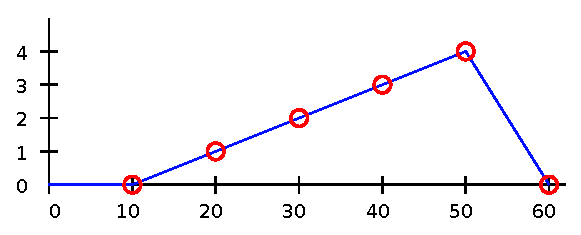
\includegraphics[width=\textwidth]{imatges/rrdtool/mostreig_regular.eps}
  \caption{Moviment d'un mòbil: perfil de velocitat en blau, punts de mostreig en vermell}
  \label{fig:rrdtool:mostreig_regular}
\end{figure}

En primer lloc, es crea una base de dades de nom \emph{velocitat.rrd} amb un temps de mostreig de 10 segons i un registre anomenat \emph{mps} que emmagatzema la velocitat del mòbil.
\begin{lstlisting}[style=sh]
export TZ=UTC
rrdtool create velocitat.rrd --start 1262304000 --step 10 \
        DS:mps:GAUGE:600:-U:U                              \ 
        RRA:AVERAGE:0.5:1:24                                                   
\end{lstlisting}


En segon lloc, s'actualitza la base de dades amb els valors $x=[0,1,2,3,4,0]$ que s'han mesurat als temps $t=[10,20,30,40,50,60]$.
\begin{lstlisting}[style=sh]
rrdtool update velocitat.rrd 1262304010:0 1262304020:1 1262304030:2 1262304040:3 1262304050:4 1262304060:0
\end{lstlisting}

Si es mostra el contingut de la base de dades, amb \verb+rrdtool dump+, es pot veure com els valors han entrat correctament:
\begin{lstlisting}
00:00:00 UTC  --> <row><v>NaN</v></row>
00:00:10 UTC  --> <row><v>0.0000000000e+00</v></row>
00:00:20 UTC  --> <row><v>1.0000000000e+00</v></row>
00:00:30 UTC  --> <row><v>2.0000000000e+00</v></row>
00:00:40 UTC  --> <row><v>3.0000000000e+00</v></row>
00:00:50 UTC  --> <row><v>4.0000000000e+00</v></row>
00:01:00 UTC  --> <row><v>0.0000000000e+00</v></row>
\end{lstlisting}


Finalment, es demana a RRDtool que faci un gràfic dels valors anteriors, el resultat es pot veure a la figura~\ref{fig:rrdtool:velocitat}:
\begin{lstlisting}[style=sh]
rrdtool graph velocitat.eps -a EPS --start 1262303999 --end 1262304060 DEF:vel=velocitat.rrd:mps:AVERAGE LINE1:vel#0000FF:"velocitat en m/s\l" -v "m/s" --x-grid SECOND:10:SECOND:10:SECOND:10:0:%X
\end{lstlisting}

\begin{figure}[htp]
  \centering
  \includegraphics[width=\textwidth]{imatges/rrdtool/velocitat.eps}
  \caption{Velocitats emmagatzemades a RRDtool d'un tipus Gauge}
  \label{fig:rrdtool:velocitat}
\end{figure}



D'aquest gràfic es desprèn com RRDtool interpreta les sèries temporals en sentit de passat. Els valors desats es representen constants en l'interval anterior al temps que els correspon. En l'exemple, a l'interval de temps (0,10] hi ha el valor 0, en l'interval (10,20] hi ha el valor 2, etc. En el temps 0, el valor és desconegut ja que no hi ha informació per l'interval anterior a zero.

Concloent, aquest és un exemple mostrejat de manera poc adequada  segons la idea de RRDtool. El mòbil de la figura~\ref{fig:rrdtool:mostreig_regular} té un perfil de velocitats mostrejat amb el valor instantani i aquest correspondria al mateix cas que mesurar una magnitud com la temperatura. Per mostrejar amb la idea de velocitat de RRDtool caldria que la velocitat fos constant; de fet, aleshores el perfil de velocitats original seria el de la figura~\ref{fig:rrdtool:velocitat}.

Si la velocitat no és constant, com és el cas de l'exemple, aleshores per complir amb la idea de RRDtool el valor mostrejat hauria d'informar de la velocitat en el darrer interval. Per exemple, amb la velocitat mitjana de cada interval ($x=[0,\ 0{,}5,\ 1{,}5,\ 2{,}5,\ 3{,}5 ,\ 2]$) ja s'aconsegueix una millor aproximació a la idea de RRDtool. Encara és més, en el concepte de RRDtool aquest exemple s'hauria de passar al domini de comptadors; és a dir mesurar l'espai recorregut en comptes de la velocitat. En els apartats següents es tractarà amb més detall els comptadors.


\subsection{Comptador monòton: \emph{Counter}}

Les dades de tipus Counter són dades provinents de comptadors. Aquestes dades no són velocitats i per tant cal aplicar transformació. 

Un comptador és un aparell de mesura que comença a zero i es va incrementant de manera contínua i monòtona en relació al paràmetre que està mesurant. A diferència d'una magnitud, un comptador no només indica el valor instantani de la variable sinó que informa dels valors des de l'última mesura. En anglès hi ha dues paraules que es tradueixen com a comptador: \emph{counter}, utilitzat en general, i \emph{meter}, utilitzat per exemple en energia elèctrica, en gas, en odometria, etc.

Per a transformar els valors d'un comptador a velocitat, a RRDtool se segueix el procediment següent.
En un moment determinat es pren el valor del comptador i al cap d'un temps definit es torna a consultar. Fent la diferència dels dos valors s'obté l'increment. Si a més es divideix per la diferència dels temps, el resultat és la mitjana del valor per unitat de temps; és a dir, una velocitat. A RRDtool el temps es mesura en segons, per tant les velocitats sempre es desen amb unitats de \emph{magnitud/s}. 
\begin{equation}\label{eq:rrdtool:rate}
c_2 \geq c_1 \longrightarrow\text{mitjana per }u.t. =\frac{c_2-c_1}{t_2-t_1}
\end{equation}
on $c_2$ i $t_2$ són el valor del comptador i el temps actual  i $c_1$ i $t_1$ són en el temps anterior.

RRDtool només emmagatzema velocitats. Per tant en les dades tipus comptador sempre calcula aquesta proporció mitjana del valor en cada període. Per exemple si el comptador mesura quilòmetres (km), el valor desat són velocitats (km/s).
Per aquesta mateixa raó, el primer valor que es desa a la base de dades no es pot calcular, ja que l'anterior no existeix, i es considera desconegut.

Els comptadors no poden decréixer però tenen un valor màxim que quan hi arriben tornen a començar des de zero. És a dir, els comptadors es poden desbordar (\emph{counter wraps}). RRDtool té en compte aquest cas i calcula l'increment real que s'ha produït. 
\begin{equation}\label{eq:rrdtool:wrap}
c_2 < c_1 \longrightarrow \text{mitjana per }u.t. =\frac{(\text{fons d'escala} -c_1)+c_2}{t_2-t_1}
\end{equation}
on ara, a diferència de l'equació~\ref{eq:rrdtool:rate}, cal tenir en compte el fons d'escala del comptador. 

Ara bé, de moment RRDtool només reconeix comptadors de 32 o 64 bits, els quals tenen rangs hexadecimals de 0 a FFFFFFFF$_h$ i de 0 a FFFFFFFFFFFFFFFF$_h$ respectivament. Si el rang del comptador és diferent d'aquests dos, el valor calculat és erroni
\footnote{En comptes del tipus \emph{counter} es pot utilitzar el tipus \emph{derive} amb el límit de velocitat mínima a zero. Llavors no es calculen valors erronis en els desbordaments sinó que es consideren desconeguts. Sigui quina sigui la manera, RRDtool no sap tractar aquests comptadors de manera adequada.\label{peu:rrdtool:counter}}.

Alguns exemples de comptador són el comptaquilòmetres d'un cotxe, els bytes transferits d'un router, la quantitat de pàgines impreses, el nombre de visitants, etc.


\paragraph{Exemple} Ara en el mòbil anterior de la figura~\ref{fig:rrdtool:velocitat}, en comptes de mesurar la velocitat es mesura l'espai recorregut com es veu a la figura~\ref{fig:rrdtool:mostreig_comptador}, també cada 10 segons. 

\begin{figure}[htp]
  \centering
  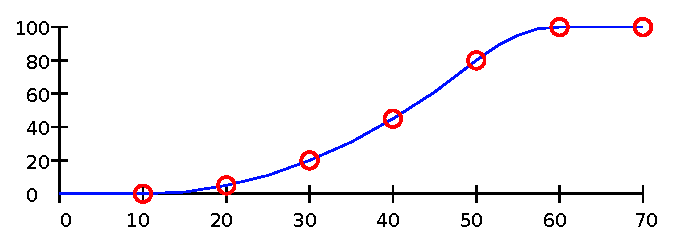
\includegraphics[width=\textwidth]{imatges/rrdtool/mostreig_comptador.eps}
  \caption{Moviment d'un mòbil: perfil d'espai recorregut en blau, punts de mesura en vermell}
  \label{fig:rrdtool:mostreig_comptador}
\end{figure}

En primer lloc, es crea una base de dades de nom \emph{comptador.rrd} amb un temps de mostreig de 10 segons i un registre anomenat \emph{mps} que emmagatzema la velocitat del mòbil però les dades d'entrada són l'espai recorregut.
\begin{lstlisting}[style=sh]
export TZ=UTC
rrdtool create comptador.rrd --start 1262304000 --step 10 \
        DS:mps:COUNTER:600:-U:U                           \ 
        RRA:AVERAGE:0.5:1:24                                                   
\end{lstlisting}

En segon lloc, s'actualitza la base de dades amb els valors $x=[0,5,20,45,80,100,100]$ que s'han mesurat als temps $t=[10,20,30,40,50,60,70]$ 

\begin{lstlisting}[style=sh]
rrdtool update comptador.rrd 1262304010:0 1262304020:5 1262304030:20 1262304040:45 1262304050:80 1262304060:100 1262304070:100
\end{lstlisting}

Si es mostra el contingut de la base de dades es pot veure com no hi ha els mateixos valors que s'han inserit; 
el gràfic de la figura~\ref{fig:rrdtool:comptador} que ha generat  RRDtool també corrobora aquestes dades:
\begin{lstlisting}
00:00:00 UTC  --> <row><v>NaN</v></row>
00:00:10 UTC  --> <row><v>NaN</v></row>
00:00:20 UTC  --> <row><v>5.0000000000e-01</v></row>
00:00:30 UTC  --> <row><v>1.5000000000e+00</v></row>
00:00:40 UTC  --> <row><v>2.5000000000e+00</v></row>
00:00:50 UTC  --> <row><v>3.5000000000e+00</v></row>
00:01:00 UTC  --> <row><v>2.0000000000e+00</v></row>
00:01:10 UTC  --> <row><v>0.0000000000e+00</v></row>
\end{lstlisting}

 
\begin{figure}[htp]
  \centering
  \includegraphics[width=\textwidth]{imatges/rrdtool/comptador.eps}
  \caption{Velocitats emmagatzemades a RRDtool d'un tipus Counter}
  \label{fig:rrdtool:comptador}
\end{figure}

En aquest gràfic, on les unitats són de metres per segon, es veu l'efecte de desar les dades en velocitat. Com que l'entrada de dades és de tipus comptador, RRDtool s'encarrega de transformar els valor a velocitat segons les equacions \ref{eq:rrdtool:rate} i \ref{eq:rrdtool:wrap} i també es compleix que el primer valor inserit s'emmagatzema com a desconegut ja que no es pot calcular. 

En referència a l'espai recorregut, es pot calcular multiplicant cada valor emmagatzemat pel temps de mostreig (10 segons). Aleshores s'obté 
$[u , 5 , 15 , 25 , 35 , 20 , 0]$
a on cada valor és l'increment d'espai recorregut en cada interval de temps corresponent; és a dir en els intervals
$[\ (0,10], (10,20], \ldots, (60,70]\ ]$.
 Per calcular l'espai recorregut total entre el temps 10 i el temps 70 s'ha de sumar aquests increments, aleshores s'obté el comptatge total de 100 metres que es correspon correctament amb el de la figura~\ref{fig:rrdtool:mostreig_comptador}.





\subsection{Comptador doble:  \emph{Derive}}

Les dades de tipus derive són de tipus comptador que tant pot incrementar com decrementar el valor; per això l'anomenem comptador doble. Aquestes dades no són velocitats i per tant cal aplicar transformació. 

La transformació a velocitat es calcula amb l'equació~\ref{eq:rrdtool:rate}, de la mateixa manera que els comptadors de tipus \emph{counter}. Però en els \emph{derive} no es té en compte el desbordament, sinó que un decrement del comptador es transforma a una velocitat negativa:  
$$
\text{mitjana per }u.t. =\frac{c_2-c_1}{t_2-t_1}
$$

Com que es desactiva el detector de desbordaments, el tipus \emph{derive} també s'utilitza per als \emph{counter} que no són ni de 32 ni de 64 bits. En aquests casos es configura el límit mínim de velocitat a zero i quan hi ha el desbordament\footnote{Això no es pot considerar una bona solució, vegeu nota~\ref{peu:rrdtool:counter}.} el valor transformat es considera desconegut, ja que la velocitat calculada és inferior al límit imposat de valor zero. 

Alguns exemples de comptador \emph{derive} són una bomba de cabal que pot bombejar o succionar, un comptador elèctric que mesura el total d'energia consumida menys la produïda, el balanç de població que emigra menys la que immigra, el saldo d'una llibreta que té ingressos i despeses, la quantitat de productes d'una màquina de \emph{vending}, etc. 


\paragraph{Exemple} Es mesura el saldo d'una llibreta d'estalvi que inicialment està a 0\euro, al cap de 10 segons rep un ingrés de 10\euro, al cap de 10 segons rep 20\euro\ i al cap de 10 segons té una despesa de 15\euro. 

Els valors que va prenent la llibreta (el comptador) es poden veure a la figura~\ref{fig:rrdtool:mostreig_derive}. Les mostres es prenen a l'instant abans que es faci l'operació d'ingrés o despesa; és a dir que la llibreta mostra el valor que ha tingut a l'interval anterior, la qual és la manera com s'entenen les sèries temporals a RRDtool. 

\begin{figure}[htp]
  \centering
  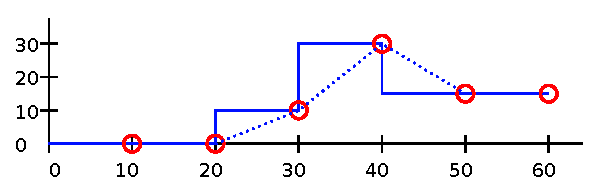
\includegraphics[width=\textwidth]{imatges/rrdtool/mostreig_derive.eps}
  \caption{Llibreta d'estalvi: valor del saldo en blau, punts de mesura en vermell}
  \label{fig:rrdtool:mostreig_derive}
\end{figure}

A més, RRDtool entén que les variables mesurades són contínues. Per tant amb les mesures fetes de la llibreta entén que el valor s'ha incrementat de manera contínua en tot l'interval. Això es pot observar a la línia discontínua de la figura~\ref{fig:rrdtool:mostreig_derive}, que és l'aproximació que fa RRDtool ja que només es guarda la velocitat mitjana a l'interval.

Es crea una base de dades de nom \emph{derive.rrd} amb un temps de mostreig de 10 segons i un registre anomenat \emph{eurps} que emmagatzema la velocitat del comptador (del saldo de la llibreta) a partir de les lectures del saldo. 

\begin{lstlisting}[style=sh]
export TZ=UTC
rrdtool create derive.rrd --start 1262304000 --step 10 \
        DS:eurps:DERIVE:600:-U:U                       \ 
        RRA:AVERAGE:0.5:1:24                                                   
\end{lstlisting}


S'actualitza la base de dades amb els valors $x=[0,0,10,30,15,15]$ que s'han mesurat als temps $t=[10,20,30,40,50,60]$ 

\begin{lstlisting}[style=sh]
rrdtool update derive.rrd 1262304010:0 1262304020:0 1262304030:10 1262304040:30 1262304050:15 1262304060:15
\end{lstlisting}

A continuació es mostren els valors emmagatzemats i a la figura~\ref{fig:rrdtool:derive} es mostra el gràfic que genera RRDtool:
\begin{lstlisting}
00:00:00 UTC  --> <row><v>NaN</v></row>
00:00:10 UTC  --> <row><v>NaN</v></row>
00:00:20 UTC  --> <row><v>0.0000000000e+00</v></row>
00:00:30 UTC  --> <row><v>1.0000000000e+00</v></row>
00:00:40 UTC  --> <row><v>2.0000000000e+00</v></row>
00:00:50 UTC  --> <row><v>-1.5000000000e+00</v></row>
00:01:00 UTC  --> <row><v>0.0000000000e+00</v></row>
\end{lstlisting}


\begin{figure}[htp]
  \centering
  \includegraphics[width=\textwidth]{imatges/rrdtool/derive.eps}
  \caption{Velocitats emmagatzemades a RRDtool d'un tipus Derive}
  \label{fig:rrdtool:derive}
\end{figure}

Aquest gràfic és com l'analitzat en l'exemple dels tipus \emph{counter} (figura~\ref{fig:rrdtool:comptador}), amb la diferència que ara en els \emph{derive} hi apareixen velocitats negatives. 
Com s'ha fet en els \emph{counter}, es pot calcular els increments de saldo de cada interval multiplicant les velocitats pel temps de mostreig. Aleshores els increments de saldo són $[u,0,10,20,-15,0]$ que sumats donen correctament els 15\euro\ de saldo final de la figura~\ref{fig:rrdtool:mostreig_derive}.


\subsection{Comptador relatiu: \emph{Absolute}}

Les dades de tipus Absolute són de tipus comptador d'increments; per això l'anomenen comptador relatiu. Aquestes dades no són velocitats i per tant cal aplicar transformació. 

Un comptador d'increments mesura directament la diferència des de l'última lectura, es pot veure com un comptador que es posa a zero a cada lectura. Per tant, per transformar les mesures a velocitat es divideix l'increment per la diferència de temps
$$
\text{mitjana per }u.t. =\frac{\Delta c}{t_2-t_1}
$$
on ara, a diferència de l'equació~\ref{eq:rrdtool:rate}, es mesura directament el comptatge ($\Delta c$) des de la mesura anterior.

Els increments mesurats poden ser positius o negatius; és a dir com en el cas \emph{derive} les velocitats resultants poden ser positives o negatives. Per tant, el tipus \emph{absolute} és el mateix que el \emph{derive} amb la diferència que el valor mesurat, el qual és el valor actual del comptador,  és un increment.

El primer valor que es desa a la base de dades ara es pot calcular, a diferència dels comptadors \emph{counter} i \emph{derive}. En aquest dos cal calcular l'increment de comptatge i en el primer valor és desconegut, ja que podria ser erroni suposar-lo com a zero. En el cas del comptador \emph{absolute} també cal indicar quin és el temps inicial, però aquest es considera que és el mateix que el d'inici de la base de dades.

Alguns exemples de comptador \emph{absolute} són els mateixos que en el \emph{derive} però mesurats de manera relativa: increments de bombeig o succió d'una bomba, la mesura de l'energia elèctrica en un cert temps, els increments de població degut a la migració, els registres a una llibreta, la venda o repostatge de productes, etc.

\paragraph{Exemple} Com en l'exemple del tipus \emph{derive} (figura~\ref{fig:rrdtool:mostreig_derive}), es mesura el saldo d'una llibreta d'estalvi. Ara, però, les mesures de comptador són les operacions d'ingrés o de despesa. El saldo pren els mateixos valors que en l'exemple anterior però ara les mesures són els increments, positius o negatius, que es poden veure a la figura~\ref{fig:rrdtool:mostreig_absolute}. 

\begin{figure}[htp]
  \centering
  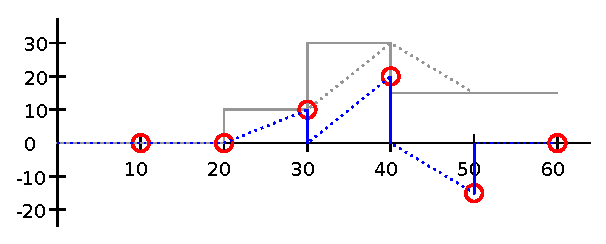
\includegraphics[width=\textwidth]{imatges/rrdtool/mostreig_absolute.eps}
  \caption{Llibreta d'estalvi: increments de saldo en blau, punts de mesura en vermell, saldo en gris}
  \label{fig:rrdtool:mostreig_absolute}
\end{figure}

Les línies discontínues segueixen mostrant, com a la figura~\ref{fig:rrdtool:mostreig_derive}, l'aproximació que RRDtool fa del comptador com a variable contínua. 


Es crea una base de dades de nom \emph{absolute.rrd} amb un temps de mostreig de 10 segons i un registre anomenat \emph{eurps} que emmagatzema la velocitat del comptador (el saldo de la llibreta) a partir dels increments de saldo. 
\begin{lstlisting}[style=sh]
export TZ=UTC
rrdtool create absolute.rrd --start 1262304000 --step 10 \
        DS:eurps:ABSOLUTE:600:-U:U                        \ 
        RRA:AVERAGE:0.5:1:24                                                   
\end{lstlisting}


S'actualitza la base de dades amb els valors $x=[0,0,10,20,-15,0]$ que s'han mesurat als temps $t=[10,20,30,40,50,60]$ 
\begin{lstlisting}[style=sh]
rrdtool update absolute.rrd 1262304010:0 1262304020:0 1262304030:10 1262304040:20 1262304050:-15 1262304060:0
\end{lstlisting}

A continuació es mostren els valors emmagatzemats i a la figura~\ref{fig:rrdtool:absolute} es mostra el gràfic que genera RRDtool; és idèntic a la figura~\ref{fig:rrdtool:derive} però ara el primer valor és conegut.:
\begin{lstlisting}
00:00:00 UTC  --> <row><v>NaN</v></row>
00:00:10 UTC  --> <row><v>0.0000000000e+00</v></row>
00:00:20 UTC  --> <row><v>0.0000000000e+00</v></row>
00:00:30 UTC  --> <row><v>1.0000000000e+00</v></row>
00:00:40 UTC  --> <row><v>2.0000000000e+00</v></row>
00:00:50 UTC  --> <row><v>-1.5000000000e+00</v></row>
00:01:00 UTC  --> <row><v>0.0000000000e+00</v></row>
\end{lstlisting}


\begin{figure}[htp]
  \centering
  \includegraphics[width=\textwidth]{imatges/rrdtool/absolute.eps}
  \caption{Velocitats emmagatzemades a RRDtool d'un tipus Absolute}
  \label{fig:rrdtool:absolute}
\end{figure}

D'aquest gràfic, com en el casos \emph{derive} i \emph{counter}, es pot obtenir els increments de comptatge a cada interval si es multiplica cada valor pel temps de mostreig (10 segons). Aquests valors es podrien observar en un gràfic de barres, tot i que RRDtool només treballa amb variables velocitat contínues i per tant no pot mostrar exactament aquest gràfics de barres del comptador. A la figura~\ref{fig:rrdtool:comptador_barres} s'utilitza RRDtool perquè dibuixi els valors pintant l'àrea i multiplicant l'escala de l'eix Y per 10; perquè fos un gràfic de barres cal imaginar que a l'eix X hi ha les etiquetes corresponents als intervals: $(0,10], (10,20], \ldots, (50,60]$ i que cada un d'aquest intervals és una barra.

\begin{figure}[htp]
  \centering
  \includegraphics[width=\textwidth]{imatges/rrdtool/comptador_barres.eps}
  \caption{Gràfic de barres a RRDtool d'un comptador}
  \label{fig:rrdtool:comptador_barres}
\end{figure}

Ara bé, RRDtool sí que té funcions per tractar amb càlculs típics dels comptadors, per exemple calcular el total del comptador en un interval de temps donat. En aquest cas, el total del comptador des de l'inici fins a una data correspon al saldo de la llibreta en aquella data. A continuació es calcula el saldo des del temps 0 fins al temps 60, el qual correspon als 15\euro\ de la figura~\ref{fig:rrdtool:mostreig_absolute}.:
\begin{lstlisting}[style=sh]
rrdtool graphv absolute.eps -a EPS --start 1262303999 --end 1262304060 DEF:saldo=absolute.rrd:eurps:AVERAGE VDEF:tot=saldo,TOTAL PRINT:tot:%lf\EUR/s
\end{lstlisting}

\begin{lstlisting}
print[0] = "15.000000EUR/s"
\end{lstlisting}

\section[Normalització]{Normalització de l'interval}
\label{sec:rrdtool-etapes:normalitzacio}

RRDtool emmagatzema les dades a intervals regulars, és a dir en el temps de mostreig desitjat (anomenat \emph{step}). Com que a la pràctica és difícil complir-lo amb exactitud, cal modificar les dades perquè encaixin en aquest temps; és a dir s'ha de normalitzar l'interval de la sèrie temporal.

Per a modificar els valors de la sèrie temporal, en el context de velocitat vist a l'apartat anterior es pot plantejar una modificació de dades que tracti de mantenir l'àrea de sota la corba. La interpretació física és que es manté la quantitat total de magnitud.
Per exemple si les dades són velocitats lineals en m/s es pot entendre el problema com que es modifica la velocitat però es manté l'espai recorregut. O bé si les dades són comptadors, com que s'ha desat la velocitat s'entén que s'està mantenint la quantitat total.

Així doncs, el problema a resoldre és el següent. Donada una sèrie temporal acotada a un temps final $T_F$
$$%
S=\{\mathbf{X(t)}; t=t_0,t_1,t_2,\ldots,t_F\}
$$
que no té un període de mesura regular 
$$
t_{i+1}\neq t_{i} + T 
$$
es vol convertir a una sèrie temporal normalitzada amb interval regulars tal que ara $T$ correspongui al període de mostreig $t_m$:
$$%
S^N=\{\mathbf{X^N(t^N)}; t^N=t_0,t_1,t_2,\ldots,t_k\}
$$
$$
t^N_{k+1}= t^N_{k} + t_m 
$$
$$
t^N_k < T_F
$$
on $N$ indica que els valors i els temps ara contenen els valors normalitzats:
$$
\mathbf{X^N}= [x^N(t^N_0),x^N(t^N_1),\ldots,x^N(t^N_{T_i})]
$$

En resum, el vector de mesures té la forma 
$$
\mathbf{X(t)} = [x_0,x_1,\ldots,x_{F-1},x_F]
$$
i amb la mateixa mida el vector de temps de mesures
$$
\mathbf{t}=[t_0,t_1 \ldots, t_{T_f-1}, t_{T_f} ]
$$

Però el vector de valors normalitzats té una mida diferent 
$$
\mathbf{X^N(t^N)} = [x^N_0, x^N_1, \ldots,x^N_k ]
$$
on el vector de temps de mostreig normalitzats té la forma
$$
\mathbf{t^N}=[0,t_m, 2t_m,3t_m, \ldots kt_m ]
$$


A l'hora de convertir la sèrie temporal RRDtool utilitza el criteri de mantenir constant l'àrea sota la corba; a l'apartat~\ref{sec:rrdtool-etapes:gauge} s'ha vist com RRDtool representa les sèries temporals en velocitat i en passat. En els exemples d'aquest apartat, però, les mesures es feien en el temps de mostreig exacte, a continuació es mostrarà com RRDtool gestiona els casos en els que les mostres no coincideixen amb el temps de mostreig.

\subsection{Mostreig en temps real}

En un primer cas, la sèrie temporal original està mostrejada amb un únic valor a cada interval, tal com es faria en un sistema en temps real 
$$
\mathbf{X(t)}= [x(t_0)\ldots,x(t_{T_f-1}),x(t_{T_f})]
$$
$$
0< t_0 < t^N_1 < \cdots <   t^N_{i-1}<t_{T_f-1} < t^N_i < t_{T_f}
$$ 

En aquest cas, la sèrie temporal no té intervals regulars però sí que hi ha garantits uns terminis temporals en els que es disposa d'un valor i només hi ha un valor a cada interval:
$$
t_{i+1}\neq t_{i} + T 
$$
$$
t_{i+1} - t_{i} \leq t_m 
$$

A continuació es detalla com RRDtool normalitza la sèrie temporal en l'interval $[t^N_{i-1},t^N_i]$, es pot veure una interpretació gràfica a la figura~\ref{fig:rrdtool:normalitzacio}.

\begin{figure}[htp]
  \centering
  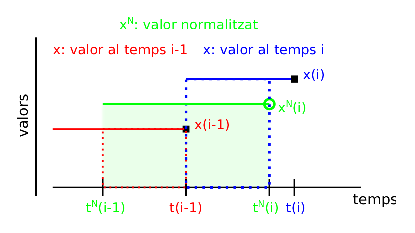
\includegraphics[width=\textwidth]{imatges/rrdtool/normalitzacio.eps}
  \caption{Normalització d'un interval}
  \label{fig:rrdtool:normalitzacio}
\end{figure}


Per una banda, es calcula l'àrea en l'interval seleccionat a partir dels valors mesurats
\[
A([t^N_{i-1},t^N_i]) = A([t^N_{i-1},t_{i-1}])+A([t_{i-1},t^N_i]) = ( t_{i-1} - t^N_{i-1})x_{i-1} + ( t^N_{i} - t_{i-1} )x_{i}
\]
i per altra banda, la normalització de l'interval s'expressa amb un valor de velocitat $X^N_i$ que es representa en el temps  $t^N_i$ degut a que RRDtool interpreta els valors en passat (constants en l'interval anterior)
\[
A^N = (  t^N_i - t^N_{i-1} )x^N_i  = t_m x^N_i
\]
Aleshores, s'igualen les dues expressions per tal que en normalitzar es conservi l'àrea en l'interval
\[
A^N=A([t^N_{i-1},t^N_i])
\]
d'on aïllant s'obté l'equació del valor normalitzat 
\begin{equation}\label{eq:rrdtool-etapes:normalitza}
x^N_i= \frac{(t_{i-1}-t^N_{i-1})x_{i-1} + (t^N_i-t_{i-1})x_i  }{t_m}
\end{equation}


El mateix es pot aplicar per tots els intervals de $\mathbf{X}$ per obtenir $\mathbf{X^N}$.



\paragraph{Exemple}


Agafem una nova base de dades velocitat.rrd i ara l'actualitzem amb el mateix perfil de velocitat de la figura~\ref{fig:rrdtool:mostreig_regular} però mostrejat de manera irregular com es veu a la figura~\ref{fig:rrdtool:mostreig_irregular}. A cada interval de mostreig hi segueix havent una mesura, i per tant compleixen el període de mostreig, però el temps de mostreig és irregular. Així ara els valors de velocitat mesurats són $x=[0, 0{,}5 , 1 , 2{,}8 , 3{,}2 , 2 , 0]$ en els temps $t=[10,15,20,38,42,55,65]$.


\begin{figure}[htp]
  \centering
  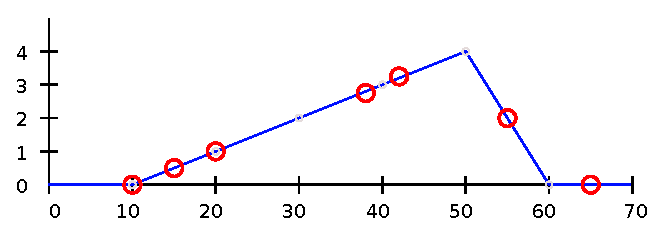
\includegraphics[width=\textwidth]{imatges/rrdtool/mostreig_irregular.eps}
  \caption{Mostreig en temps real: perfil de velocitat en blau, punts de mesura irregulars en vermell, període de mostreig de 10 segons}
  \label{fig:rrdtool:mostreig_irregular}
\end{figure}

S'insereixen els valors a la base de dades:
\begin{lstlisting}[style=sh]
rrdtool update velocitat.rrd 1262304010:0 1262304015:0.5 1262304020:1 1262304038:2.8 1262304042:3.2 1262304055:2 1262304065:0
\end{lstlisting}

A continuació es mostren els valors emmagatzemats i el gràfic que genera RRDtool (figura~\ref{fig:rrdtool:velocitat_irregular}):
\begin{lstlisting}
00:00:00 UTC  --> <row><v>NaN</v></row>
00:00:10 UTC  --> <row><v>0.0000000000e+00</v></row>
00:00:20 UTC  --> <row><v>7.5000000000e-01</v></row>
00:00:30 UTC  --> <row><v>2.8000000000e+00</v></row>
00:00:40 UTC  --> <row><v>2.8800000000e+00</v></row>
00:00:50 UTC  --> <row><v>2.2400000000e+00</v></row>
00:01:00 UTC  --> <row><v>1.0000000000e+00</v></row>
\end{lstlisting}


\begin{figure}[htp]
  \centering
  \includegraphics[width=\textwidth]{imatges/rrdtool/velocitat_irregular.eps}
  \caption{Valors emmagatzemats a RRDtool d'un mostreig en temps real}
  \label{fig:rrdtool:velocitat_irregular}
\end{figure}

Aplicant l'equació~\ref{eq:rrdtool-etapes:normalitza} als valors mesurats es pot comprovar que s'obtenen els valors normalitzats calculats per RRDtool 
$\mathbf{X^N}=[u , 0 , 0{,}75 , 2{,}8 , 2{,}88 , 2{,}24 , 1]$. 
Cal notar que a RRDtool el primer valor normalitzat, el qual correspon al temps $t^N_0$, és desconegut ja que no s'admeten insercions en el temps $t_0$.


\subsection{Ultramostreig}

En la normalització anterior de mostreig en temps real, en cada període de mostreig només hi havia una mesura. Ara bé, RRDtool permet que en cada interval hi hagi més d'una mesura i per tant hi pot haver més d'un valor a l'hora de normalitzar; anomenem aquest mostreig com ultramostreig (\emph{upsampling}), representat a la figura~\ref{fig:rrdtool-etapes:ultramostreig}.
$$
\mathbf{X(t)}= [x(t_0)\ldots,x(t_{T_f-k}),\cdots,x(t_{T_f-2}),x(t_{T_f-1}),x(t_{T_f})]
$$
$$
0< t_0 < t^N_1 < \cdots <   t^N_{i-1}<t_{T_f-k} <\cdots< t_{T_f-1} < t^N_i < t_{T_f}
$$

\begin{figure}[tbp]
  \centering
  \begin{tikzpicture}
    \begin{axis}[
        xlabel=temps ,
        ylabel= valor,
        xticklabels={0,$t_1^N$,$\ldots$,$t_{i-1}^N$,$t_i^N$},
        ]
    \addplot[ycomb,blue] coordinates {
        (0,10)
        (10,10)
        (20,10)
        (30,10)
        (40,10)
    }; 
 
    \addplot[only marks,mark=*,red] coordinates {
        (5,1)
        (32,2)
        (35,3)
        (38,4)
        (45,5)
    };

    \node[above] at (axis cs:5,1) {$t_0$};
    \node[below] at (axis cs:32,2) {$t_{T_f -k}$};
    \node[below] at (axis cs:35,3) {$\ldots$};
    \node[above] at (axis cs:38,4) {$t_{T_f -1}$};
    \node[above] at (axis cs:45,5) {$t_{T_f}$};

    \end{axis}
  \end{tikzpicture}
  \caption{Representació d'ultramostreig}
  \label{fig:rrdtool-etapes:ultramostreig}
\end{figure}

Aleshores, el valor normalitzat es calcula de la mateixa manera que a l'equació~\ref{eq:rrdtool-etapes:normalitza}, però ara el càlcul és una ponderació pel temps de tots els valors que cauen a dins de l'interval de normalització
\begin{equation}\label{eq:rrdtool:ultramostreig}
x^N_i = \frac{ (t_{T_f-k}-t^N_{i-1})x_{f-k} + \cdots + (t_{T_f-1}-t_{T_f-2})x_{f-1} + (t^N_i-t_{T_f-1})x_f }{t_m}
\end{equation}


Seguint aquesta equació de manera iterativa, es pot calcular el vector de valors normalitzats $\mathbf{X^N}$  per tots els $\mathbf{X(t)}$ amb l'algoritme següent:

\begin{lstlisting}[mathescape=true]  
Normalització d'una sèrie temporal amb ultramostreig 
a períodes de mostreig regulars 
INPUT: 
      vector de valors $\mathbf{X} = [x_0,x_1,\ldots,x_f]$ 
      vector de temps $\mathbf{t} = [t_0,t_1,\ldots,t_f]$
      període de mostreig regular  $t_m$
OUTPUT: 
      vector de valors normalitzats $\mathbf{X^N} = [x_0^N,x_1^N,\ldots,x_k^N]$

$x^N_0$ := unknown
$t^N_0$ := 0
$t^N_1$ := $t_0^N$ + $t_m$
i := 1

$A$ := $x_0t_0$   <-- àrea acumulada inicial 
k := 1

mentre k $\leq$ dim(x) fes

    si $t_k < t_i^N$ llavors
        $A$ := $A + x_k( t_k-t_{k-1}) $ <-- acumulació
        k := k+1
    sino 
        $x_i^N$ := $\dfrac{A + x_k( t_i^N-t_{k-1} )}{t_m}$

        $t_{i+1}^N$ := $t_i^N$ + $t_m$
        $A$ := $x_k*( t_k-t_i^N )$ <-- àrea acumulada inicial 
        k := k+1
        i := i+1
    fsi 

fmentre

\end{lstlisting}

\paragraph{Exemple}

Agafem una nova base de dades velocitat.rrd i ara l'actualitzem amb el mateix perfil de velocitat de la figura~\ref{fig:rrdtool:mostreig_regular} però amb més mostres en algun interval com es veu a la figura~\ref{fig:rrdtool:ultramostreig}. A cada interval de mostreig hi segueix havent com a mínim una mesura i compleixen el període de mostreig però en algun interval hi ha més d'una mostra. Així ara el valors de velocitat mesurats són $x=[0 , 0{,}5 , 0{,}8 , 1 , 2{,}8 , 3{,}2 , 3{,}5 , 3{,}8 , 2 , 0]$ en els temps $t=[10 , 15 , 18, 20, 38, 42, 45, 48, 55, 65]$.


\begin{figure}[htp]
  \centering
  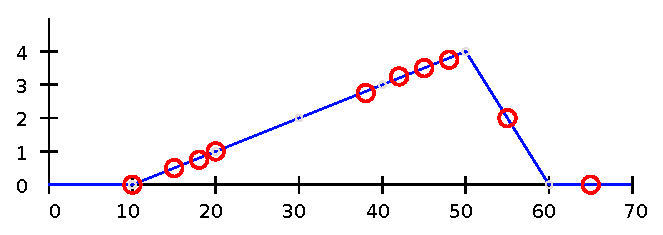
\includegraphics[width=\textwidth]{imatges/rrdtool/sobremostreig.eps}
  \caption{Ultramostreig: perfil de velocitat en blau, punts de mesura (alguns ultramostrejats) en vermell, període de mostreig de 10 segons}
  \label{fig:rrdtool:ultramostreig}
\end{figure}

S'insereixen els valors a la base de dades:
\begin{lstlisting}[style=sh]
rrdtool update velocitat.rrd 1262304010:0 1262304015:0.5 1262304018:0.8 1262304020:1 1262304038:2.8 1262304042:3.2 1262304045:3.5 1262304048:3.8 1262304055:2 1262304065:0
\end{lstlisting}

A continuació es mostren els valors emmagatzemats i el gràfic que genera RRDtool (figura~\ref{fig:rrdtool:velocitat_ultramostrejada}):

\begin{lstlisting}
00:00:00 UTC  --> <row><v>NaN</v></row>
00:00:10 UTC  --> <row><v>0.0000000000e+00</v></row>
00:00:20 UTC  --> <row><v>6.9000000000e-01</v></row>
00:00:30 UTC  --> <row><v>2.8000000000e+00</v></row>
00:00:40 UTC  --> <row><v>2.8800000000e+00</v></row>
00:00:50 UTC  --> <row><v>3.2300000000e+00</v></row>
00:01:00 UTC  --> <row><v>1.0000000000e+00</v></row>
\end{lstlisting}


\begin{figure}[htp]
  \centering
  \includegraphics[width=\textwidth]{imatges/rrdtool/velocitat_sobremostrejada.eps}
  \caption{Valors emmagatzemats a RRDtool d'un ultramostreig}
  \label{fig:rrdtool:velocitat_ultramostrejada}
\end{figure}

Respecte a la figura~\ref{fig:rrdtool:velocitat_irregular} del cas de mostreig en temps real, ara només han canviat els valors dels intervals ultramostrejats mentre que els altres intervals continuen valent el mateix: $\mathbf{X^N}=[u , 0 , \underline{0{,}69} , 2{,}8 , 2{,}88 , \underline{2{,}24} , 1]$. Els valors que canvien són molt semblants als anteriors, però es pot dir que es té una millor aproximació a la velocitat real ja que en aquests intervals s'ha mostrejat més.

\subsection{Inframostreig}

Per altra banda, quan en un interval no hi ha cap mesura, és a dir que el temps de mostreig supera al període de mostreig, s'anomenem inframostreig (\emph{downsampling}).
$$
\mathbf{X(t)}= [x(t_0)\ldots,x(t_{T_f-1}),x(t_{T_f})]
$$
$$
t^N_{i-m-1} < t_{T_f-1} < t^N_{i-m} < \cdots < t^N_{i-1} < t^N_i < t_{T_f}
$$ 

\begin{figure}[tbp]
  \centering
  \begin{tikzpicture}
    \begin{axis}[
        width=10cm,scale only axis, height=5cm,
        xlabel=temps ,
        ylabel= valor,
        xticklabels={0,$t_1^N$,$\ldots$,$t_{i-m-1}^N$,$t_{i-m}^N$,$\ldots$,$t_{i-1}^N$,$t_i^N$},
        ]
    \addplot[ycomb,blue] coordinates {
        (0,10)
        (10,10)
        (20,10)
        (30,10)
        (40,10)
        (50,10)
        (60,10)
        (70,10)
    }; 
 
    \addplot[only marks,mark=*,red] coordinates {
        (5,1)
        (32,2)
        (35,3)
        (38,4)
        (75,5)
    };

    \node[above] at (axis cs:5,1) {$t_0$};
    \node[below] at (axis cs:32,2) {$t_{T_f -k}$};
    \node[below] at (axis cs:35,3) {$\ldots$};
    \node[above] at (axis cs:38,4) {$t_{T_f -1}$};
    \node[above] at (axis cs:75,5) {$t_{T_f}$};

    \end{axis}
  \end{tikzpicture}
  \caption{Representació d'inframostreig}
  \label{fig:rrdtool-etapes:inframostreig}
\end{figure}


Llavors per normalitzar amb inframostreig RRDtool utilitza el valor del següent interval. En aquest cas se suposa que les mesures no tenen termini, més endavant s'afegeix el problema del termini (vegeu apartat~\ref{sec:rrdtool-etapes:termini}).

És a dir, quan entre dues mesures hi ha més temps que el temps de mostreig llavors el valor de l'última mesura $\mathbf{x}(t_{T_f})$ s'expandeix enrere fins arribar a l'altra $\mathbf{x}(t_{T_f-1})$  i es calcula el valor normalitzat d'aquest gran interval. Si hi ha inframostreig però no hi ha ultramostreig
$$
t^N_{i-m-1} < t_{T_f-1} < t^N_{i-m} 
$$ 
el valor normalitzat és:
$$
x^N = \frac{ (t_{T_f-1}-t^N_{i-m-1})x_{f-1} + (t^N_i-t_{T_f-1})x_f }{t^N_i - t^N_{i-m-1}}
$$

Generalitzant, si alhora hi ha inframostreig i ultramostreig, representat a la figura~\ref{fig:rrdtool-etapes:inframostreig},
\[
t^N_{i-m-1} <  t_{T_f-k} <\cdots< t_{T_f-1}  < t^N_{i-m} 
\] 
el valor normalitzat es calcula de la mateixa manera que a l'equació~\ref{eq:rrdtool:ultramostreig}, però en l'interval $[t^N_{i-m-1},t^N_i]$:
\begin{equation}\label{eq:rrdtool:inframostreig}
x^N = \frac{ (t_{T_f-k}-t^N_{i-m-1})x_{f-k} + \cdots + (t_{T_f-1}-t_{T_f-2})x_{f-1} + (t^N_{i}-t_{T_f-1})x_f }{t^N_i - t^N_{i-m-1}}
\end{equation}

Finalment, aquest valor normalitzat per inframostreig, hi hagi ultramostreig o no, és utilitzat en tots els intervals afectats:
\[
x^N = x^N_{i-m} = \cdots = x^N_{i}
\]


Es modifica l'algoritme de càlcul iteratiu anterior segons aquest inframostreig:

\begin{lstlisting}[mathescape=true]
Normalització d'una sèrie temporal amb inframostreig
a períodes de mostreig regulars 
INPUT: 
      vector de valors $\mathbf{X} = [x_0,x_1,\ldots,x_f]$ 
      vector de temps $\mathbf{t} = [t_0,t_1,\ldots,t_f]$
      període de mostreig regular  $t_m$
OUTPUT: 
      vector de valors normalitzats $\mathbf{X^N} = [x_0^N,x_1^N,\ldots,x_k^N]$

$x_0^N$ := unknown
$t_0^N$ := 0
$t_1^N$ := $t_0^N$ + $t_m$
i := 1

$A$ := $x_0t_0$
k := 1

mentre k $\leq$ dim(x) fes
    si $t_k < t_i^N$ llavors
        $A$ := $A + x_k( t_k-t_{k-1} )$
        k := k+1
    sino 
        $N_{inf}$ := $(t_k-t_i^N)$ div $t_m$ <-- n. d'intervals amb inframostreig

        $x_i^N$ := $\dfrac{A + x_k( t_i^N-t_{k-1} ) + x_k \cdot N_{inf} \cdot t_m}{t_m  (1+N_{inf})}$

        mateix valor per cada interval amb inframostreig
        $x_{i+N_{inf}}^N$ := $\,\cdots\,$ := $x_{i+1}^N$ := $x_i^N$
        $t_{i+1}^N$ := $t_i^N + (N_{inf}+1) t_m$
        i := i + ($N_{inf}$+1)
                
        $A$ := $x_k( t_k-t_{i-1}^N )$
        k := k+1
    fsi 
fmentre
\end{lstlisting}

\paragraph{Exemple}

Agafem una nova base de dades velocitat.rrd i ara l'actualitzem amb el mateix perfil de velocitat de la figura~\ref{fig:rrdtool:mostreig_regular} però en algun interval no hi ha mostres, com es veu a la figura~\ref{fig:rrdtool:inframostreig}. És important ressaltar que aquests intervals no compleixen el període de mostreig
 Així ara el valors de velocitat mesurats són $x=[0, 0{,}5 , 2{,}5 , 3{,}8 , 2 , 0]$ en els temps $t=[10, 15, 35, 48, 55, 65]$.

\begin{figure}[htp]
  \centering
  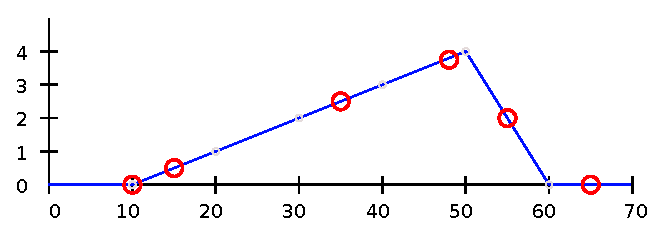
\includegraphics[width=\textwidth]{imatges/rrdtool/inframostreig.eps}
  \caption{Inframostreig: perfil de velocitat en blau, punts de mesura (alguns inframostrejats) en vermell, període de mostreig de 10 segons}
  \label{fig:rrdtool:inframostreig}
\end{figure}



S'insereixen els valors a la base de dades:
\begin{lstlisting}[style=sh]
rrdtool update velocitat.rrd 1262304010:0 1262304015:0.5 1262304035:2.5 1262304048:3.8 1262304055:2 1262304065:0
\end{lstlisting}

A continuació es mostren els valors emmagatzemats i el gràfic que genera RRDtool (figura~\ref{fig:rrdtool:velocitat_inframostrejada}):
\begin{lstlisting}
00:00:00 UTC  --> <row><v>NaN</v></row>
00:00:10 UTC  --> <row><v>0.0000000000e+00</v></row>
00:00:20 UTC  --> <row><v>2.0000000000e+00</v></row>
00:00:30 UTC  --> <row><v>2.0000000000e+00</v></row>
00:00:40 UTC  --> <row><v>3.1500000000e+00</v></row>
00:00:50 UTC  --> <row><v>3.4400000000e+00</v></row>
00:01:00 UTC  --> <row><v>1.0000000000e+00</v></row>
\end{lstlisting}


\begin{figure}[htp]
  \centering
  \includegraphics[width=\textwidth]{imatges/rrdtool/velocitat_inframostrejada.eps}
  \caption{Valors emmagatzemats a RRDtool d'un inframostreig}
  \label{fig:rrdtool:velocitat_inframostrejada}
\end{figure}


Respecte a la figura~\ref{fig:rrdtool:velocitat_irregular} del cas de mostreig en temps real, aquest gràfic només es diferencia en els intervals inframostrejats.
Ara els intervals afectats per l'inframostreig $(10,20]$ i $(20,30]$ tenen el mateix valor de 2, el qual resulta d'aplicar l'equació~\ref{eq:rrdtool:inframostreig}:  
$
x_{20}^N = x_{30}^N  = 
\frac{ (15-10) 0{,}5 + (30-15) 2{,}5 }{30 - 10}
= 2
$.
En aquests dos intervals hi ha una pitjor aproximació a la velocitat real ja que s'ha mostrejat molt poc.



\subsection{Tractament de dades desconegudes}

En les seccions anteriors, les mesures de les sèries temporals sempre tenen un valor numèric. En concret són números reals ($\mathbb{R}$), els quals es representen informàticament amb el format numèric de precisió doble seguint l'estàndard IEEE 754,~\cite{wiki:ieee754}.
 
Però les mesures, a més a més de tenir un valor, també poden ser desconegudes (\emph{unknown data}); és a dir, que no existeixin o que s'ignorin (es descartin).  Aquests valors desconeguts també estan contemplats a l'estàndard IEEE 754 i es representen  amb el valor numèric especial NaN (\emph{Not a Number}). 

L'algoritme de normalització d'intervals ha de saber manipular les mostres amb mesures desconegudes. En el cas de RRDtool, les dades desconegudes poden venir per tres vies:

\begin{itemize}
\item la mesura no existeix,
\item el temps de mesura ha superat el termini o
\item el valor de mesura està fora dels límits.
\end{itemize}

A continuació es detallen aquestes tres vies i al final es modifica l'algoritme de normalització en concordança amb el tractament d'aquestes dades desconegudes.

\subsubsection{Mesura inexistent}

Una mesura no existeix quan no s'ha pogut establir contacte amb el sensor o quan aquest retorna valors que no són númerics. Quan una mesura no existeix, es considera desconeguda i s'insereix a la base de dades amb el valor 'U' (\emph{unknown}) tot i que queda representat amb el valor NaN segons l'estàndard IEEE 754. 


Les mesures també es desconeixen quan s'inicialitza la base de dades. A l'inici d'una base de dades RRDtool es creen tots els registres fins al temps actual però aquestes mesures no han existit mai; per tant prenen 'desconegut' com a valor.


\paragraph{Exemple} S'insereix una dada amb valor conegut i l'altra amb valor desconegut

\begin{lstlisting}[style=sh]
rrdtool update velocitat.rrd 1262304010:1 1262304020:U 
\end{lstlisting}

\begin{lstlisting}
23:59:30 UTC  --> <row><v>NaN</v></row>
23:59:40 UTC  --> <row><v>NaN</v></row>
23:59:50 UTC  --> <row><v>NaN</v></row>
00:00:00 UTC  --> <row><v>NaN</v></row>
00:00:10 UTC  --> <row><v>1.0000000000e+00</v></row>
00:00:20 UTC  --> <row><v>NaN</v></row>
\end{lstlisting}

Per una banda, tots els valors anteriors al temps 0 (aquest inclòs) són desconeguts perquè no es coneix res abans que s'inicialitzi la base de dades. Per altra banda, s'ha inserit un valor numèric en el temps 10 i el valor 'desconegut' en el temps 20.



\subsubsection{Temps de termini}
\label{sec:rrdtool-etapes:termini}

El temps de termini, el qual RRDtool anomena \emph{heartbeat} ($t_h$), és el temps màxim que s'admet entre dues mesures. La mesura actual s'ignora si ha passat més temps que el termini des de la mesura anterior. 
$$
t_i - t_{i-1} > t_h \longrightarrow   x(t_i) = unknown 
$$
 
A RRDtool el termini pot ser més gran, igual o més petit que el temps de mostreig. És a dir, que el termini no només afecta en els casos d'inframosteig sinó que també al casos d'ultramostreig.


Cal no confondre el termini de RRDtool (\emph{heartbeat})  amb el termini utilitzat pels sistems de temps real (\emph{deadline}). El \emph{heartbeat} es mesura entre mostres amb l'objectiu de tenir dades 'fresques' i en canvi el \emph{deadline} es mesura a partir del temps d'activació amb l'objectiu de complir temps de càlcul. En el cas de tasques periòdiques, com és el cas del temps de mostreig a RRDtool, en temps real no té sentit parlar de terminis més grans que el període de mostreig, en canvi en els RRDtool ja s'ha vist que poden tractar aquestes situacions, anomenades inframostreig.


A continuació s'estudien  quatre casos diferents segons els valors que pot adoptar el temps de termini respecte del temps de mostreig. Els quatre casos es poden veure a l'eix vertical de la figura~\ref{fig:rrdtool:terminis} representant el termini amb $t_h$, el període de mostreig amb $t_m$ i exemples de temps de mesura amb una circumferència vermella a l'eix horitzontal. 

\begin{figure}[htp]
  \centering
  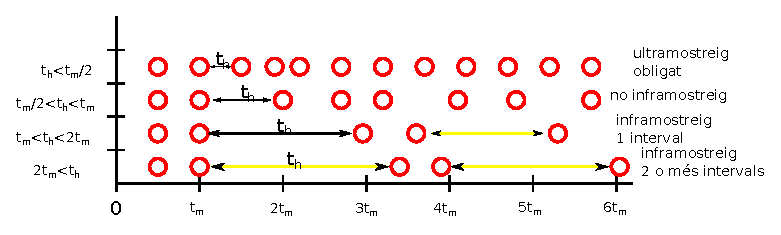
\includegraphics[width=\textwidth]{imatges/rrdtool/terminis.eps}
  \caption{Comparació de mostrejos amb terminis $t_h$ diferents pel mateix període de mostreig $t_m$, punts de mesura en vermell i intervals inframostrejats en groc}
  \label{fig:rrdtool:terminis}
\end{figure}

Primer de tot, del concepte de RRDtool es desprèn que en qualsevol cas sempre hi pot haver ultramostreig. Això és degut a que els terminis són els temps màxims entre mesures però no s'especifica un temps mínim. Aquestes situacions es poden veure a la figura~\ref{fig:rrdtool:terminis}: a l'eix horitzontal hi ha marcats els temps de mostreig exactes però el temps de mesura pot prendre qualsevol valor mentre sigui inferior al termini prefixat.


Un termini més gran que el temps de mostreig  ($t_h>t_m$) indica que s'accepten els casos d'inframostreig i el temps del termini limita el temps durant el qual es permet no disposar de mesures. A més, si el termini és més petit que el doble del temps de mostreig ($t_m<t_h<2t_m$), com a màxim només hi pot haver un interval amb inframostreig. Però si el termini supera el doble del temps de mostreig, llavors l'inframostreig es pot donar en dos intervals, en tres intervals si és el triple, etc.

Un termini més petit que el temps de mostreig ($t_h<t_m$) indica que no es vol inframostreig; és a dir que en cada interval com a mínim hi ha d'haver una mostra. Però, al mateix temps, un termini més petit que el temps de mostreig fa que a la llarga s'obligui a ultramostrejos en alguns intervals. Encara més, si el termini és inferior a la meitat del temps de mostreig, llavors hi ha d'haver ultramostreig en tots els intervals.

Normalment, en els usos de RRDtool, el valor del termini s'assigna a un valor més gran que el doble del temps de mostreig ($t_h>2t_m$) per tal de poder tenir folgança en les mesures. Cal observar que el cas del mostreig únic es representa amb el termini doblant el temps de mostreig ($t_h=2t_m$); això permet que la mesura següent se situi en qualsevol temps de l'interval de mostreig següent.

El cas del mostreig únic és comparable als sistemes en temps real. En els sistemes en temps real el temps entre mostres com a màxim pot doblar el temps de mostreig, mentre es compleixi que en cada interval de mostreig hi ha una mostra. En el cas de RRDtool, quan $t_h=2t_m$, hi pot haver inframostreig i per tant es pot no complir el temps real requerit pel mostreig únic. 
En conclusió, el temps de termini a RRDtool només s'utilitza per avaluar si les dades són 'fresques', la responsabilitat de les mesures i del temps real recau a la part d'adquisició de dades dels sistemes de monitoratge. 

A RRD el termini es defineix a l'hora de crear una base de dades però es pot tornar a configurar. Cada variable mesurada (cada registre) té el seu termini.


\paragraph{Exemple} Ara es crea la base de dades velocitat.rrd amb un temps de mostreig de 10 segons i un termini de 6 segons.

\begin{lstlisting}[style=sh]
rrdtool create velocitat.rrd --start 1262304000 --step 10 \
        DS:mps:GAUGE:6:-U:U                             \
        RRA:AVERAGE:0.5:1:24                                 
\end{lstlisting}

S'actualitza la base de dades amb els valors $x=[1,1,1]$ en els temps $t=[6,10,20]$.

\begin{lstlisting}[style=sh]
rrdtool update velocitat.rrd 1262304006:1 1262304010:1 1262304020:1 
\end{lstlisting}

A continuació es mostren els valors emmagatzemats:
\begin{lstlisting}
00:00:00 UTC  --> <row><v>NaN</v></row>
00:00:10 UTC  --> <row><v>1.0000000000e+00</v></row>
00:00:20 UTC  --> <row><v>NaN</v></row>
\end{lstlisting}

Les mesures implicades en el primer interval [0,10] han complert els terminis ja que el temps entre mesures és igual o inferior a 6 segons. Però en el segon interval [10,20], l'última mesura dista 10 segons respecte de l'anterior i per tant s'ignora i es considera desconeguda. 


\subsubsection{Límits}

Una altra comprovació que es fa a les mesures és si estan dins d'un rang. A RRDtool es comprova que el valor mesurat és més gran que un límit inferior i que és més petit que un límit superior. Si la mesura està fora de rang, s'ignora i es considera desconeguda.
$$
x(t_i) > L_{\max}  \longrightarrow   x(t_i) = unknown 
$$
$$
x(t_i) < L_{\min} \longrightarrow   x(t_i) = unknown 
$$

El límits sempre es calculen a les mesures un cop ja han passat l'etapa de transformació a velocitat. En el cas dels comptadors es comprova que la velocitat calculada estigui dins del rang però no es comprova la magnitud comptada, és a dir el valor que realment s'ha mesurat.

A RRDtool els límits es defineixen a l'hora de crear una base de dades però es poden tornar a configurar. Cada variable mesurada, això és cada registre, té el seus límits. Si no es vol comprovar el rang de les mesures, els límits es poden configurar amb el valor desconegut (\emph{U}) per tal que no es tinguin en compte. 


\paragraph{Exemple} Ara es crea la base de dades velocitat.rrd amb un límit inferior de 0 i un límit superior desconegut.

\begin{lstlisting}[style=sh]
rrdtool create velocitat.rrd --start 1262304000 --step 10 \
        DS:mps:GAUGE:600:0:U                             \
        RRA:AVERAGE:0.5:1:24                                 
\end{lstlisting}

Ara s'actualitza la base de dades amb els valors $x=[0,1000,-1]$ en els temps $t=[10,20,30]$.

\begin{lstlisting}[style=sh]
rrdtool update velocitat.rrd 1262304006:1 1262304010:1 1262304020:1 
\end{lstlisting}

A continuació es mostren els valors emmagatzemats:
\begin{lstlisting}
00:00:00 UTC  --> <row><v>NaN</v></row>
00:00:10 UTC  --> <row><v>0.0000000000e+00</v></row>
00:00:20 UTC  --> <row><v>1.0000000000e+03</v></row>
00:00:30 UTC  --> <row><v>NaN</v></row>
\end{lstlisting}

No hi ha límit superior però sí que n'hi ha d'inferior. En el temps 30 el valor és més petit que el límit i per tant s'ignora la mesura i es considera desconeguda.


\subsubsection{Càlcul amb dades desconegudes}

Fins ara s'ha vist les tres vies per on es poden obtenir dades desconegudes en la normalització d'intervals. Cal notar que les tres vies només serveixen per considerar si una mesura és desconeguda o no, però una mesura desconeguda no és suficient per considerar tot l'interval normalitzat desconegut.

A RRDtool, l'interval es considera desconegut\footnote{A l'etapa de normalització d'interval no es pot triar la quantitat de desconeguts que són acceptables, ni fins i tot poder decidir si un valor desconegut ja fa calcular tot l'interval com desconegut. A l'etapa de consolidació sí que és possible (v.\ secció~\ref{rrdtool:consolidacio:unknown}).}
quan el temps de mesures desconegudes ($T_u$)  és superior a la meitat del període de mostreig.
$$
T_u = \sum_{\forall x_f = unknown} ( t_f-t_{f-1} ) \quad
$$
$$
\text{si } T_u > t_m/2  \longrightarrow   x^N_{t^N_i} = unknown 
$$
sent $T_u$ el temps total que en un interval els valors $\mathbf{X}$ prenen valor desconegut.

En cas contrari es calcula l'interval amb els valors coneguts. És a dir, l'algoritme de normalització d'intervals ha de saber manipular les mostres amb mesures desconegudes. 
Per normalitzar, les dades desconegudes es considera que valen la mitjana de l'interval ($x_i^N=x_u$) .  D'aquesta manera no afecta a la velocitat mitjana de l'interval. Tot seguit es demostra.

\begin{figure}[tbp]
  \centering
  \begin{tikzpicture}
    \begin{axis}[
        width=10cm,scale only axis, height=5cm,
        xlabel=temps ,
        ylabel= valor,
        xticklabels={$\ldots$,,$t_{i-1}^N$,,$t_i^N$},
        ]
    \addplot[ycomb,blue] coordinates {
        (20,10)
        (30,10)
        (40,10)
    }; 
    \addlegendentry{}

    \addplot[ybar interval,yellow,fill=yellow!20!white] coordinates{
        (30,0)
        (30,10)
        (32,10)
        (32,0)
    };
    \addlegendentry{$t_a$}

   \addplot[ybar interval,purple,fill=purple!20!white] coordinates{
        (32,0)
        (32,10)
        (35,10)
        (35,0)
    };
    \addlegendentry{$t_{k-2}$}

    \addplot[ybar interval,orange,fill=orange!20!white] coordinates{
        (35,0)
        (35,10)
        (38,10)
        (38,0)
    };
    \addlegendentry{$t_0$}

    \addplot[ybar interval,green,fill=green!20!white] coordinates{
        (38,0)
        (38,10)
        (40,10)
        (40,0)
    };
    \addlegendentry{$t_b$}
 

 
    \addplot[only marks,mark=*,red] coordinates {
        (32,2)
        (35,3)
        (38,4)
        (45,2)
    };

    \node[below] at (axis cs:32,2) {$t_{T_f -k}$};
    \node[below] at (axis cs:35,3) {$\ldots$};
    \node[above] at (axis cs:38,4) {$t_{T_f -1}$};
    \node[above] at (axis cs:45,2) {$t_{T_f}$};



    \end{axis}
  \end{tikzpicture}
  \caption{Representació d'ultramostreig simplificada}
  \label{fig:rrdtool-etapes:desconeguts}
\end{figure}


Per una banda, la mitjana de l'interval sense tenir en compte els valors desconeguts es calcula utilitzant l'equació~\eqref{eq:rrdtool:ultramostreig} només en els valors coneguts. Per facilitar la comprensió, es reescriu l'equació utilitzant $t_a$, $t_b$ i $t_j$, representats a la figura~\ref{fig:rrdtool-etapes:desconeguts}:
$$%
t_a =t_{T_f-k}-t^N_{i-1} \quad\text{ i }\quad t_b = t^N_i-t_{T_f-1}
$$
$$
t_j =t_{T_f-1-j}-t_{T_f-2-j} \quad\forall j=[0,k-2]
$$
\begin{equation}\label{eq:rrdtool:normalitzacio}
x^N_i = \frac{t_ax_a+\sum\limits_{j=0}^{k-2} (t_jx_j)+t_bx_b}{t_a+\sum\limits_{j=0}^{k-2} (t_j)+t_b}
\end{equation}
Per altra banda, l'equació tenint en compte els valors desconeguts ($x_u$) és
\begin{equation}\label{eq:rrdtool:normalitzacio-desconegut}
x^N_i = \frac{t_ax_a+\sum\limits_0^{k-2} (t_jx_j)+t_bx_b+T_ux_u}{t_a+\sum\limits_0^{k-2} (t_j)+t_b+T_u}
\end{equation}
Substituint \eqref{eq:rrdtool:normalitzacio} a \eqref{eq:rrdtool:normalitzacio-desconegut} 
\[
x^N_i = \frac{ x_i^N(t_a+\sum\limits_0^{k-2} (t_j)+t_b)+T_ux_u}{t_a+\sum\limits_0^{k-2} (t_j)+t_b+T_u}
\]
operant amb aquesta expressió
\begin{align*}
 x^N_i - \frac{ x_i^N(t_a+\sum\limits_0^{k-2} (t_j)+t_b)+T_ux_u}{t_a+\sum\limits_0^{k-2} (t_j)+t_b+T_u} &= 0\\
 \frac{x^N_i(t_a+\sum\limits_0^{k-2} (t_j)+t_b+T_u) -  x_i^N(t_a+\sum\limits_0^{k-2} (t_j)+t_b)-T_ux_u}{t_a+\sum\limits_0^{k-2} (t_j)+t_b+T_u} &= 0\\
\frac{T_ux_i^N+T_ux_u}{t_a+\sum\limits_0^{k-2} (t_j)-t_b+T_u} &= 0
\end{align*}
Aleshores
\[
x_i^N = x_u
\]


Per tant si els valors desconeguts valen el mateix que la mitjana ($x_u=x^N_i$), aquesta mitjana es pot calcular senser tenir-los en compte com a l'equació~\ref{eq:rrdtool:normalitzacio}. En aquesta equació el temps de l'interval queda reduït, ja que el temps total de l'interval equival al temps de mostreig
$$
t_m= t_a+\sum\limits_0^{k-2} (t_j)+t_b+T_u
$$
i per tant es pot reexpressar a l'eq.~\ref{eq:rrdtool:normalitzacio} com el temps de mostreig descomptant-hi els temps en valors desconeguts
$$
t_a+\sum\limits_0^{k-2} (t_j)+t_b = t_m -T_u
$$

En resum, la normalització de l'interval es pot calcular amb l'àrea acumulada dels valors sense comptar-hi els desconeguts i al final dividida entre el temps de mostreig descomptant-hi els temps en valors desconeguts
$$
x^N_i = \frac{t_ax_a+\sum\limits_0^{k-2} (t_jx_j)+t_bx_b}{t_m - T_u}
\quad\forall\ x(t)\neq unknown
$$


Com que es dóna un valor al desconegut, això fa que la magnitud comptada augmenti. És a dir, s'està suposant que el comptador ha seguit mesurant a una velocitat semblant a les altres de l'interval.

Aquest augment s'observa seguint l'equació $e=x(t)$
$$
e_{mesurat} = x_at_a+\sum\limits_0^{k-2} (x_jt_j)+x_bt_b
$$
$$
e_{emmagatzemat} = x_at_a+\sum\limits_0^{k-2} (x_jt_j)+x_bt_b+x^N_iT_u
$$



% Atenció: sembla que hi ha un bug

% Heartbeat=600. Mentre que 
% rrdtool updatev consolida.rrd 1262304015:1 1262304030:U dóna 1(?),1(no) updatev consolida.rrd 1262304015:1 1262304029:U 1262304030:U dóna 1(bé),U(bé)

% però si Heartbeat=12 dóna U,U


% Un altre bug. Heartbeat=3 rrdtool updatev consolida.rrd 1262304013:1 1262304016:1 1262304019:1 1262304022:1 dóna 1(bé). rrdtool updatev consolida.rrd 1262304013:1 1262304017:1 1262304020:1 dóna 1(bé). però rdtool updatev consolida.rrd 1262304013:1 1262304016:1 1262304020:1 dóna U(no)

% %http://www.vandenbogaerdt.nl/rrdtool/total.php
% %http://www.mrtg.org/rrdtool/doc/rrdcreate.en.html



\subsection{Algoritme de normalització}
Ara es modifica l'algoritme tenint compte les dades desconegudes i també els ultramostrejos i inframostrejos dels intervals. Aquest és l'algoritme complet de normalització d'intervals.



\begin{lstlisting}[mathescape=true]
Normalització d'una sèrie temporal
a períodes de mostreig regulars 
INPUT: 
      vector de valors $\mathbf{X} = [x_0,x_1,\ldots,x_f]$ 
      vector de temps $\mathbf{T} = [t_0,t_1,\ldots,t_f]$
      període de mostreig regular  $t_m$
      termini $H$
      llindars màxim $X^{MAX}$ i mínim $X^{MIN}$
OUTPUT: 
      vector de valors normalitzats $\mathbf{X^N} = [x_0^N,x_1^N,\ldots,x_k^N]$

$x_0^N$ := unknown <-- primer valor normalitzat desconegut
$t^N$ := $t_m$ <-- següent interval de normalització
i := 1

$A$ := 0 <--- àrea acumulada
$t_{ant}$ := 0 <-- temps de la mostra anterior
$T_u$ := 0 <-- temps en valor desconegut

per cada parella $(x,t)$ en $\mathbf{X}$ i $\mathbf{T}$ fes:

    avalua termini i llindar:
    si $t-t_{ant}$ > $H$ o no $X^{MIN}$ $\leq$ x $\leq$ $X^{MAX}$ llavors x:= unknown fsi

    si $t < t^N$ llavors
        si x = unknown llavors
            $T_u$ := $T_u + t -t_{ant}$ <-- acumula temps desconegut
        sino
            $A$ := $A + x( t-t_{ant} )$ <-- acumula valor
        fsi

    sino  <-- càlcul d'un valor normalitzat

        $N_{inf}$ := $(t-t^N)$ div $t_m$ <-- n. d'intervals amb inframostreig

        si x = unknown llavors
            $T_u$ := $T_u+t^N -t_{ant} +N_{inf}\cdot t_m$ <-- acumula temps desconegut
        sino
            $x_i^N$ := $A + x( t^N-t_{ant} ) + x \cdot N_{inf} \cdot t_m$ <-- acumula valor
        fsi

        si $T_u > \frac{(1+N_{inf})t_m}{2}$ llavors
            $x_i^N$ := unknown <--  normalitza desconegut
        sino
            $x_i^N$ := $\dfrac{A}{t_m (1+N_{inf})-T_u}$ <--  normalitza valor
        fsi

        mateix valor per cada interval amb inframostreig
        $x_{i+N_{inf}}^N$ := $\,\cdots\,$ := $x_{i+1}^N$ := $x_i^N$
                
        si x = unknown llavors <-- acumula desconegut, reset àrea 
            $T_u$ := $t-t_{ant}$
            $A$ := 0
        sino <-- acumula àrea, reset desconeguts
            $T_u$ := 0
            $A$ := $x( t-t^N )$
        fsi

        $t^N$ := $t^N + (N_{inf}+1) t_m$ <-- següent interval de normalització
        i := i + ($N_{inf}$+1)

    fsi 

    $t_{ant}$ := $t$

repeteix
\end{lstlisting}




\section[Consolidació]{Consolidació d'intervals}

Un cop s'ha normalitzat l'interval, a la base de dades hi ha els valors amb temps de mostreig regular (\emph{step}). Aquest valors ja normalitzats a RRDtool s'anomenen \emph{Primary Data Points} (PDP). 

Però aquest interval de mostreig inicial no es pot mantenir durant gaire temps ja que cada cop és més difícil gestionar la quantitat de dades. Per afitar la quantitat de dades emmagatzemades, RRDtool desa les dades en diferents resolucions temporals. 

És a dir, cal consolidar l'interval normalitzat inicial a altres temps de mostreig desitjats. A partir dels PDP es tornen a mostrejar (\emph{resampling}) nous intervals amb menys resolució. 

A RRDtool, aquest valors nous consolidats s'anomenen \emph{Consolidated Data Points} (CDP) i cada resolució s'emmagatzema en les taules anomenades \emph{Round Robin Archive} (RRA).
Cada CDP es calcula a partir de $n$ PDP i cada RRA defineix aquest $n$ necessari, el qual a RRDtool s'anomena \emph{step} però que cal no confondre'l amb l'\emph{step} de normalització d'interval. Es poden distingir com a \emph{step de CDP} i \emph{step de PDP}, respectivament.


En aquest càlcul pot interessar conservar diferent informació de les variables mesurades. El canvi de resolució implica una pèrdua de precisió i informació, cal trobar un càlcul que mantingui les propietats que interessin de les dades

Per un RRA que aplica una funció $f$ de consolidació a $n$ PDP (valors normalitzats $V^N$) per obtenir un CDP:
$$
CDP_i = f(x^N_{i-n},\ldots,x^N_i) \qquad i \in \{ n,2n,3n\ldots \}
$$

És a dir que la resolució dels CDP sempre és múltiple del temps de mostreig base dels PDP. 
Actualment RRDTool permet calcular quatre funcions de consolidació: 

\begin{itemize}
\item mitjana (AVERAGE)
\item màxim (MAX)
\item mínim (MIN)
\item últim (LAST)
\end{itemize}

% Aquestes funcions tenen la particularitat que es poden calcular de manera incremental.
% $$
% CDP_i =   f(f( \ldots( f(f(unknown,x^N_{i-n}), x^N_{i-n+1}),\ldots ), x^N_{i-1}) ,x^N_i )  \qquad i \in \{ n,2n,3n\ldots \}
% $$


Calcular la mitjana és equivalent al que es fa a l'etapa de normalització de l'interval. En aquell cas cal fer una mitjana ponderada per la durada de la mesura però ara els intervals són iguals per tots els valors i per tant ja no cal considerar el temps. 
$$
\text{CDP}_i(\text{AVERAGE}) = \frac{\sum\limits_{k=1}^N t_m\text{PDP}_k }{\sum\limits_{k=1}^N t_m}
= \frac{t_m\sum\limits_{k=1}^N \text{PDP}_k}{nt_m}
= \frac{\sum\limits_{k=1}^N \text{PDP}_k}{n}
$$
on $n$ és el total de valors normaitzats que s'agafen, el qual s'ha anomenat \emph{step de CDP}.

Per als càlculs de màxim, mínim i últim cal recordar que s'apliquen als PDP, és a dir un cop els valors mesurats han estat normalitzats. Per exemple en el cas del màxim no es conserva el valor més alt que s'ha mesurat sinó el valor més alt dels PDP; un cop s'ha fet la mitjana ponderada de les mesures. 

Una altra lectura possible és que en un RRA que calculi cada CDP amb un PDP tant és quina funció s'apliqui; els CDP seran iguals als PDP.

\subsection{Dades deconegudes}\label{rrdtool:consolidacio:unknown}

A la sortida de l'etapa de normalització, alguns intervals poden prendre el valor 'desconegut' (\emph{unknown}). Les funcions de consolidació han de calcular amb aquests valors i per tant han de decidir com tractar-los.

Per una banda, quan l'etapa de normalització es troba valors desconeguts en un interval de mostreig, aproximació la normalització de manera que els valors desconeguts no alterin la mitjana dels valors coneguts. 
Ara a l'etapa de consolidació també s'aplica el mateix criteri per a la funció de consolidació de mitjana: com s'ha fet per $x_u=x_i^N$ a  \eqref{eq:rrdtool:normalitzacio} a \eqref{eq:rrdtool:normalitzacio-desconegut} ara s'aplica el mateix a $x_U=\text{CDP}_i$ i aleshores es pot escriure
$$
\text{CDP}_i(\text{AVERAGE}) = \frac{\sum\limits_{k=1}^N \text{PDP}_k}{n_{\text{coneguts}}} = \frac{x_u+\sum\limits_{k=1}^N \text{PDP}_k }{n}
$$


Però hi ha altres funcions i cal generalitzar el criteri. Per a les funcions de mínim i màxim es considera que els valors desconeguts no afecten en el càlcul i per a la funció d'últim el valor consolidat pren el que calgui, valor o 'desconegut'. Per tant, aquestes funcions no es veuen afectades per $n$.

Per altra banda, a l'etapa de normalització es considera un interval desconegut quan més de la meitat de l'interval de mostreig té valors desconeguts. 
Però ara, a l'etapa de consolidació, hi ha un paràmetre que permet decidir el percentatge de valors desconeguts que calen perquè el valor consolidat sigui considerat desconegut. Aquest paràmetre s'anomena xff (\emph{xfiles factor}\footnote{RRDtool l'anomena el factor d'expedients X (\emph{X-Files Factor}) perquè si té un valor diferent de zero el resultat està fora dels límits científics,~\cite{vandenbogaerdt}}).
$$
N_{\text{desconeguts}}/N > \text{xff} \longrightarrow \text{CDP}_i = unknown
$$
on l'xff s'expressa en tant per u. 

A continuació es resumeix el tractament de desconeguts en un algoritme
\begin{lstlisting}[mathescape=true]
Consolidació d'una sèrie temporal
cada període de consolidació segons els valors normalitzats
INPUT: 
      vector de valors normalitzats $\mathbf{PDP} = \mathbf{X^N} = [x_0^N,x_1^N,\ldots,x_k^N]$
      funció d'interpolació $f$
      període de consolidació  $N$ en n. de PDP
      llindar de desconeguts $x^{ff}$ en tant per u
OUTPUT: 
      vector de valors consolidats $\mathbf{CDP} = [cdp_0,cdp_1,\ldots,cdp_l]$

i := 0
$cdp_i$ := unknown

$a$ := 0 <-- acumulador pels interpoladors
$T_u$ := 0 <-- Temps en valor desconegut
$n$ := 1 <-- quantitat de PDP calculats

per cada $p$ a $\mathbf{PDP}$ fes:

    si $p$ = unknow llavors
        $T_U$ := $T_u + 1$ <-- acumula temps desconegut
    
    sino <-- aplica l'interpolador corresponent
        cas f és
            AVERAGE $\longrightarrow$ $a$ := $\dfrac{a(n-1) + p}{n}$  
            MAX $\longrightarrow$ $a$ := $\max(a, p)$  
            MIN $\longrightarrow$ $a$ := $\min(a, p)$  
            LAST $\longrightarrow$ $a$ := $p$  
        fcas
    fsi

    si $n = N$ llavors <-- consolida

        si $T_u$ / N > $x^{ff}$ llavors
            $cdp_i$ := unknown <-- consolida desconegut
        sino
            $cdp_i$ ::= acumulat <-- consolida el valor
        fsi
        i := i+1 
        $n$ := 0
        $a$ := 0
        $T_u$ := 0
    fsi
    n := n + 1
repeteix
\end{lstlisting}






%%% Local Variables:
%%% TeX-master: "memoria"
%%% End:

% LocalWords:  RRDtool RRD Gauge width rrd UTC row NaN Counter Absolute



\section{Time series model}
\label{sec:model:TSMS}

Following current database models, a \acro{TSMS} model consists of two
components: a data model and a set of operations. \emph{Measures} and
\emph{time series} are the main objects of our \acro{TSMS} model.
%
In this section we describe and formalise the \acro{TSMS} model. 


\subsection{Data model}

Roughly speaking a \emph{time series} is a set of observations
collected at specific time instants. An observation may consist of
single value or multiple values collected at the same time instant.
Each pair of time and observed values is referred to as a
\emph{measure}. Then, a time series is a correspondence between times
and values. A time series can be described by a set of measures.

We name \emph{time domain} the set $\cal{T}$ of all the possible time
values. $\cal{T}$ can be either a finite or an infinite set and
usually it is a closed set. Although time is a complex issue
\cite{iep:time-supplement}, in this paper we will assume that the
$\cal{T}$ is the set of affinely extended real numbers $\Rb = \R \cup
\{+\infty,-\infty\}$. This avoids the complex details of time
modelling while being powerful enough for our purposes. Next, we
define the main time related concepts using this naive approximation.



\begin{definition}[Time concepts]
  \label{def:model:temps}
  Let $\cal{T}=\Rb$ be the domain for time.
  %
  We name an element $t\in\cal{T}$ as \emph{time instant}.
  %
  Let $s,t\in\cal{T}$ be two time instants.  We define the
  \emph{duration of time} between $s$ and $t$ as the value $d
  \in\cal{T}$ which measures the distance in time units between the
  two time instants, that is $d =|s-t|$.
\end{definition}

The \emph{value} is an attribute that indicates the magnitude of a
measure. The domain for the values can be any data type. Valid domains
for values include integers, real numbers, strings, and more
elaborated data structures such as arrays, lists, or even other time
series. Here below, the domain for values will be denoted by
$\cal{V}$. 
%
Without loss of generality in this paper we will assume that the
domain of values is the set of projectively extended reals $\Rp = \R
\cup \{\infty\}$.

A measure represents an actual value measured in a particular time
instant. We define it below.

\begin{definition}[Measure]
  Let $v\in\cal{V}$ be a value and let $t\in\cal{T}$ be the time
  instant when the value was acquired. We define a \emph{measure} $m$
  as the tuple $m=(t,v)$. The domain of a measure $m$, written as
  $\dom m$, is the domain of its value.
\end{definition}

Let $m = (t,v)$ be a measure. In what follows, $V(m)$ denotes the
value $v$ and $T(m)$ denotes the time $t$.

Order between measures plays an important role. Given two measures we
define two distinct \emph{order relations}.

\begin{definition}[Semitemporal order]\label{def:semitemporal_order}
  Let $m$ and $n$ be two measures. We name \emph{semitemporal order}
  the binary relation written $m\leq n$, defined as $m\leq n\iff
  (T(m)<T(n) \vee ( T(m)=T(n) \wedge V(m) = V(n) ))$.
\end{definition}

\begin{definition}[Temporal order]\label{def:temporal_order}
  Let $m$ and $n$ be two measures. We
    name \emph{temporal order} the binary relation written $m \leq^t
    n$ and defined as $m \leq^t n \iff T(m) \leq T(n)$.
\end{definition}

Note that the semitemporal order is a partial order while the temporal
order is a total order.

Intuitively speaking a \emph{time series} is a ordered set of measures of the
same phenomena.  Sometimes they are also called \emph{time
sequences}~\cite{last:hetland}. We define it as follows.

\begin{definition}[Time series]
  \label{def:model:timeseries}
  Let $S = \{m_0,\ldots,m_k\}\subset\cal{T}\times\cal{V}$ be a finite
  set of measures of the same type. Then, $S$ is a \emph{time series}
  iff $\forall i,j: i,j\in[0,k] \wedge i\neq j: T(m_i)\neq T(m_j)$.
  We define the domain of a time series $S$, denoted as $\dom S$, as
  the domain of its measures.
\end{definition}

Observe that although measures in $S$ are expected to be of the same
phenomena, from a formal standpoint we only require the domain of all
values to be the same. 

In a time series there are not two measures with the same time. Thus,
considering the temporal order, a time series is a totally ordered
set.

The \emph{cardinality} of a time series $S=\{m_0,\dots,m_k\}$, noted as
$|S|$, is the number of measures that contains.  An \emph{empty time series} is
noted as $\emptyset$. Needless to say, $|\emptyset|=0$.

Although we defined values as scalars, it is easy to extend the
concept. Following~\cite{assfalg08:thesis}, a time series can record
more than one phenomena if they share the same acquisition time
instants.  This kind of series are known as \emph{multivalued time
  series}. Let $S$ be a multivalued time series and let its domain be
$\dom S={\cal{V}}_1\times\cdots\times{\cal{V}}_n$. Then, we write its
measures as $m=(t,v_1,v_2,\ldots,v_n)$.



A time series is \emph{regular} when its measures are equi-spaced in time,
according to \cite{last:hetland}.  Let $S=\{m_0, m_1,\ldots,
m_{k-1},m_k\}$ be a time series, where
$T(m_0)<T(m_1)<\dots<T(m_{k-1})<T(m_k)$, and let $d\in\cal{T}$ be a
time duration. Then $S$ is \emph{regular} when $d=T(m_1)-T(m_0)=
\dots =T(m_k)-T(m_{k-1})$.




\subsection{Operations}
\label{sec:model:operations}

Time series can be manipulated through the operations defined in this
section.
%
Like the relational model operations, operations over time series
ignore the actual semantics of the data. In a particular application,
it should be decided whether an operation is semantically coherent or
must not be applied. For example, the addition of values coming from two
different phenomena could be semantically erroneous.

In this section three groups of operations are formalised, one in each
of the subsections which follow. The set operations, that consider
times series as sets; the sequence operations, that consider time
series as sequences; and the temporal operations, that manipulate the
time series assuming that are representations of functions.



\subsubsection{Set operations}
\label{sec:set}

We describe how common set operators can be applied to time series. We
rely on how the relational model of \acro{DBMS} describes operations
based on set algebra~\cite{date:introduction}.

Consider a time series $S$. $S$ is a finite ordered set (by the
temporal order). Then, if $S$ nonempty, $S$ has a maximum and a
minimum.  
%
The \emph{maximum}
of $S$, denoted as $\max S$, is an element of $S$ such that $\forall m
\in S:\max S\geq^t m $.  
%
Note that $\max S$ is not defined when $S=\emptyset$. However, the
time series has a supremum even when empty. In fact, according
to~\cite{cantrell:extendedreal}, $\sup \emptyset=-\infty$.
%
Let $m=(-\infty,\infty)$ be a measure with infinite time and value.
Using this fact we define the \emph{supremum} of $S$, noted as
$\sup S$, as
\[
\sup S =\begin{cases}
  \max S    & \text{when $S$ nonempty}\\
  m   & \text{otherwise}
\end{cases}
\]
Dually, we can define the \emph{minimum} of $S$, noted as $\min S$,
and the \emph{infimum} of $S$, noted as $\inf S$.

The \emph{membership} operation defines when a measure belongs to a time
series. We define two distinct membership operations which consider
the semitemporal order (Definition~\ref{def:semitemporal_order}) and
the temporal order (Definition~\ref{def:temporal_order}). In
consequence, they induce two different ways to consider time series
and its operations.

Let $S$ be a time series and $m$ be a measure. 
%
We say that $m$ belongs to $S$ (plain \emph{membership}), denoted as
$m \in S$, when $\exists x\in S: x=m$.  We also say that $m$ belongs
temporally to $S$ (\emph{temporal membership}), denoted as $m \inst
S$, when $\exists x\in S : T(m)=T(x)$.


The two distinct membership criteria induce two meanings for
inclusion. Let $R$ and $S$ be two time series.  We say that $R$ is
\emph{included} in $S$, written $R\subseteq S$, when all the elements
of $R$ belong to $S$.  Analogously, we say that $R$ is \emph{included
  temporally} in $S$, noted $R\subseteqt S$, when all the elements of
$R$ belong temporally to $S$.


The \emph{union} of two sets is a set containing elements from both
sets. Usual set union operations do not apply to time series because
the result time series could have repeated time values.  Thus, we 
give a slightly modified concept for union.

The union operation requires both time series to have the same domain,
as is also true with the union operation of relational
algebra~\cite{date:introduction}.

Let $R$ and $S$ be two time series and let $\dom R =\dom S$. 
%
The \emph{union} of $R$ and $S$, noted $R\cup S$, is a new time series
$R \cup S = \{m|m\in R\vee (m\in S\wedge m \notinst R)\}$. 
%
The \emph{temporal union} of $R$ and $S$, noted $S_1 \cupt S_2$, is a
time series $R \cupt S = \{ m | (m \in R \wedge m \in S) \vee (m \in R
\wedge m \notinst S) \vee (m \in S \wedge m \notinst R) \}$.  
%
It is interesting to emphasise that the union is a non commutative
operation while the temporal union is a commutative one.

\begin{figure}
  \centering
  %\def\escala{0.9}

\def\nodeA{node [above left=0.5cm and 0.1cm] {$(1,1)$} node [below left=0.5cm and 0.1cm] {$(5,1)$}}
\def\nodeB{node [above right=0.5cm and 0.1cm] {$(2,2)$} node [below right=0.5cm and 0.1cm] {$(6,2)$}}
\def\nodeT{node [above=0.1cm] {$(4,0)$} node [left=0.4cm] {$(3,1)$} node [right=0.4cm] {$(3,2)$}}
% Definition of circles
\def\firstcircle{(0,0) circle (1.5cm)}
\def\secondcircle{(0:2cm) circle (1.5cm)}
\def\thirdcircle{(0:1cm) circle (1.11cm)}

\colorlet{circle edge}{blue!50}
\colorlet{circle area}{blue!20}

\tikzset{
  filled/.style={fill=circle area, draw=circle edge, thick},
  outline/.style={draw=circle edge, thick},
  every node/.style={transform shape}
}

%\setlength{\parskip}{5mm}






%Set A or B
\begin{tikzpicture}[scale=\escala]
  \draw[filled] \firstcircle \nodeA;
    \begin{scope}
        \clip \secondcircle;
        \draw[filled, even odd rule] \firstcircle \nodeA
                                 \secondcircle 
                                 \thirdcircle;
   \end{scope}
    \draw[outline] \firstcircle
                   \secondcircle \nodeB
                   \thirdcircle \nodeT;

   \node[anchor=south] at (current bounding box.north) {$S_1 \cup S_2$};
\end{tikzpicture}
%Set temporal A or B
\begin{tikzpicture}[scale=\escala]
    \draw[filled, even odd rule] \firstcircle \nodeA
                                 \secondcircle \nodeB
                                 \thirdcircle \nodeT;
    \node[anchor=south] at (current bounding box.north) {$S_1 \cup^t S_2$};
\end{tikzpicture}






%%% Local Variables:
%%% TeX-master: "../main"
%%% ispell-local-dictionary: "british"
%%% End:

  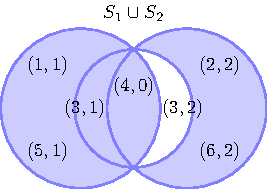
\includegraphics{fig_model_venn.pdf}
  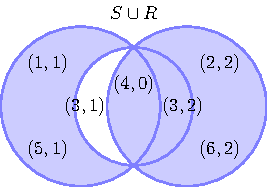
\includegraphics{fig_model_venn_reverse.pdf}
  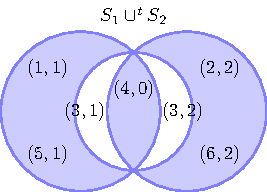
\includegraphics{fig_model_venn2.pdf}
  \caption{Venn diagrams for set and temporal set union operations of
    \acro{TSMS}}
  \label{fig:model:venn}
\end{figure}


\begin{example}\label{ex:model:s1s2}
  Let $R=\{(1,1), (3,1), (4,0), (5,1)\}$ and $S=\{(2,2), (3,2), (4,0),
  (6,2)\}$ be two time series. The union of $R$ and $S$ is $R\cup
  S=\{(1,1), (2,2), (3,1), (4,0), (5,1), (6,2)\}$. Because union is
  not symmetric, $S\cup R=\{(1,1), (2,2), \allowbreak(3,2), (4, 0), (5,1),
  (6,2)\}$. The temporal union results in $R\cupt S= S \cupt
  R=\{(1,1), (2,2), (4,0), (5,1), (6,2)\}$.  
  %
  Venn diagrams for all three cases are shown in
  Figure~\ref{fig:model:venn}, where the coloured area depicts the
  result time series. In every diagram, the central intersection area
  contains measures that share both time and value attributes, like
  instance $(4,0)$. The central left area contains the measures in $R$
  that only share the time attribute with a measure in $S$, like
  instance $(3,1)$. The central right area has a symmetrical
  meaning. The left and right outer areas are the remaining measures
  of $R$ and $S$ respectively.
\end{example}




Time series \emph{difference} can also be defined. Like union, the
difference requires both time series to have the same domain.
%
Let $R$ and $S$ be two time series and let $\dom R = \dom S$.
%
The \emph{difference} between $R$ and $S$, written $R-S$, is a time
series $R-S=\{m|m\in R\wedge m\notin S\}$.
%
The \emph{temporal difference} between $R$ and $S$, denoted $R-^t S$, 
is a time series $R-^t S=\{m|m\in R\wedge m \notinst S\}$.


Based on union and difference we can define \emph{intersection} as
$R\cap S = R - (R - S)$ and \emph{symmetric difference}
as $R \ominus S = (R - S) \cup (S - R)$. The
corresponding temporal operations can also be defined.


Relational \acro{DBMS} extend the set operators by some more such as
selection, rename or join. This kind of operators also make sense for
time series. To illustrate this possibility we define the join
operator.

Roughly speaking, the join of two time series is the combination of
measures sharing the same time attribute.  Let $R$ and $S$ be two time
series.  The \emph{join} of $R$ and $S$, denoted $R \join S$, is a
multivalued time series $R \join S = \{ (t,v_1,v_2) | (t,v_1) \in
R\wedge (t,v_2) \in S\}$. Note that $\dom(R\join
S)=\dom R\times\dom S$.
%
It must be noted that join requires both time series measures to share
exactly the same times. When time series diverge, the temporal
function operations explained later can be applied to adjust the time
instants to join requirements.


A \acro{DBMS} requires computational operators to provide opportunity
to calculate using the data contained. Relational \acro{DBMS} supply
operators like extend, aggregate or
summarise~\cite{date:introduction}. For time series, we define the more
general computational operators \emph{map} and \emph{fold}.

The map operator transforms a time series $S$ into a new time series
$R$ by applying a function to every measure.  Let $S$ and $R$ be two
time series, let $\cal{V}=\dom S$ and $\cal{V'}=\dom R$, and let
$f:\cal{T}\times\cal{V}\rightarrow\cal{T}\times\cal{V'}$ be a function
over a measure returning a measure. The \emph{map} of $f$ over $S$ is
a new time series defined as $\map(S,f)=\{f(m)|m\in S\}$. Note that
$\dom(\map(S,f))=\cal{V'}$.
%


The fold operator recursively combines every measure of a time
series. Assuming that $\mathcal{P}(C)$ is the powerset of $C$, we
define fold as follows.
%
Let $S=\{m_0,\dots, m_k\}$ and $R$ be two time series, let
$\mathcal{V}=\dom S$, let $\mathcal{V'}=\dom R$ and let 
%
$f:\mathcal{P}(\mathcal{T}\times\mathcal{V'}) \times (\mathcal{T}\times\mathcal{V}) \rightarrow \mathcal{P}(\mathcal{T}\times\mathcal{V'})$ 
%
be a function over a time series and a measure, which returns a time
series.
%
The \emph{fold} of $S$ by $f$ with initial value $R$ is a new time
series defined as $\fold(S,R,f) = f(\cdots(f(f(f(R,m_0),\allowbreak
m_1),\allowbreak m_2)\cdots),\allowbreak m_k)$.
%



The classical aggregation operator combines the data of a time series
into a single value.  It is worth to note that it is a special
case of fold.

Let $S=\{m_0,\dots,m_k\}$ be a time series, let $\mathcal{V}=\dom S$,
let $m$ be a measure with $\dom m=\mathcal{V}$, and let 
%
$f:(\mathcal{T}\times\mathcal{V})\times(\mathcal{T}\times\mathcal{V})\rightarrow \mathcal{T}\times\mathcal{V}$ 
%
be a function over two measures returning a measure. The
\emph{aggregate} of $S$ by $f$ with initial value $m$ is a new time
series defined as $\agg(S,m,f) = f(\cdots(f(f(f(m,m_0),\allowbreak
m_1),\allowbreak m_2)\cdots),\allowbreak m_k)$.  

% In the previous fold, the measures are computed in random order.
% However in some computational operations it is necessary to define the
% order, especially when $f$ is not commutative.  Then, it is possible
% to define a \emph{fold with order} as an extension of fold where
% measures are computed in a predetermined order.

% We define a
% \emph{fold with order}, $\orderfold$, as an extension of fold with a
% function $o$ that selects measures in order where $o: S_a \mapsto m_r$
% \[
%  \orderfold(S,S_i,f^f,o) =
%   \begin{cases}
%     S_i  \text{ if } |S|=0, \\
%     \orderfold(S_o,f^f(S_i,m_o),f^f,o)  \text{ else}
%   \end{cases}
% \]
% where $m_o = o(S)$ and $S_o = S - \{m_o\}$.



\begin{example}
\label{ex:computational-operators}
Let $S=\{(1,1),(2,3),(4,1)\}$ be a time series.  Map operator allows
computing a new time series whose values result from time multiplied
by value.  We define the map function $f(t,v)=(t,t\cdot v)$. Then
$\map(S,f)=\{(1,1),(2,6),(4,4)\}$.  
%


The aggregate operator allows, for instance, to compute the measure
that results from the sum of all the values.  To illustrate it, we
define the aggregate function $f(m,n)=(0,V(m)+V(n))$. Now,
$\agg(S,(0,0),f) = (0,5)$, where $5$ is the sum of all the values of
$S$. Note that time is meaningless in this computation.

The fold operator allows, for instance, to select the measures having
its value equal to one.  We define the fold function $f(R,m)=R\cup R'$
where $R'=\{m\}$ if $V(m)=1$ or $R'=\emptyset$ otherwise. Let $m$ be
any measure, note that $f(\emptyset,m)= R'$. Then
$\fold(S,\emptyset,f)=\{(1,1),(4,1)\}$.
\end{example}

%%%%%%% BINARY COMPUTATIONAL OPERATORS

Finally we describe how, using the operators defined before, we can
implement \emph{binary computational} operators between two time
series. This illustrates the power of the operators defined so far.
%

The strategy requires first to join the two time series and then
apply the computational operations. 
%
Let $S$ and $R$ be two time series and $\odot$ be a binary operator on
the value domain. The operator $\odot$ can be extended to the time
series as:
%
$S\odot R=\map(S\join R, f)$ being $f$ the function
$f(t,v,w)=(t,v\odot w)$.
%
This allows to extend real binary operations such as sum, $R+S$, or
division, $R/S$, to time series.


\subsubsection{Sequence operations}
\label{sec:sequence}

Sequence operations manipulate time series considering measures as
being totally ordered by time.  We define three basic operations:
\emph{slice}, \emph{successor} and \emph{concatenation}.


The classical interval concept can be applied to time domain. In this
context, given two time instants $s$ and $t$, we use the notation
$[s:t]$, $(s:t)$, $[s:t)$ and $(s:t]$ respectively for the closed
interval, open interval, open right and open left interval.
%
Following~\cite{last:hetland}, to slice a time series $S$ means to
extract a new time series $R\subseteq S$ constrained to a given time
interval. We denote this operation as the original time series followed
by the interval. Therefore, $S[s:t]=\{m|m\in S \wedge
T(m)\in[s:t]\}$. We can use other intervals to slice a time series in
a same fashion. For instance, $S(s:t]=\{m|m\in S \wedge
T(m)\in(s:t]\}$.

The ordinary time order allows to define the concepts of successor and
predecessor for the measures of a time series.
%
Let $S=\{m_0,\ldots,m_k\}$ be a time series and $m$ be an arbitrary
measure.
%
We say that $m_i=\nex_S(m)$ is the \emph{next} measure to $m$ in $S$ if and
only if $m_i=\inf(S(T(m):+\infty])$.  
%
We also say that $m_i=\prev_S(m)$ is the \emph{previous} measure to
$m$ in $S$ if and only if $m_i=\sup(S[-\infty:T(m)))$. 
%
Infinite measures are obtained when next and previous are applied to
supremum and infimum measures respectively: $\nex_S(\sup
S)=(+\infty,\infty)$ and $\prev_S(\inf S)=(-\infty,\infty)$.

To concatenate two time series means to compute a new time series with
the measures of the first time series followed in time order by the
measures of the second one. 
%
The concatenation requires both time series to share the same domain.
Let $R$ and $S$ be two time series and let $\dom R=\dom S$. The
\emph{concatenation} of $R$ and $S$, denoted as $R||S$, is a time
series that contains all the measures of $R$ together with those of
$S$ that do not intersect with the time interval of $R$. That is,
$R||S= R\cup (S - S[T(\inf R):T(\sup R)])$.



\subsubsection{Temporal function operations}
\label{sec:model:tfunc}

A time series can be thought as discrete representation of an
(original) temporal function. In this section we devise some
operations that manage the time series according to this temporal
function standpoint.  
%

The graph of a function allows to obtain and interpret the
continuous nature of a time series, when the domain of time and value
attributes can be plotted then the graph is equivalent to a graphical
representation.  
%
Let $S$ be a time series and $\cal{T}$ the time domain. The \emph{graph} of
the time series $S$ is a set of ordered pairs $\graph S
=\{(t,S(t))|t\in \cal{T}\}$ where $S(t)$ is a \emph{temporal representation
function} for the time series.
%


Given a time series $S$, the \emph{temporal representation function}
$S(t)$ is a function along the variable $t$ in the domain of
time and the target in the domain of values.
%
In some sense, $S(t)$ can be thought as the original temporal function
from which $S$ was obtained.
%

There is not an unique way to obtain $S(t)$ for a given time series
$S$. Because of this, in temporal representation functions we will
introduce a superscript, say $r$, that shows the name $r$ of the
representation method used. Then, $S(t)^r$ means the representation
function of $S$ using method $r$. Below, we exemplify the
representation functions using two different methods based on impulse
and constant piecewise functions.


\begin{definition}[Dirac representation] 
  Dirac delta (\dd) is a method of representation based on the Dirac
  delta function. Let $S$ be a time series. We define $S(t)^\dd$ as
  the following \dd{} representation function:
  \[
  S(t)^\dd
  =  \begin{cases}
          V(m) & \text{if } \exists m\in S:t=T(m) \\
          0    & \text{otherwise}
  \end{cases}
  \]
\end{definition}

\begin{definition}[Zohe representation]
  Zero-order hold everted (\zohe{}) is a method of representation
  based on the \emph{zero-order hold} signal reconstruction method. It
  is a piecewise constant function built from left-continuous step
  functions.  Let $S$ be a time series. We define $S(t)^\zohe$ as the
  following representation function:
  \[
  S(t)^\zohe 
  = \begin{cases}
    V(m) & \text{if } \exists m\in S: t\in \big(T(\prev_S(m)):T(m)\big]\\
    0    & \text{if } t > T(\max(S)) 
  \end{cases}
  \]
\end{definition}




The concept of representation is used for formalising some set and
sequence operators as temporal operators. 

% Consequently, the result of each one will depend on a representation
% method, which is indicated as a parameter.


We define a temporal interval operation to introduce this concept.
Let $S$ be a time series, let $[s:t]$ be an interval of two time
instants and let $r$ be a representation method. The \emph{temporal
  interval}, denoted as $S[s:t]^r$, returns a new time series with
measures in the interval temporal range. That is, $S[s:t]^r = S(u)^r$
for all $u \in [s:t]$. This is a general definition difficult to
implement, so for every representation a particular temporal interval
must be interpreted:

\begin{itemize}
\item Let $S(t)^\dd$ be the \dd{} representation for $S$. The
  \emph{\dd{} temporal interval} is $S[s:t]^\dd = S[s:t]
  \cup \{m\} \cup \{n\}$ where $m=(s,0)$ and $n=(t,0)$.

\item Let $S(t)^\zohe{}$ be the \zohe{} representation for $S$. The
  \emph{\zohe{} temporal interval} is $S[s:t]^\zohe{} = S(s:t]
  \cup \{m\}$ where $m=(t,v)$ and $v= V(\inf( S[t:+\infty] ))$.
\end{itemize}



From temporal interval other operators can be defined such as temporal
selection, temporal concatenation, or temporal join. As example the
definition of temporal interval operation is given.


The temporal selection over a time series allows to change the
resolution in the context of a representation function.  Let $S$ be a
time series, let $T=\{t_0,t_1,\dotsc,t_k\}$ be a set of time instants, and let 
$r$ be a representation method. The \emph{temporal selection}, denoted as
$S[T]^r$, is a time series with measures in $T$ times computed in
coherence with the representation method $r$. That is, $S[T]^r = S[t_0:t_0]^r
\cup S[t_1:t_1]^r \cup \dotsb \cup S[t_k:t_k]^r$. Let $t$ be a time
instant, note that temporal selection depends on the temporal interval
operation $S[t:t]^r$, which is equivalent to the notion of
temporal representation function over a single time instant. That is, $S[t:t]^r
= \{ (t, S(t)^r) \}$.




The temporal selection operation also allows to regularise a irregular
time series. Let $S$ be a time series, let $d,e\in\cal{T}$ be the
desired regularity parameters, and let $k\in\N$ be a limit for the
scope of the range.  A regularised $S$ can be obtained with $S[T]^r$
where $T = \{e+nd | n\in\N \wedge n\leq k \}$ is a set of time
instants equi-spaced.






\section{Multiresolution model}
\label{sec:MTSMS}

In this section we formalise a model for \acro{MTSMS}. Illustration
examples of the definitions given can be found at the end of the
section. Furthermore, in Section~\ref{sec:features} we have
intuitively introduced the concept of multiresolution through an
example.

A \acro{MTSMS} is a \acro{TSMS} that stores time series using a lossy
compression approach. 
%
The \acro{MTSMS} model is based on the concepts of \emph{measures} and
\emph{time series} as defined in Section~\ref{sec:model:TSMS}. We call
\emph{multiresolution time series} to each time series stored in a
\acro{MTSDB}.
%
A multiresolution time series is a collection of \emph{resolution
  subseries} that store a view of the original time series in a given
resolution.
%
The operator that adds data to a resolution subseries requires to
temporarily accumulate measures in a \emph{buffer}. This allow to
aggregate original data to obtain the expected resolution and finally
store them in a \emph{disc}.


\begin{figure}
  \centering
  %\begin{tikzpicture}
 \tikzset{
        myarrow/.style={->, >=latex',  thick},
      }
      

  \node[rectangle,draw,minimum height=6cm,minimum width=9cm] (m) {};
  \draw[shift=( m.south west)]   
  node[above right] {base de dades multiresolució};


  %discmig
  \node (m.center) (discr1) {...};

  %discr
  
  \node[ellipse,draw,minimum height=3.5cm,minimum width=2.5cm,alias=discr0] [left=of discr1] {};
  \node[above=0cm of discr0.north] {R0};
  \node[below=0cm of discr0] {disc resolució};

  \node[cylinder, draw, shape border rotate=90, aspect=0.25,alias=buffer0] [below=3mm of discr0.north] {buffer};
  \node[circle, draw,alias=disc0]  [above=3mm of discr0.south] {disc} ;
  \draw [->] (disc0.center)++(.4:.4cm) arc(0:180:.4cm);
  \draw[myarrow] (buffer0.bottom) -- (disc0.north);


  %discrd

  \node[ellipse,draw,minimum height=3.5cm,minimum width=2.5cm,alias=discrd] [right=of discr1] {};
  \node[above=0cm of discrd] {Rd};
  \node[below=0cm of discrd] {disc resolució};

  \node[cylinder, draw, shape border rotate=90, aspect=0.25,alias=bufferd] [below=3mm of discrd.north] {buffer};
  \node[circle, draw,alias=discd]  [above=3mm of discrd.south] {disc} ;
  \draw [->] (discd.center)++(.4:.4cm) arc(0:180:.4cm);
  \draw[myarrow] (bufferd.bottom) -- (discd.north);



  %mesura 
  \node[above=1cm of m.north] (m0) {};

  \draw[myarrow] (m0) -- (m.north) 
  node[right,midway] {mesura};

  \draw[myarrow] (m.north) -- (buffer0);
  \draw[myarrow] (m.north) -- (bufferd);
  \draw[myarrow] (m.north) -- (discr1);

\end{tikzpicture}
  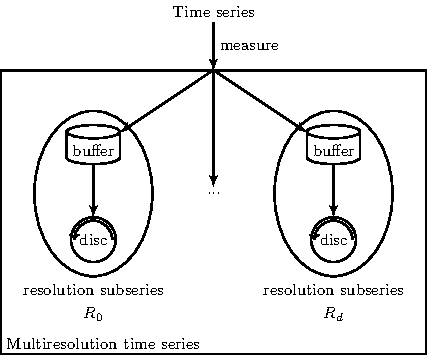
\includegraphics{fig_model_mtsdb.pdf}
  \caption{Architecture of \acro{MTSMS} model}
  \label{fig:model:mtsdb}
\end{figure}

Figure~\ref{fig:model:mtsdb} shows the architecture of a
\acro{MTSMS} for a single multiresolution time series.
%
In this way, the original time series gets stored in the resolution
subseries, each with a different time resolution and distinct
attribute aggregation policies. Discs are size bounded so they only
contain a fixed amount of measures. When a disc becomes full it
discards a measure. Thus, a multiresolution database is bounded in
size and the time series gets stored in a number of storage bounded
time subseries.

Regarding operations, the \acro{MTSMS} model requires two kind of
operators. Some operators should be devoted to set up the time
intervals between measures and to aggregate the attributes. Some other
operators should be dedicated to query the multiresolution schema and
to extract the time series data.

Following, we define the \acro{MTSMS} model structure and the
structural operators, the operations to query a multiresolution
schema, and the \emph{attribute aggregate functions}.  Although schema
manipulation operations could be defined, in this paper we exclusively
focus on structure and data query operators.


\subsection{Structure}

A \emph{buffer} is a container for a time series. The aim of the
buffer is to regularise the time series using a constant
\emph{resolution step} and an \emph{attribute aggregate function}.  We
name \emph{consolidation} to this action of regularisation.  Note that
the attribute aggregate functions are defined in
Section~\ref{sec:model:interpolador}.

\begin{definition}[Buffer]
  Let $S$ be a time series, let $\tau\in\cal{T}$ be the last
  consolidation time, let $\delta\in\cal{T}$ be the resolution step
  and let $f$ be an attribute aggregate function. We define a
  \emph{buffer} $B$ as the tuple $B=(S,\tau,\delta,f)$.
\end{definition}

An empty buffer is noted as $(\emptyset, t_0, \delta, f)$, that is an
empty time series, an initial consolidation time $t_0\in\cal{T}$, a
resolution step $\delta$ and a function $f$.  Given a buffer all the
consolidation time instants can be determined as $\tau_n=t_0+n\delta$
for all $n\in\N$.

Let $B=(S, \tau, \delta, f)$ be a buffer. The \emph{consolidation} of
$B$ is an operation that computes a new measure $m=f(S, \tau, \delta)$
summarising the data of $S$ comprised in the given interval.

A buffer has two main structural operations. The first one adds a
measure to the buffer and the second one consolidates the buffer.

Let $B=(S,\tau,\delta,f)$ be a buffer and let $m$ be a measure.  The
addition of $m$ to $B$, noted as $\addB(B,m)$, returns a new buffer
$\addB(B,m)=(S',\tau,\delta,f)$ where $S' = S \cup \{m\}$.

Let $B=(S,\tau,\delta,f)$ be a buffer. The consolidation of $B$, noted
as $\consB(B)$, returns a new buffer and a new measure $\consB(B)=(B',m')$
where $ B'= (S[\tau+\delta:+\infty], \tau+\delta,\delta,f)$ and $m' =
f(S,\tau,\delta)$. Note that after the consolidation, the
consolidated part of the time series can be removed from the buffer:
historic data is discarded.

The consolidation of a buffer is applied to the first non consolidated
time instant and the total consolidation is obtained by successive
application of the operator. 
%
This requires measures to be added by time order and to consolidate
the buffer when the time of some measure is bigger than the buffer's
next consolidation time.  
%
Let $B=(S,\tau,\delta,f)$ be a buffer and $m=\sup S$ the maximum
measure of $B$. We say that $B$ is consolidable if and only if $T(m)
\geq \tau+\delta$.

A \emph{disc} is a finite capacity container of measures. A time
series stored in a disc has its cardinal bounded. When the cardinal of
the time series is to overcome the limit, some measures need to be
discarded.

\begin{definition}[Disc]
  Let $k\in\N$ and $S$, $|S|\leq k$, be a time series. We define a
  \emph{disc} $D$ as the tuple $D=(S,k)$.
\end{definition}

An empty disc is noted as $(\emptyset,k)$. It is the tuple of an
empty time series and a bound $k$.

The main operation on a disc is to add a measure while keeping under
control the cardinal of the times series. Let $D=(S,k)$ be a disc and
let $m$ be a measure.  The addition of $m$ to $D$, written as
$\addD(D,m)$, is a new disc $\addD(D,m)=(S',k)$ where
%
\[
S' = \begin{cases}
  S\cup\{m\}                 & \text{if } |S|<k  \\
  (S-\{\min S\}) \cup \{m\} & \text{otherwise}
\end{cases}  
\]

A \emph{resolution subseries} is a structure that regularises and
aggregates a time series. It is composed of a buffer, which contains
the time series to be regularised, and a disc, which contains
the regularised time series.


\begin{definition}[Resolution subseries]
  Let $B$ be a buffer and let $D$ be a disc.  We define a
  \emph{resolution subseries} $R$ as the tuple $R=(B,D)$.  
\end{definition}
 
The operators of a resolution subseries extend the buffer and disc
ones. Let $R=(B,D)$ be a resolution subseries and let $m$ be new a
measure.  The addition of $m$ to $R$, noted as $\addR(R,m)$, is a new
resolution subseries $\addR(R,m)=(B',D)$ where $B'= \addB(B,m)$ is the
addition of the measure to the buffer.  The consolidation of $R$,
noted as $\consR(R)$, is a new resolution subseries
$\consR(R)=(B',D')$ where $(B',m') = \consB(B)$ is the consolidation
of the buffer and $D'= \addD(D,m')$ is the addition of the
consolidated measure to the disc. A resolution subseries is
consolidable only when its buffer is consolidable.

A \emph{multiresolution time series} is a set of resolution subseries
referred to the same time series. We store a time series regularised
with distinct resolutions across the resolution subseries, as
previously shown in Figure~\ref{fig:model:mtsdb}.

\begin{definition}[Multiresolution time series]
  Let $M=\{R_0, \dots, R_k\}$ be a finite set of resolution
  subseries. Then $M$ is a \emph{multiresolution time series}.
\end{definition}

Therefore, to define a multiresolution time series we must define the
number of resolution subseries and its corresponding parameters
$(\delta,\tau,f,k)$.  Usually there are no repeated pairs of
$(\delta,f)$ parameters among a multiresolution series, so they act as
key attributes.

The operators of a multiresolution time series apply to every
resolution subseries contained. Let $M=\{R_0,\allowbreak
\dots,\allowbreak R_k\}$ be a multiresolution time series and let $m$
be a measure.
%
The addition of a measure to every resolution subseries, noted as
$\addM(M,m)$, is a new multiresolution time series $\addM(M,m)=\{R'_0,
\dots,\allowbreak R'_k\}$ where $R'_i=\addR(R_i,m)$. The consolidation
of all resolution subseries, noted as $\consM(M)$ is a new
multiresolution time series $\consM(M)=\{R'_0,\allowbreak
\dots,\allowbreak R'_k\}$ where
\[R'_i=
\begin{cases}
\consR(R_i) & \text{if } R_i \text{ consolidable}\\
 R_i & \text{otherwise}
\end{cases}
\]

% The multiresolution consolidation operation should be applied
% regularly based on a consolidation clock. When the measure ordered
% addition approach is taken as explained in the buffer's consolidation,
% then there is no need for a clock in a \acro{MTSMS}. The consolidation
% clock is induced by the measure's addition and then it is only
% necessary to check the multiresolution consolidation operation on new
% additions. However, there could be other approaches where the
% consolidation clock was given by an external clock or external
% events. Then the consolidable definitions would depend on this
% external clock.





\subsection{Queries}

There are two basic time series queries for a \acro{MTSMS}: (i) to
extract a time subseries from a resolution subseries or (ii) to query
for a total time series from all consolidated data.

% Aquesta sembla una consulta una mica circumstancial i menor ...
Let $M$ be a multiresolution time series and let $(\delta,f)$ be a
pair of key attributes.  The first query, denoted as
$\seriedisc(M,\delta,f)$, is a time series such that $\exists (B,D)
\in M: B=(S,\tau,\delta,f) \wedge D=(\seriedisc(M,\delta,f), k) $
where $S,\tau,k$ are bound variables.  Note that we
assume there are no repeated $(\delta,f)$ pairs in $M$.

Let $M=\{R_0,\dots,R_k\}$ be a multiresolution time series and let
$S_0,\dots,S_k$ the time series corresponding to the resolution
subseries $R_0,\dots,R_k$. Assume that the attribute aggregation
functions of all $R_i$ are the same and the resolution steps of all
$R_i$ are distinct.
%
We note as $\totalseries(M)$, the time ordered concatenation of all
time subseries. Recall that $R||S$ is the concatenation for two time
series $R$ and $S$, which has been defined in
Section~\ref{sec:sequence}. Assume that $i_0,\dots,i_k$ is a
permutation of $[0,k]$ such that $\delta_{i_0} < \delta_{i_1} < \cdots
< \delta_{i_k}$ being $\delta_i$ the resolution step of the resolution
subseries $R_i$. Then, $\totalseries(M) = S_{i_0} || S_{i_1} || \cdots
|| S_{i_k}$.
%
TotalSeries obtains the better possible resolution.

From these aforementioned basic time series queries, more elaborated
queries can be applied to \acro{MTSMS} by using \acro{TSMS}
operations. For example, let $L$ and $M$ be two multiresolution time
series, we can compute the sum of both as $\totalseries(L) +
\totalseries(M)$. Recall that $R+S$ is the sum of the values of two
time series $R$ and $S$, which has been defined in
Section~\ref{sec:set} as a binary computational operator.


\subsection{Attribute aggregate function}
\label{sec:model:interpolador}

Attribute aggregate functions are a specific case of \acro{TSMS}
aggregate operations used to summarise time series data while
consolidating a buffer.
%
% Let $S$ be a time series and let $[x,v]$ be a
% time interval. An attribute aggregate function $f$ calculates a new
% measure $m=f(S,[x,v])$. Then, this resulting measure $m$ is interpreted to
% summarise the measures of $S$ for the consolidation interval $[x,v]$.

Let $S$ be a time series, let $\delta$ be a resolution step and let
$\tau$ be a consolidation time.  An \emph{attribute aggregate function} $f$
calculates a new measure $m=f(S,\tau,\delta)$. From $\tau$ and
$\delta$, we obtain the time interval $[\tau:\tau+\delta]$.  Then, the
resulting measure $m$ is interpreted to summarise the measures of $S$
for the time interval $[\tau:\tau+\delta]$.



% \[
% f : S=\{m_0,\ldots,m_k\} \times I=[t_i,t_j] \mapsto m'
% \]
% \[
% f: \cal{P}(\cal{T}\times\cal{V}) \times (\cal{T}\times\cal{T}) \rightarrow \cal{T}\times\cal{V}
% \]

An attribute aggregation function follows this general schema. First,
it obtains a time subseries $S'$ according to the consolidating
interval using a slice operator. For example, $S' =
S[\tau:\tau+\delta]$. Second, it applies a \acro{TSMS} aggregation
function on this time subseries to obtain $m$. For instance, $m =
\agg(S',n, f)$, being $f$ an aggregation function and $n$ an initial
measure, as defined in Section~\ref{sec:set}.

Many different attribute aggregate functions can be used in order to
summarise a time series, for example it is possible to calculate an
statistic indicator of the time series such as the average or a more
complex digital signal processing operation as proposed
by~\cite{zhang11}. Furthermore, the representation of a time series
and some of its pathologies can be considered during the aggregation
process.

Given the diversity of attribute aggregate functions, no global
assumptions can be made about them. Each user should decide which
combination of aggregation and representation fits better to the
measured phenomena.  Therefore, the \acro{MTSMS} model must have a
generic design that allows the users to define their own aggregate
functions.

In what follows we will give some examples of usual attribute
aggregation functions. These functions compute a new measure given a
set of known measures. Then, an attribute aggregation function should
compute a new \emph{time} and a new \emph{value} from the set known measures.
%
% For the rest of this Section we will write $m=f(S,[x,v])$ be the
% resulting measure of an attribute aggregation function $f$ applied to
% a time series $S$ for a time interval $[x,v]$.

% Sobre el calcul del nou temps

The attribute aggregation functions generally return measures that
match the buffer consolidating times. Assume, for instance, that $f$
is an attribute aggregation function and let $m=f(S,\tau,\delta)$.
Then, the time of $m$ is usually computed as $T(m)=\tau+\delta$.
%
However, in some cases it is preferred that $T(m)$ do not match the
buffer consolidating times.
%
For instance, the resulting measure can be aggregated from a time
subseries $S'$ using an open interval $S'=S(\tau:\tau+\delta)$, a
closed interval $S'=S[\tau:\tau+\delta]$, or other combinations like
$S'=S(\tau-d:\tau+\delta-d]$, where $d$ is a time duration that delays the
consolidation to $T(m)=\tau+\delta-d$.
%
This time offset can also be variable. For example, an aggregate
function that returns the first measure of the interval
$m=\min(S[\tau:\tau+\delta))$, then the resulting time fulfils that
$\tau\leq T(m) < \tau+\delta$.

% Sobre el calcul del nou valor
Assume that $f$ is an attribute aggregation function and let
$m=f(S,\tau,\delta)$.  An attribute aggregation function $f$ should
compute the value of $m$.
%
Next there are some examples that illustrate how to compute $V(m)$
based on the temporal function time series operators. 
That is, the time series aggregated is interpreted by the temporal
representation function $S(t)^r$ as has been described in
Section~\ref{sec:model:tfunc}. 
%
In these example functions we leave the time series representation $r$
uninstantiated.

\begin{itemize}
\item The \emph{maximum} computes $V(m)$ as $V(m) =
  \max\limits_{\forall t \in [\tau:\tau+\delta]} S(t)^r$. It
  summarises $S$ with the maximum of the measure values in the
  interval $[\tau:\tau+\delta]$.
\item The \emph{last} computes $V(m)$ as $V(m) = S(\tau+\delta)^r$. It
  summarises $S$ with the value at $\tau+\delta$ time instant.
\item The \emph{mean} computes $V(m)$ as $V(m) = \frac{1}{\delta}
  \int\limits_{\tau}^{\tau+\delta} S(t)^r dt$. It summarises $S$ with
  the mean of the function in the interval $[\tau:\tau+\delta]$.
\end{itemize}

The time series representation in previous examples can be
instantiated in several ways. In what follows we exemplify this
instantiating $r$ as \dd{} and \zohe{}.

Dirac delta attribute aggregation functions interpret the resulting
time as centered on the interval $T(m)=\frac{2\tau+\delta}{2}$. The
resulting value $V(m)$ depends on the attribute, let
$S'=S[\tau:\tau+\delta]^\dd$ be the selection of measures by Dirac
delta temporal interval. Then,
\begin{itemize}
\item The $maximum^\dd$ is such that $V(m) =
  \max\big(0,\max\limits_{\forall n \in S'} V(n)\big)$.
\item The $last^\dd$ is such that $V(m) = V(\max S')$.
\item The $mean^\dd$ is such that $V(m) = \frac{1}{\delta}
  \sum\limits_{\forall n \in S'} V(n)$. Note that for the Dirac
  delta function $\int\dd(t)dt=1$.
\end{itemize}

Note that $\sum\limits_{\forall n \in S'} V(n)$ is a sum of values
that could be implemented as $\agg(S',(0,0),f)$ where
$f(m,n)=(0,V(m)+V(n))$, as shown in
Example~\ref{ex:computational-operators}.

\zohe{} attribute aggregation functions interpret the resulting time
as the right limit of the interval $T(m)=\tau+\delta$. The resulting
value $V(m)$ depends on the attribute, let
$S'=S[\tau:\tau+\delta]^\zohe{}$ be the selection of measures by
\zohe{} temporal interval. Then,

\begin{itemize}
\item The $\maxz$ is such that $V(m) = \max\limits_{\forall n \in S'}
  V(n)$.
\item The $last^\zohe{}$ is such that $V(m) = V(\max S')$.
\item The $\meanz$ is such that $V(m) = \frac{1}{\delta}
  \big[(T(o)-\tau)V(o) + \sum\limits_{\forall n\in R}( T(n)-
  T(\prev_S n) )V(n)\big]$ where $o=\min S'$ and $R= S' - \{o\}$.
\end{itemize}

Note that  $\meanz$ is a sum of values
that could be implemented as $\meanz = \frac{1}{\delta}\agg(S',(0,0),f)$ where $f(m,n)=(0,V(m)+v)$ and 
\[
 v= 
 \begin{cases}
   (T(n)-\tau)V(n) & \text{if } n=\min S'\\
   (T(n)-T(\prev_{S'} n))V(n) & \text{else }
 \end{cases}
\]

\emph{RRDtool}, \cite{rrdtool}, uses an aggregation function similar
to $\meanz$ to summarise velocity counter data by keeping the area
below the original signal.

It is interesting to note that some attribute aggregation patterns are
very similar. For instance, the maximum and last attribute aggregation
schemes differ basically on the interval selection operation. However,
other patterns have a more elaborated interpretation depending on the
actual representation used. This is the case of $\meanz$ and $mean^\dd$.


\begin{example}\label{ex:model:smultiresolution} 
  We define a multiresolution schema for a time series, we consolidate
  the database and we query its data.  Let $S = \{
  (1,6),(5,2),\allowbreak (8,5),\allowbreak (10,0),\allowbreak
  (14,1),\allowbreak (19,6),\allowbreak (22,11),\allowbreak
  (26,6),(29,0) \}$ be a time series and let $M=\{R_0,R_1\}$ be a
  multiresolution time series where each resolution parameters are
  $\tau_0=0$ , $\delta_0=5$, $f_0 =\meanz$, $k_0=4$ and $\tau_1=0$,
  $\delta_1=10$, $f_1 =\maxz$, $k_1=2$. Therefore $R_0$ will be
  consolidated at time instants 5, 10, 15, 20, 25, 30\dots and $R_1$
  at 10, 20, 30\dots

  All measures of $S$ are added to $M$
  and then it is consolidated until it is no more consolidable. As
  $T(\max S)=29$, the last consolidation times are $\tau_0=25$ and
  $\tau_1=20$, so we call $M_{29}$ to the multiresolution time series
  at this state.

  Then, the two time subseries consolidated are obtained by querying
  $\seriedisc(M_{29},5,\allowbreak \meanz)=\{\allowbreak
  (10,3),\allowbreak (15,\allowbreak 2),\allowbreak (20,7),\allowbreak
  (25,8)\}$ and $\seriedisc(M_{29},\allowbreak 10,\allowbreak \maxz)
  =\allowbreak \{ \allowbreak (10,6),\allowbreak (20,11)\}$. Regarding
  buffers, let $S_0$ and $S_1$ be the $M_{29}$ buffer's time series,
  note that $S_0= \{\allowbreak (26,6),\allowbreak (29,0)\allowbreak
  \}$ and $S_1=\{\allowbreak (22,11),\allowbreak (26,6),(29,0)\}$.

  In this particular example,
  $ \totalseries(M_{29}) = \seriedisc(M_{29},\allowbreak 5,\meanz)$ as $R_0$ has
  twice the resolution than $R_1$ and $k_0$ is bigger than $k_1$. 
\end{example}



%%% Local Variables:
%%% TeX-master: "main"
%%% ispell-local-dictionary: "british"
%%% End:

% LocalWords:  genericity multiresolution subseries consolidable

% LocalWords:  pathologies MTSMS TSMS cardinality multivalued infimum
% LocalWords:  multivalues supremum tuple affinely projectively MTSDB
%  LocalWords:  semitemporal piecewise TotalSeries RRDtool


%\part{Experimentació}


\chapter{Introducció a les implementacions}
\label{sec:implementacions}

En aquest capítol implementem \glspl{SGST} i \glspl{SGSTM} segons els
models definits.



Idealment, en un \gls{SGBD} l'usuari executa una consulta i
l'optimitzador s'encarrega d'executar les operacions físiques més
eficients, en aquest sentit el model relacional permet trobar
expressions equivalents donada una determinada consulta. Això no
obstant, i com s'ha detallat en \textref{sec:art:sgbd}, una
implementació de \gls{SGBD} no pot abastar i ser eficient en tots els
àmbits i contextos. Així doncs, no és tan senzill mantenir totalment
la independència entre l'usuari i la implementació ja que cal que
aquest decideixi un \gls{SGBD} adequat per a cada context i fins i tot
que declari com resoldre algunes operacions.  Ara bé, és possible
mantenir la independència del nivell lògic respecte a les
implementacions, i és en aquest sentit que a continuació avaluem
diferents implementacions per als models definits de \gls{SGST} i de
\gls{SGSTM}, on cada implementació està pensada per a un context
determinat.


Anomenem de forma diferent cada implementació que dissenyem per tal de
distingir-les clarament. Són les següents:

\begin{itemize}
\item Pytsms i RoundRobinson: Implementacions a alt nivell per a
  observar el funcionament a nivell acadèmic, amb llenguatge
  Python. Aquesta és la nostra implementació de referència per als
  models de \gls{SGST} i \gls{SGSTM}, la qual a més usem per als
  experiments amb dades.

\item RoundRobindoop: Implementació específica per a la resolució en
  diferit i amb computació para\.lela de la multiresolució, amb model
  de programació MapReduce i en el sistema de computació distribuïda
  Hadoop.

\item Reltsms: Implementació a alt nivell en un \gls{SGBDR}, amb
  llenguatge Tutorial~D i en el sistema Rel.

% \item RoundRobinhard: Implementació a baix nivell d'estructures
%   específiques, amb disseny de circuits digitals o amb llenguatge
%   VHDL. \todo{aquesta va en un apèndix?}


%S'avaluen implementacions específiques com RRDtool?

\end{itemize}

Finalment, en un exemple complet s'experimenta amb les implementacions
amb dades reals. Les implementacions són de programari lliure i els
codis font es poden trobar a \cite{llusa:implementacions}.










\section{Particularitats de les implementacions}



Els models d'implementacions pertanyen al nivell físic dels \gls{SGBD}
i són una realització d'un model lògic, en el nostre cas dels models
lògics de \gls{SGST} i de \gls{SGSTM}. Per a les implementacions se
sol definir el nivell d'usuari, que és el llenguatge que serà visible
per als usuaris. Les implementacions que realitzem volen ser molt
properes al model lògic i per tant el nivell d'usuari que se'n deriva
és molt similar. Per a ser un llenguatge d'usuari complet es
requereixen facilitats i capacitats de llenguatge de programació
--bucles, condicionals, declarar variables, etc.-- per a la qual
cosa ens basem en els recursos particulars de cada implementació:
Python, Tutorial~D, etc. L'objectiu principal, però, d'aquestes
implementacions és acadèmic i per tant no considerem prioritari el
llenguatge d'usuari.

% Aquestes facilitats en el nivell lògic no s'expliciten ja que es
% consideren inherents a les matemàtiques.



En la implementació s'afegeixen alguns operadors que en el model
estructural no havíem definit explícitament perquè ja són propis de
l'àlgebra de conjunts. Així per exemple, alguns d'aquests operadors
que s'han d'implementar són els relacionats amb la notació de creació
de conjunts, %set-builder notation (set comprehension)
els quals en els \gls{SGBD} s'inclouen en el que es coneix com a
\gls{DDL}, o els relacionats amb la manipulació de les dades amb
assignació, inserció, modificació o esborrament, els quals en els
\gls{SGBD} es coneixen com a \gls{DML}.  En el cas dels \gls{SGSTM} sí
que hem definit en el model algunes operacions de \gls{DDL} i \gls{DML} per a
l'esquema multiresolució, ja que aquest requereix ser manipulat
coherentment.

% Pel que fa al llenguatge de consultes (\emph{query language}),
% s'implementa seguint el model d'operacions de consulta de cada cas.





\section{Qüestions de format}

% Llistat: Resultat d’operacions efectuades per un ordinador, escrit en paper per una impressora. en l'àmbit de l'electrònica/informàtica


En els capítols següents s'utilitzen llistats per a mostrar exemples
de funcionament i els resultats de les operacions efectuades.  El
format dels llistats depèn del tipus d'informació que mostren. Així,
bàsicament, els exemples de codi tenen fons gris, com el
\autoref{lst:format:python}, i els exemples de fitxers o sortides per
pantalla tenen fons groc, com el \autoref{lst:format:stdout}.



\begin{lstlisting}[style=py,caption=Exemple de codi,label=lst:format:python]
>>> from pytsms import TimeSeries, Measure as m

>>> s = TimeSeries([m(1,6),m(5,2),m(8,5),m(10,0),m(14,1),m(19,6),m(22,11),m(26,6),m(29,0)])
\end{lstlisting}



\begin{lstlisting}[style=stdout,caption=Exemple de fitxer o de sortida per pantalla,label=lst:format:stdout]
10/maximum_zohe-10	10 0.0
10/maximum_zohe-10	14 1.0
\end{lstlisting}




%%% Local Variables:
%%% TeX-master: "main"
%%% End:


\begin{frame}{Conclusions}

  \begin{itemize}
  \item S'ha situat l'estat actual de l'emmagatzematge i del tractament de sèries temporals.

  \item S'ha estudiat el sistema de gestió de bases de dades RRDtool.

  \item S'ha dissenyat un model que descriu l'estructura i el
    comportament dels SGBD Round Robin per a sèries temporals.
  
  \item S'ha proposat una implementació de referència del model dissenyat.


 \item Un SGBD Round Robin és un sistema informàtic d'emmagatzematge d'una sèrie temporal compactada i repartida segons diferents funcions d'interpolació i períodes de mostreig.

  \end{itemize}

\end{frame}




\begin{frame}{Treball futur}

\begin{itemize}

\item A partir del model RRD es poden estudiar l'aplicació de tècniques d'anàlisis de sèries temporals  i es poden dissenyar SGBD RRD assegurant el funcionament desitjat.


\item Tractament de dades desconegudes. Interpoladors específics.

\item Operacions de consulta: extreure dades, fusionar sèries temporals, visualització, predicció, cerca de patrons, etc.

\item Configurant els interpoladors i els períodes de mostreig s'aconsegueixen reduccions diferents de les sèries temporals.

\item Comprovació amb dades experimentals, (\cite{keogh02}).

\item Variacions en la implementació del model per complir restriccions.

\end{itemize}
\end{frame}


\begin{frame}

\begin{center}
{\huge
Gràcies per l'atenció!
}
\end{center}

\end{frame}

%%% Local Variables: 
%%% mode: latex
%%% TeX-master: "presentacio"
%%% End: 



%------- Annexos ------
%\appendix

%\include{}


%------- Bibliografia ------
\cleardoublepage
%\phantomsection\addcontentsline{toc}{chapter}{\bibname}
\pdfbookmark{\bibname}{bookmark:bibliografia}
\printbibliography



%----------------------------------------------


\end{document}


%%%%%%%%%%%%%%%%%%%%%%%%%%%%%%%%%%%%%%%%%%%%%%%%%%%%%%%%%%%%%%%%%%%%%%%%%%  
% Memòria Tesi de Màster. Estudi i modelització dels SGBD Round Robin pel tractament de sèries temporals.
%
% Copyright (C) 2011-2012 Aleix Llusà Serra.
% 
% This LaTeX document is free software: you can redistribute it and/or
% modify it under the terms of the GNU General Public License as
% published by the Free Software Foundation, either version 3 of the
% License, or (at your option) any later version.
%
% This document is distributed in the hope that it will be useful, but
% WITHOUT ANY WARRANTY; without even the implied warranty of
% MERCHANTABILITY or FITNESS FOR A PARTICULAR PURPOSE. See the GNU
% General Public License for more details.
%
% You should have received a copy of the GNU General Public License
% along with this document. If not, see <http://www.gnu.org/licenses/>.
%
%
% Aleix Llusà Serra
% Departament de Disseny i Programació de Sistemes Electrònics de la Universitat Politècnica de Catalunya (DiPSE-UPC)
% Escola Politècnica Superior d'Enginyeria de Manresa (EPSEM)
% Av. de les Bases de Manresa, 61-73
% 08242 Manresa (Barcelona)
% PAÏSOS CATALANS 
%
% aleix (a) dipse.upc.edu
% 
% El codi font LaTeX del document es troba a 
% <http://escriny.epsem.upc.edu/projects/rrb/>
%%%%%%%%%%%%%%%%%%%%%%%%%%%%%%%%%%%%%%%%%%%%%%%%%%%%%%%%%%%%%%%%%%%%%%%%%%